%#!platex manual; latexml --noparse --destination=./manual.xml manual.tex; latexmlpost --format=xhtml --destination=/tmp/smlsharp/docs/1.0/ja/manual.xhtml --split  --novalidate manual.xml
\documentclass{jbook}

\newif\ifjp
%%%%% 日本語
%  doc/1.0/ja <==== in %#!platex
\jptrue
\newcommand{\txt}[2]{#1}

% %%%%% 英語
% %  doc/1.0/en <==== in %#!platex
% \jpfalse
% \newcommand{\txt}[2]{#2}

\ifjp%>>>>>>>>>>>>>>>>>>>>>>>>>>>>>>>>>>>>>>>>>>>>>>>>>>>>>>>>>>>>>>>>>>>
%% 日本語
\else%%%%%%%%%%%%%%%%%%%%%%%%%%%%%%%%%%%%%%%%%%%%%%%%%%%%%%%%%%%%%%%%%%%%
%% English 
\fi%%%%<<<<<<<<<<<<<<<<<<<<<<<<<<<<<<<<<<<<<<<<<<<<<<<<<<<<<<<<<<<<<<<<<<

\textwidth 15.9truecm
\textheight 24.6truecm
\oddsidemargin 0.0truein
\topmargin -0.5truein

\newcommand{\code}[1]{\mbox{\large\tt #1}}
\newcommand{\module}[2]{\code{#1}(\code{#2})}

\newcommand{\func}{\rightarrow}
\newcommand{\vbar}{\mbox{\ |\ }}
\newcommand{\nonterm}[1]{\mbox{$\langle$}{\it #1}\mbox{$\rangle$}}
\newcommand{\sep}{\mbox{\ \ }}
\newenvironment{program}{\begin{quote}\begin{large}\begin{tt}}%
                        {\end{tt}\end{large}\end{quote}}
\newenvironment{programPlain}{\begin{large}\begin{tt}}%
	                     {\end{tt}\end{large}}
% \newcommand{\myem}{\ \ \ \ \  }
% \newcommand{\myfm}{ \ \ \ \ \ }
\newcommand{\myem}{\ \ }
\newcommand{\myfm}{ \ \ }


\newcommand{\seeJapanese}{The Englishversion is under construction. See
the official Japanese documents.}

\usepackage{latexsym}
\usepackage{url}
\usepackage{epsfig}
\oddsidemargin 0in
\evensidemargin 0in


\renewcommand{\today}{\txt{平成26年3月31日}{March 31, 2014}}
\date{\today}
\newcommand{\smlsharp}{SML\#}

\newcommand{\version}{2.0.0}
\newcommand{\smlsharpSize}{\txt{30万}{0.3 millions}}
% \newcommand{\authors}
% {\txt{大堀\ \ 淳\mbox{\ \ \ \ }上野 雄大}
% {Atsushi Ohori\mbox{\ \ \ \ }Katsuhiro Ueno}
% }
\newcommand{\authors}
{\txt{東北大学 電気通信研究所 \smlsharp{}開発チーム}
{The \smlsharp{} Development Team, RIEC, Tohoku University}
}

\renewcommand{\authors}{}


\title{\txt{プログラミング言語\smlsharp{}解説}{\smlsharp{} Document}}
\author{
\authors
 }

% \includeonly{part5/part5-10}


\begin{document}
% \frontmatter

\maketitle

\part{\txt{概要}{Overview}}
\label{part:outline}

\chapter{\txt{はじめに}{Preface}}

\ifjp%>>>>>>>>>>>>>>>>>>>>>>>>>>>>>>>>>>>>>>>>>>>>>>>>>>>>>>>>>>>>>>>>>>>
	本書は東北大学電気通信研究所で開発された関数型プログラミング言語
\smlsharp{}の公式ドキュメントです.
	\smlsharp{}の概要,プログラミングチュートリアル,参照マニュアル,
ツールなどの情報を含む総合ドキュメントを意図しています.
	関数型言語に慣れた人はもちろん,これからプログラミングを始めようと
する人にも,\smlsharp{}言語を使って高度なプログラミングを書き始めるために
十分な情報を提供します.
	特に,第\ref{part:tutorial}部のチュートリアルは,関数型言語の基
本的な考え方やMLプログラミングの基礎を含んでおり,ML言語の手軽な教科書と
しても使用できます.
	ML言語をより本格的に学ぶには,Standard MLの教科書
\cite{ohori00sml}をご参照ください.
  
	\smlsharp{}は,これら教科書で書かれたStandard MLと後方互換性のあ
る言語です.
	ネイティブコードコンパイラですが,対話型プログラミングもサポート
しており,だれでも手軽にMLプログラミングを楽しむことができます.
	さらに,\smlsharp{}が実現しているC言語とのシームレスな連携などの
機能は,高度で信頼性の要求される本格的な実用的システムの開発にも威力を
発揮すると信じています. 
  
	本ドキュメントを参考に,\smlsharp{}プログラミングをお楽しみくだ
さい. 
	不明な点や要望等は著者にご連絡ください.
\else%%%%%%%%%%%%%%%%%%%%%%%%%%%%%%%%%%%%%%%%%%%%%%%%%%%%%%%%%%%%%%%%%%%%
	This is the official document of \smlsharp{}, a programming
language developed at Research Institute of Electrical Communication,
Tohoku University.
	This document intends to provide comprehensive information on
\smlsharp{}, covering a user's guide, tutorials on ML and \smlsharp{}
programming, and a reference manual.
	This \version{} version only contains an overview of \smlsharp{}
and tutorials on ML and \smlsharp{} programming, which would be
sufficient for beginners who want to start writing ML programs and
for experienced ML programmer who would like to try out or switch to
\smlsharp{}.

	Send comments and questions to the authors.
\fi%%%%<<<<<<<<<<<<<<<<<<<<<<<<<<<<<<<<<<<<<<<<<<<<<<<<<<<<<<<<<<<<<<<<<<

\begin{flushright}
\txt{
2014年3月\\
東北大学電気通信研究所\\
\authors
}
{
March, 2014\\
RIEC, Tohoku University\\
\authors
}
\end{flushright}

\chapter{\txt{本書の使い方}{How to read this document}}

\ifjp%>>>>>>>>>>>>>>>>>>>>>>>>>>>>>>>>>>>>>>>>>>>>>>>>>>>>>>>>>>>>>>>>>>>
    この文書の第\ref{part:outline}部の概要と第\ref{part:tutorial}部のチュー
トリアルはMLプログラミングの基礎から\smlsharp{}が提供する高度の機能まで
を習得できる構造になっています.
	先頭から順に一気にお読みになることをおすすめします.
	お急ぎの方は,以下のページにお探しの情報があるかもしれません.
\begin{itemize}
\item {\bf \smlsharp{}の名前について:}
第\ref{sec:smlsharpHistory}節.
\item {\bf インストール方法:}
第\ref{sec:tutorialInstall}節.
\item {\bf {\tt smlsgarp}コマンドの起動モードと起動パラメタ:}
第\ref{sec:tutorialSmlsharpParameter}節.
\item {\bf \smlsharp{}開発チームと連絡先情報:} 第\ref{sec:smlsharpTeam}節.
\item {\bf \smlsharp{}ホームページ:}
\url{http://www.pllab.riec.tohoku.ac.jp/smlsharp/ja/}
\item {\bf \smlsharp{} Documnet in English:}
\url{http://www.pllab.riec.tohoku.ac.jp/smlsharp/docs/1.0/en/manual.xhtml}
\end{itemize}   

本書に関して,以下の点をご了承ください.
\begin{itemize}
\item 
	現在の第\version{}版のドキュメントはまだ未完成のドラフトです.
	特に,参照マニュアルは含まれず,MLプログラミングのチュートリ
アルも一部未完成です.

\item 随時頻繁に修正を行います.
	そのため,本文書の配布は当面xhtml形式のみとします.
	近い将来,より完成した版のPDFでの配布を検討中です.
\item
	修正・執筆にあたっては,twitterなどでの\smlsharp{}や本書へのコメントな
ども,本書の改善の参考にさせて頂いております.
	個々に言及いたしませんが,本書をご覧頂きコメントをお寄せ頂いた
方々に感謝いたします. 

\item この文書は,LaTeXとLaTeXMLを用いて作成しています.
FirefoxなどのMathMLのレンダリングが可能なブラウザでご覧ください.

\item LaTeXMLは日本語化がなされていないようです.
	本文書は{\tt jbook}クラスで書いていますが,LateXMLのpackageに
jbook用が用意されていないため,{\tt book.cls.ltxml}を
{\tt jbook.cls.ltxml}にコピーし使用しています.
	(LateXMLの日本語クラスパッケージをご存知の方はお教えください.)
\end{itemize}
\else%%%%%%%%%%%%%%%%%%%%%%%%%%%%%%%%%%%%%%%%%%%%%%%%%%%%%%%%%%%%%%%%%%%%

	The tutorials in parts~\ref{part:outline} and
\ref{part:tutorial} are structured in such a way that the reader can
learn from ML programming basics to advanced programming features
provided by \smlsharp{}.
	We recommend to read through these parts quickly in the order
they are presented.

	If you are in a harry, you may find the desired information in
one of the following pages.
\begin{itemize}
\item {\bf How to install \smlsharp{}}: Section \ref{sec:tutorialInstall}.
\item {\bf {\tt smlsharp} command parameters}: Section \ref{sec:tutorialSmlsharpParameter}.
\item {\bf \smlsharp{} development team and contact information}: 
Section \ref{sec:smlsharpTeam}.
\item {\bf On the name of \smlsharp{}}: Section \ref{sec:smlsharpHistory} (History of \smlsharp).
\item {\bf \smlsharp{} web page}: 
\url{http://www.pllab.riec.tohoku.ac.jp/smlsharp/}
\item {\bf \smlsharp{} Documnet in Japanese (プログラミング言語\smlsharp{}解説)}:
\url{http://www.pllab.riec.tohoku.ac.jp/smlsharp/docs/1.0/ja/manual.xhtml}
\end{itemize}

In reading this document, please note the following.
\begin{itemize}
\item 
	This \version{} version is an incomplete draft; it does not
contain the reference manual and the ML programming tutorial is
incomplete.

\item 
	This document is frequently revised and updated.
	For this reason, the currently version is distributed only on
this web server.
	In near future, we plan to include a more complete version of
this document (both in PDF and XHTML format) in the \smlsharp{}
distribution.

\item
	We appreciate those who give us comments on \smlsharp{} and
this document through some communication tools including Twitter.
	We have reflect all of them to the latest version of this
document.

\item 
	This document is written in LaTeX and processed with LaTeXML.
	It is best viewed with a MathML-capable browser such as {\bf Firefox}.
\end{itemize}
\fi%%%%<<<<<<<<<<<<<<<<<<<<<<<<<<<<<<<<<<<<<<<<<<<<<<<<<<<<<<<<<<<<<<<<<<

\chapter{\txt{\smlsharp{}使用上の注意}{Important notes on \smlsharp{}}}

\ifjp%>>>>>>>>>>>>>>>>>>>>>>>>>>>>>>>>>>>>>>>>>>>>>>>>>>>>>>>>>>>>>>>>>>>

\smlsharp{}\version{}版を使用する上で注意すべき点を列挙します.
\begin{enumerate}
\item
%%%%%%%%%%%%%%%%%%ToDo: functorの型引数
\end{enumerate}
\else%%%%%%%%%%%%%%%%%%%%%%%%%%%%%%%%%%%%%%%%%%%%%%%%%%%%%%%%%%%%%%%%%%%%

Here, we list the issues you should aware of in using \smlsharp{}
version~\version{}.
\begin{enumerate}
\item
%%%%%%%%%%%%%%%%%%ToDo: functorの型引数
\end{enumerate}
\fi%%%%<<<<<<<<<<<<<<<<<<<<<<<<<<<<<<<<<<<<<<<<<<<<<<<<<<<<<<<<<<<<<<<<<<

% \tableofcontents
% \mainmatter


\chapter{\txt{\smlsharp{}の概要}{Overview of \smlsharp{}}}
\label{chap:intro}

\ifjp%>>>>>>>>>>>>>>>>>>>>>>>>>>>>>>>>>>>>>>>>>>>>>>>>>>>>>>>>>>>>>>>>>>>
本章では\smlsharp{}言語の概要を説明します.
\else%%%%%%%%%%%%%%%%%%%%%%%%%%%%%%%%%%%%%%%%%%%%%%%%%%%%%%%%%%%%%%%%%%%%
This chapter outlines the \smlsharp{} language and the compiler.
\fi%%%%<<<<<<<<<<<<<<<<<<<<<<<<<<<<<<<<<<<<<<<<<<<<<<<<<<<<<<<<<<<<<<<<<<

\section{\txt{\smlsharp{}とは?}{What is \smlsharp{}?}}
\label{sec:whatIsSmlsharp}

\ifjp%>>>>>>>>>>>>>>>>>>>>>>>>>>>>>>>>>>>>>>>>>>>>>>>>>>>>>>>>>>>>>>>>>>>
\smlsharp{}は,以下のような特徴をもったML系関数型プログラミング言語です.
\begin{enumerate}
\item {\bf Standard MLとの後方互換性.}
	\smlsharp{}は,ML系言語の標準の厳密な仕様であるStandard MLとの
後方互換性を持っています.
	Standard MLの形式的な仕様\cite{sml}を満たすすべての
プログラムをコンパイルできます.

\item {\bf レコード多相性.}
	レコード多相性\cite{ohor95toplas}は,オブジェクトやデータベース
のタプルなどに現れるラベル付きレコードをML言語に完全に統合するために必要
な型システムの機能です.
	\smlsharp{}は,この機能を完全にサポートしています.

\item {\bf SQLのシームレスな統合.}
	SQLはデータベースの標準問い合わせ言語であり,データベースを利用
するプログラムで必ず必要となる機能です.
	\smlsharp{}は,SQLの一部の機能をライブラリとして提供するのでは
なく,SQLクエリそのものを多相型をもつ第一級の式として統合しています.
	この機能により,複雑なプログラムデータベース操作を,MLプログラム
の中で直接プログラムすることができます.
	
\item {\bf C言語との直接連携.}
	システムプログラミングを含む種々のOSの機能の利用にはC言語で記述
されたライブラリへのアクセスが必要となります.
	\smlsharp{}では,名前を外部名宣言するだけで,C言語で書かれCコン
パイラでコンパイルされた関数を呼び出すことができます.

\item {\bf マルチコアCPU上のネイティブスレッドのサポート.}
	\smlsharp{}の並行かつオブジェクトを動かさないGCの機能により,
C言語との連携機能を使い,OSのスレッドライブラリを直接呼び出すことができ
ます.
	従って,OSがマルチコアCPU上での並列実行をサポートしさえすれば,
スレッドを使った高水準なMLプログラムを書き,マルチコアCPU上で効率良く実
効することができます.

\item {\bf 分割コンパイルとリンク.}
	\smlsharp{}は,従来のインクリメンタルなコンパイルではない,真の分
割コンパイルを実現しています.
	各モジュールのインターフェイスの確定後は,各モジュールを独立に開
発しコンパイルやテストできます.
	さらに,\smlsharp{}コンパイラは,分割コンパイルの対象となる各ソー
スコードを,システム標準のオブジェクトファイル(例えばLinuxならば
ELFフォーマット)にコンパイルし,システムのリンカーでCのライブラリなどと
ともにリンクします.
	この機能により,Standard MLだけでなくC言語やSQLなどをも使う
大規模プログラムを安全かつ効率的に開発することができます.

\end{enumerate}

	\smlsharp{}コンパイラおよび実行時処理系は,東北大学電気通信研究
所大堀研究室で開発され,東北大学が著作権保有するオープンソースソフトウェ
アです.
	BSDスタイルの\smlsharp{}ライセンス(\ref{sec:smlsharpLicence}節参照)に
よって公開されており,だれでも自由に利用することができます.
	このライセンスは,二次著作物(つまりコンパイラで作成されたシステ
ムなど)に関する制限の少ないフリーソフトウェアライセンスであり,企業の商
品開発にも安心して使用できます.

\else%%%%%%%%%%%%%%%%%%%%%%%%%%%%%%%%%%%%%%%%%%%%%%%%%%%%%%%%%%%%%%%%%%%%
	\smlsharp{} is a new programming language in the ML-family,
having the following features.
\begin{enumerate}
\item {\bf Downward compatibility with Standard ML.}
	\smlsharp{} can compile all programs that conform to the
definition of the Standard ML\cite{sml}.

\item {\bf Record polymorphism.}
	\smlsharp{} supports record polymorphism \cite{ohor95toplas}.
	In \smlsharp{} , field selection operators {\bf\tt \#\nonterm{label}}
and record patterns {\bf\tt \{\nonterm{field-pat},...\}} are fully
polymorphic.
	This feature is essential in modular development of programs
manipulating records, and is the key to extend ML with SQL.

\item {\bf Seamless integration of SQL.}
	\smlsharp{} seamlessly integrates (currently a subset of) SQL.
	Instead of providing built-in primitives to access
database servers, \smlsharp{} integrate SQL expressions themselves as
polymorphically-typed first-class citizens.
	This allows the programmer to directly access databases in
your polymorphic ML code.

\item {\bf Direct interface to C.}
	\smlsharp{} programs can directly call C functions of your own
coding or in system libraries.
	The programmer need only declare their names and types, without
writing mysterious ``stubs'' or conversion functions. 
	The \smlsharp{} generates external references to C functions,
which are resolved and linked by the system linker.
	Both static and dynamic linking are supported.

\item {\bf Separate compilation and linking.}
	\smlsharp{} supports true separate compilation and linking.
	By writing an interface file, each source file is compiled
separately into an object file in the standard system format (e.g.\ ELF
format.)
	The separately compiled object files are then linked together
possibly with C functions and libraries into an executable program.

\item {\bf Multithread support for multicore CPUs.}
	The non-moving GC \cite{ueno11icfp} and direct C interface allow
\smlsharp{} code to directly call POSIX thread library.
	As far as the OS thread library support a multicore CPU,
\smlsharp{} program automatically obtains multithread capability for
multicore CPUs.
	With the non-moving fully concurrent GC we have just developed, 
concurrent threads run efficiently on a multicore CPU.

\end{enumerate}

	The \smlsharp{} compiler and its runtime system are developed at
Research Institute of Electrical Communication,  Tohoku University.
	They are open-source software distributed with a BSD-style
\smlsharp{} license (\ref{sec:smlsharpLicence}).
\fi%%%%<<<<<<<<<<<<<<<<<<<<<<<<<<<<<<<<<<<<<<<<<<<<<<<<<<<<<<<<<<<<<<<<<<

\section{\txt{\smlsharp{}の歴史}{History of \smlsharp{}}}
\label{sec:smlsharpHistory}

\ifjp%>>>>>>>>>>>>>>>>>>>>>>>>>>>>>>>>>>>>>>>>>>>>>>>>>>>>>>>>>>>>>>>>>>>
	1993年,沖電気工業(株)関西総合研究所にて,大堀により,Standard
ML of New Jerseyコンパイラに多相型レコード演算を加え拡張したプロトタイプ
{\bf SML\# of Kansai}が開発されました.
	その時の\smlsharp{}のtypesメーリングリストへのアナウンスは,今で
もインターネット上に記録されています
(
\url{http://www.funet.fi/pub/languages/ml/sml%23/description}
).

	{\bf SML\# of Kansai}の名前は,このコンパイラにて初めて多相型が与えら
れたレコード演算子"{\bf \code{\#}}"を象徴するものです.
	このコンパイラは,1996年ACM TOPLASに出版されたコード多相性に関する論文
\cite{ohor95toplas}で,{\bf \smlsharp{}}の名前で紹介されています.

	その後,より完全な\smlsharp{}コンパイラの開発の努
力が継続されました.

	2003年に,北陸先端科学技術大学院大学にて,文部科学省リーディング
プロジェクトe-Society基盤ソフトウェアの総合開発「高い生産性をもつ高信頼
ソフトウエア作成技術の開発」
(領域代表者:片山卓也)
の一つの課題
「プログラムの自動解析に基づく高信頼ソフトウェアシステム構築技術」(2003年―2008年,究代表者:大堀 淳)
(
\url{http://www.tkl.iis.u-tokyo.ac.jp/e-society/index.html}
)
として,
次世代ML系関数型言語\smlsharp{}をスクラッチから開発するプロジェクトを開始しました.

2006年4月,プロジェクトは,大堀とともに東北大学電気通信研究所に移り開発
を継続しています.

2008年のe-Societyプロジェクト終了後も,東北大学電気通信研究所大堀研究室
にて,\smlsharp{}の研究開発を続けています.

\else%%%%%%%%%%%%%%%%%%%%%%%%%%%%%%%%%%%%%%%%%%%%%%%%%%%%%%%%%%%%%%%%%%%%

	In 1993, Atsushi Ohori extended the Standard ML of New Jersey
compiler at Kansai Laboratory of Oki Electric, and named the
experimental prototype SML\# of Kansai.
	The Internet still remembers my old posting of \smlsharp{} to
the types mailing list 
(\url{http://www.funet.fi/pub/languages/ml/sml%23/description}).

	The name SML\# of Kansai symbolizes the field selector {\bf\tt
\#\nonterm{label}}, which was given a polymorphic type for the first
time by this compiler.
	This compiler was reported in the ACM TOPLAS article on record
polymorphism \cite{ohor95toplas} as {\bf \smlsharp{}}.

	To support not only record polymorphism but also
interoperability and other practically important features, we decided 
to develop a new SML-style language from scratch, and in 2003, we
started the \smlsharp{} compiler project at Japan Advanced Institute of 
Science and Technology as a part of the e-Society project 
(
\url{http://www.tkl.iis.u-tokyo.ac.jp/e-society/index.html}
).
funded by the Japan ministry of science, education and technologies

	In 2006, the project moved to Tohoku University.
\fi%%%%<<<<<<<<<<<<<<<<<<<<<<<<<<<<<<<<<<<<<<<<<<<<<<<<<<<<<<<<<<<<<<<<<<

\section{
\txt{\smlsharp{}開発チームと連絡先情報}
{\smlsharp{} Development Team and Contact Information}
}
\label{sec:smlsharpTeam}

\ifjp%>>>>>>>>>>>>>>>>>>>>>>>>>>>>>>>>>>>>>>>>>>>>>>>>>>>>>>>>>>>>>>>>>>>
	現在(2014年3月)\smlsharp{}は,
\begin{itemize}
\item 
大堀 淳(東北大学電気通信研究所)
\item 
上野雄大(東北大学電気通信研究所)
\end{itemize}
の2名が,大学院大学院情報科学研究科の大堀研究室に所属の大学院生の協力の
下,開発を行なっています.

	\smlsharp{}のこれまでの主な開発者は以下の通りです.
	(敬称は略させていただいています.
	所属は\smlsharp{}の開発に携わった時のものです.)
\begin{itemize}
\item 大堀 淳(北陸先端科学技術大学院大学情報科学研究科,東北大学電気通信研究所)
\item 大和谷 潔(算譜工房)
\item Nguyen Huu Duc(北陸先端科学技術大学院大学情報科学研究科,東北大学電気通信研究所)
\item Liu Bochao(北陸先端科学技術大学院大学情報科学研究科,東北大学電気通信研究所)
\item 纓坂 智(北陸先端科学技術大学院大学情報科学研究科)
\item 上野雄大(北陸先端科学技術大学院大学情報科学研究科,東北大学電気通信研究所)
\end{itemize}

	東北大学電気通信研究所では,\smlsharp{}に関する情報共有の目的で
以下のwebサイトやメーリングリストを管理しています.
\begin{itemize}
\item \smlsharp{}ホームページ.
\url{http://www.pllab.riec.tohoku.ac.jp/smlsharp/ja/}
コンパイラや本書を含む文書の最新版などもここからダウンロードできます.

\item \smlsharp{}メーリングリスト
{\tt smlsharp@ml.riec.tohoku.ac.jp}.
\smlsharp{}に関する一般的な議論や情報交換のためのメーリングリストです.
使用言語は日本語または英語です.投稿は購読者のみ行うことができ,投稿され
た全てのメールはWeb上に公開されます.\\
%%%%%%%%%%%%%%%%%%ToDo: 参加方法
%参加方法:\url{http://www.pllab.riec.tohoku.ac.jp/mailman/listinfo.cgi/smlsharp-list?language=ja}\\
%アーカイブ:\url{http://www.pllab.riec.tohoku.ac.jp/pipermail/smlsharp-list/}

\item Twitterアカウント {\tt @smlsharp}.
\smlsharp{}に関する最新情報をツイートします.

\item \smlsharp{}開発者への連絡メールアドレス.
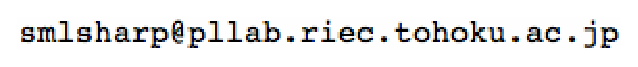
\epsfig{file=smlsharp-list.eps,width=0.4\textwidth}
共同研究の提案や各種問い合わせなどにご利用ください.
\end{itemize}
\else%%%%%%%%%%%%%%%%%%%%%%%%%%%%%%%%%%%%%%%%%%%%%%%%%%%%%%%%%%%%%%%%%%%%
	At present (March 2014), \smlsharp{} is being developed by
\begin{itemize}
\item 
Atsushi Ohori(RIEC, Tohoku University)
\item 
Katsuhiro Ueno (RIEC, Tohoku University)
\end{itemize}
with help of graduate students.

	The past \smlsharp{} development team members include (with the
affiliation at the time of development):
\begin{itemize}
\item Atsushi Ohori (School of Information Science, JAIST; RIEC, Tohoku University)
\item Kiyoshi Yamatodani (Sanpukoubou Inc)
\item Nguyen Huu Duc (School of Information Science, JAIST; RIEC, Tohoku University)
\item Liu Bochao (School of Information Science, JAIST; RIEC, Tohoku University)
\item Satoshi Osaka (School of Information Science, JAIST)
\item Katsuhiro Ueno (School of Information Science, JAIST; RIEC, Tohoku University)
\end{itemize}

	Contact information regarding \smlsharp{}:
\begin{itemize}
\item \smlsharp{} home page:
\url{http://www.pllab.riec.tohoku.ac.jp/smlsharp/ja/}

\item \smlsharp{} mailing list:
{\tt smlsharp-list@pllab.riec.tohoku.ac.jp}

	This list is for general discussion on \smlsharp{}.
	We use Japanese and English in discussion.
	To post a message, you need to subscribe to this list.
	All the messages are made available on the Web.

%%%%%%%%%%%%%%%%%%ToDo: 参加方法
%How to subscribe:\url{http://www.pllab.riec.tohoku.ac.jp/mailman/listinfo.cgi/smlsharp-list?language=ja}\\
%Mail archive:\url{http://www.pllab.riec.tohoku.ac.jp/pipermail/smlsharp-list/}

\item \smlsharp{} twitter account:
{\tt @smlsharp}

	We tweet the latest information about \smlsharp{} on this account.

\item Email address of the \smlsharp{} development team :
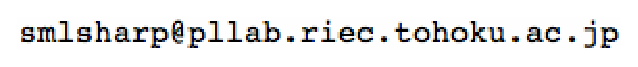
\epsfig{file=smlsharp-list.eps,width=0.4\textwidth}

Send your questions, requests and comments to the development team.
\end{itemize}
\fi%%%%<<<<<<<<<<<<<<<<<<<<<<<<<<<<<<<<<<<<<<<<<<<<<<<<<<<<<<<<<<<<<<<<<<

\section{\txt{謝辞}{Acknowledgments}}
\label{sec:acknowledgements}
	
\ifjp%>>>>>>>>>>>>>>>>>>>>>>>>>>>>>>>>>>>>>>>>>>>>>>>>>>>>>>>>>>>>>>>>>>>
	2003年にスタートした\smlsharp{}開発の過程では,以下を含む色々な
ご指導やご協力を頂きました.
	ここに謝意を表します.
\else%%%%%%%%%%%%%%%%%%%%%%%%%%%%%%%%%%%%%%%%%%%%%%%%%%%%%%%%%%%%%%%%%%%%
	From its start in 2003, we have benefited from many pepples and
ogranizations.
\fi%%%%<<<<<<<<<<<<<<<<<<<<<<<<<<<<<<<<<<<<<<<<<<<<<<<<<<<<<<<<<<<<<<<<<<
	
\subsection{\txt{プロジェクトファンディング}{Project funding}}

\ifjp%>>>>>>>>>>>>>>>>>>>>>>>>>>>>>>>>>>>>>>>>>>>>>>>>>>>>>>>>>>>>>>>>>>>
	\smlsharp{}言語の研究開発は,2003年から5年間の文部科学省リーディ
ングプロジェクトe-Society基盤ソフトウェアの総合開発「高い生産性をもつ高
信頼ソフトウェア作成技術の開発」
(\url{http://www.tkl.iis.u-tokyo.ac.jp/e-society/index.html)}
の一つの課題
「プログラムの自動解析に基づく高信頼ソフトウェアシステム構築技術」(究代
表者:大堀 淳)としてスタートをきることができました.
	このプロジェクトの主要な目標が\smlsharp{}言語コンパイラの開発で
した.
	\smlsharp{}は開発ソースの総量が\smlsharpSize{}行を超える大規模シ
ステムです.
	このプロジェクトの支援がなければ,\smlsharp{}の開発は困難であっ
たと思われます.
	文部科学省,e-Societyの領域代表の片山卓也先生,および関係各位に
深謝いたします.
\else%%%%%%%%%%%%%%%%%%%%%%%%%%%%%%%%%%%%%%%%%%%%%%%%%%%%%%%%%%%%%%%%%%%%
	\smlsharp{} development was started as a part of the 5 year
project 
``e-Society leading project: highly productive reliable software
development technologies (Project Director: Professor Takuya Katayama)'' 
under the title
``
reliable software development technology based on automatic program analysis
(chief investigator: Atsushi Ohori)
''
(\url{http://www.tkl.iis.u-tokyo.ac.jp/e-society/index.html})
sponsored by the Japan ministry of science, education and technologies.
\fi%%%%<<<<<<<<<<<<<<<<<<<<<<<<<<<<<<<<<<<<<<<<<<<<<<<<<<<<<<<<<<<<<<<<<<

\subsection{
\txt{\smlsharp{}が使用しているソフトウエア}
    {Third-party code and software tool used in \smlsharp{} development}
}

\ifjp%>>>>>>>>>>>>>>>>>>>>>>>>>>>>>>>>>>>>>>>>>>>>>>>>>>>>>>>>>>>>>>>>>>>
	\smlsharp{}言語は,第1.0版以降は,\smlsharp{}自身でコンパ
イルし開発を行なっていますが,それ以前は,Standard ML of New Jerseyおよ
びMLtonのStandard MLコンパイラを使って開発を行いました.

	\smlsharp{}は前節(\ref{sec:smlsharpTeam})の開発チー
ムによって開発されたソフトウェアです.
	ソースコードの殆どをスクラッチから開発しましたが,一部に以下のコー
ドを利用しています.

\begin{center}
\begin{tabular}{|l|l|l|}
\hline
内容 & \smlsharp{}ソース上の位置 & ソース
\\\hline
ML-Yacc & src/ml-yacc  & Standard ML of New Jersey 110.73
\\\hline
ML-Lex & src/ml-lex  & Standard ML of New Jersey 110.73
\\\hline
SML/NJ Library & src/smlnj-lib &  Standard ML of New Jersey 110.73
\\\hline
TextIO,
BinIO,
OS,
Timer
&
src/smlnj
&
Standard ML of New Jersey 110.73
\\\hline
浮動小数点/
文字列変換関数
&
src/runtime/netlib
&
the Netlib
\\\hline
SMLFormatの
SML文法定義
&
src/smlformat/generator/main/
&
Standard ML of New Jersey 110.73
\\\hline
\end{tabular}
\end{center}

	これらソースは,いずれも\smlsharp{}ライセンスと整合性あるライセ
ンスで配布されているオープンソースソフトウェアです.
	「\smlsharp{}ソース上の位置」にそれぞれのライセンスが添付されて
います.
\else%%%%%%%%%%%%%%%%%%%%%%%%%%%%%%%%%%%%%%%%%%%%%%%%%%%%%%%%%%%%%%%%%%%%

	Since version 1.0 had completed, \smlsharp{} has been
developed by the \smlsharp{} compiler itself.
	Before the \version{} version, we had used Standard ML of New
Jersey compiler for development and MLTon compiler for building
distributions.

	The \smlsharp{} compiler is a software developed by the
\smlsharp{} development team (\ref{sec:smlsharpTeam}).
	We have wrote most of the code of \smlsharp{} compiler from
scratch, except for the following code: 

\begin{center}
\begin{tabular}{|c|c|c|}
\hline
contents & location in \smlsharp{} distribution & source code
\\\hline
ML-Yacc & src/ml-yacc  & Standard ML of New Jersey 110.73
\\\hline
ML-Lex & src/ml-lex  & Standard ML of New Jersey 110.73
\\\hline
SML/NJ Library & src/smlnj-lib &  Standard ML of New Jersey 110.73
\\\hline
{\tt TextIO},
{\tt BinIO},
{\tt OS},
{\tt Timer}
structures
&
src/smlnj
&
Standard ML of New Jersey 110.73
\\\hline
floating point-string conversion
(dtoa.c)
&
src/runtime/netlib
&
the Netlib
\\\hline
SML grammar definition used 
in SMLFormat tool
&
src/smlformat/generator/main/
&
Standard ML of New Jersey 110.73
\\\hline
\end{tabular}
\end{center}

	All of the above are open-source software that are compatible
with \smlsharp{} license.
	The \smlsharp{} source distribution includes the license of each
of them at the ``location in \smlsharp{} distribution'' show above.
\fi%%%%<<<<<<<<<<<<<<<<<<<<<<<<<<<<<<<<<<<<<<<<<<<<<<<<<<<<<<<<<<<<<<<<<<

\subsection{\txt{研究開発協力者}{Collaborators}}

\ifjp%>>>>>>>>>>>>>>>>>>>>>>>>>>>>>>>>>>>>>>>>>>>>>>>>>>>>>>>>>>>>>>>>>>>
	\smlsharp{}言語の開発にあたっては,多くの人々からの指導を受けま
した.
	過去現在の開発チーム(第(\ref{sec:smlsharpTeam})節)以外で特に
貢献のあった方々は以下の通りです.
\begin{itemize}
\item 篠埜功氏.
大堀と共に,関数フュージョン機能を持つ新たしいインラインの理論および
その実験的な実装を行いました.
	この機能は実験的な実装がありますが,まだ十分な完成度が得られてお
らず\smlsharp{}\version{}版に組み込まれていませんが,将来取り入れたいと
考えています.
\item 大友聡顕氏.
	大堀,上野と共に,オブジェクトを動かさないGCの研究開発に携わり,
初期の実験的な実装を行い,この方式が有望であることを確認しました.
	この成果は,現在のオブジェクトを動かさないGCの方式の開発と実装の
契機となったものです.
\end{itemize}
	これらの方々以外にも,\smlsharp{}は,大堀等との共同で行なった様々
な型理論やコンパイル方式の基礎研究を基に設計されています.
	現在の\smlsharp{}言語に直接生かされている出版された基礎研究成果
には以下のものが含まれます.
\begin{itemize}
\item レコード多相性の理論\cite{ohor92popl,ohor95toplas}.
\item データベースの型推論\cite{ohor88lfp}.
\item データベース言語(Machiavelli)\cite{ohor89sigmod,bune96tods}.
\item ランク1多相性の型理論\cite{ohor99icfp}.
\item MLのunboxed意味論\cite{ohor97unbox}.
\item MLにおける自然なデータ表現\cite{nguyen06ppdp}.
\item オブジェクトを動かさないGC\cite{ueno11icfp}.
\item 軽量の関数融合\cite{ohor07popl}.
\end{itemize}
	それ以外にも多くの共同研究者から色々な機会に示唆や助言を頂いてお
り,それらは1989年にまで遡りますが,それらの方々の列挙は割愛させてい
ただきます.
\else%%%%%%%%%%%%%%%%%%%%%%%%%%%%%%%%%%%%%%%%%%%%%%%%%%%%%%%%%%%%%%%%%%%%

	Many people have contributed to research and development of
\smlsharp{}.
	In addition to the development team (Section
\ref{sec:smlsharpTeam}), the following people directly contributed to 
\smlsharp{} research.
\begin{itemize}
\item Isao Sasano.
With Atsushi Ohori, he investigated 
``Lightweight fusion by fixed point promotion'' and 
developed an experimental inlining module that performs lightweight
fusion.
	This feature is experimental and has not yet been integrated in
\smlsharp{} compiler, but we plan to adopt this method in a future
version.
\item Toshihiko Otomo.
	With Atsushi Ohori and Katsuhiro Ueno, he investigated the
possibility of non-moving collector and showed an initial experimental
result indicating that a non-moving GC is viable in functional
languages.
\end{itemize}
	Many other people helped us through collaborative research with
Atsushi Ohori and others to develop type-theory and compilation methods
that underlie \smlsharp{} compiler.
	\smlsharp{} compiler is directly based on the
following research results, some of them were collaboratively done.
\begin{itemize}
\item record polymorphism \cite{ohor92popl,ohor95toplas}.
\item database type inference \cite{ohor88lfp}.
\item database language (Machiavelli)\cite{ohor89sigmod,bune96tods}.
\item rank-1 polymorphism \cite{ohor99icfp}.
\item unboxed semantics of ML \cite{ohor97unbox}.
\item natural data representation for ML \cite{nguyen06ppdp}.
\item efficient non-moving GC\cite{ueno11icfp}.
\item lightweight fusion \cite{ohor07popl}.
\end{itemize}
	We have also benefited from many other researchers from 1989.
	We refrain from compiling a comprehensive list, which seems to
be impossible. 
\fi%%%%<<<<<<<<<<<<<<<<<<<<<<<<<<<<<<<<<<<<<<<<<<<<<<<<<<<<<<<<<<<<<<<<<<

\section{\txt{\smlsharp{}ライセンス}{\smlsharp{} License}}
\label{sec:smlsharpLicence}

Copyright (c) 2006 - 2014, Tohoku University.\\
All rights reserved.\\

Redistribution and use in source and binary forms, with or without
modification, are permitted provided that the following conditions are
met:

\begin{itemize}
\item 
  Redistributions of source code must retain the above copyright
  notice, this list of conditions and the following disclaimer. 
\item 
  Redistributions in binary form must reproduce the above
  copyright notice, this list of conditions and the following disclaimer
  in the documentation and/or other materials provided with the
  distribution. 
\item 
  Neither the name of Tohoku University nor the names of its
  contributors may be used to endorse or promote products derived from
  this software without specific prior written permission.  
\end{itemize}

THIS SOFTWARE IS PROVIDED BY TOHOKU UNIVERSITY AND CONTRIBUTORS "AS IS"
AND ANY EXPRESS OR IMPLIED WARRANTIES, INCLUDING, BUT NOT LIMITED TO,
THE IMPLIED WARRANTIES OF MERCHANTABILITY AND FITNESS FOR A PARTICULAR
PURPOSE ARE DISCLAIMED. IN NO EVENT SHALL TOHOKU UNIVERSITY OR
CONTRIBUTORS BE LIABLE FOR ANY DIRECT, INDIRECT, INCIDENTAL, SPECIAL,
EXEMPLARY, OR CONSEQUENTIAL DAMAGES (INCLUDING, BUT NOT LIMITED TO,
PROCUREMENT OF SUBSTITUTE GOODS OR SERVICES; LOSS OF USE, DATA, OR
PROFITS; OR BUSINESS INTERRUPTION) HOWEVER CAUSED AND ON ANY THEORY OF
LIABILITY, WHETHER IN CONTRACT, STRICT LIABILITY, OR TORT (INCLUDING
NEGLIGENCE OR OTHERWISE) ARISING IN ANY WAY OUT OF THE USE OF THIS
SOFTWARE, EVEN IF ADVISED OF THE POSSIBILITY OF SUCH DAMAGE.

\section{
\txt{\smlsharp{}第\version{}版の機能と制限}
{Limitations in \smlsharp{} version \version{}}
}
\label{sec:smlsharpLimitation}

\ifjp%>>>>>>>>>>>>>>>>>>>>>>>>>>>>>>>>>>>>>>>>>>>>>>>>>>>>>>>>>>>>>>>>>>>
	我々開発チームは第\ref{sec:whatIsSmlsharp}節でのべた機能をすべて
開発し\smlsharp{}開発開始時に目標とした機能を実現しています.
	第\version{}版にその殆どが含まれていますが,以下の制約があります.
\begin{enumerate}
\item POSIX ネイティブスレッド.
	この機能は現時点では,十分にテストされていないため,デフォルトで
はオフになっています.
	システム構築時({\tt ./configure}時)に{\tt --enable-thread}
を指定すればオンになり,コンパイラはPOSIX thread対応のコードを生成します.
	POSIX thread APIを{\tt \_import}すれば,マルチコア上でネイ
ティブスレッドが利用可能です.

\item ターゲットアーキテクチャ.
	現在の\smlsharp{}コンパイラは,32ビットのIntelアーキテクチャ
(x86, IA-32)向けのコードのみ生成可能です.
	将来,マルチターゲット化を行う予定です.
	特に,Intel系64ビットアーキテクチャ(x64またはamd64)への対応は
近い将来行う予定です.
	\smlsharp{}\version{}版はコンパイラバックエンドにLLVMを用いており,
この対応は容易と思われます.

%\item Windows版の対話型ループの制約.
%	\smlsharp{}\version{}版は,すべて一つのネイティブコードコンパイ
%ラで動いています.
%	対話型ループも,(1)ユーザ入力のコンパイル,
%(2)現在のコンパイラにリンク,
%(3)動的にロード,のサイクルによって実現されています.
%	この中で(2)のリンクをWindowsシステム上で実現するためには,シ
%ステムの制約上,これまでに作られたオブジェクトファイル毎にリンクのための
%ファイルをコマンドラインで指定する必要があります.
%	このファイル数が,対話型環境での入力に従って増えて行きます.
%	そのため,Windows上の対話型環境の連続使用は,コマンドラインの最
%大文字数によって制約されます.

\item 最適化.
	現在のバージョンには,インライニングや定数の伝播などの基本的な最
適化も十分に実装されていません.
	従って,コンパイル時間,コンパイルされたコードの実行時間もともに
十分とは言えません.
%	現在,最適化の設計開発を開始しました.
	将来の版では,他の最適化コンパイラに比肩する速度が得られると期待
しています.
\end{enumerate}
\else%%%%%%%%%%%%%%%%%%%%%%%%%%%%%%%%%%%%%%%%%%%%%%%%%%%%%%%%%%%%%%%%%%%%
	We have successfully developed all the features listed in
Section~\ref{sec:whatIsSmlsharp}, which we had initially aimed at.
	The version \version{} contains most of them, with the following 
restrictions.
\begin{enumerate}
\item {\bf POSIX Native thread support}

	This feature has not yet been well tested.
	So we set it off by default.
	To enable it, give {\tt --enable-thread} to {\tt ./configure}. 
	The compiler then generate thread-safe code.
	If you import OS thread-library through {\tt \_import}
declaration, your multithread code should run on multicore CPU.

	We have also completed development of a fully concurrent
non-moving GC.
	This has not been integrated in \version{} version.
	The GC in the \version{} version is a stop-the-world multithread
extension of the non-moving GC.
	We will replace this with a fully concurrent non-moving GC in
a future version.

\item {\bf Target Architecture.}

	The current compiler only generates x86 (or IA-32) code.
	We plan to support any other platforms, in particular amd64 (or x64),
in near future.
	Since \smlsharp{}\version{} uses LLVM as its compiler backend,
it seems to be easy for \smlsharp{} to support multiple platforms.

\item {\bf Optimization.}

	In this version, optimization is far from adequate; it does not
even implement standard ones such as inlining and constant propagation.
	So both the compilation time and the speed of generated code are
not very satisfactory.
	We have started design and development of optimizing \smlsharp{}
compiler, and hope that we will provide an optimized \smlsharp{}
compiler that is as fast as other mature compilers.

%\item {\bf Interface language.}
%
%	To support separate compilation, we have defined the interface
%language for \smlsharp{} source code.
%	This is our initial design and has a room of improvement.
%	We hope to improve the interface language based on our experience
%and other user's comments and requests.

%\item {\bf SQL integration.}
%
%	The current version only supports PostgreSQL.
%	The available SQL constructs are also limited.
%	In future version, we shall support fuller SQL syntax and
%multiple servers including MySQL.

%\item {\bf Interactive loop on Windows Systems.}
%
%	\smlsharp{} realizes interactive loop by (1) compiling the input
%to an object file, (2) linking with the currently running system to
%generate a dynamically loadable file, and then (3) dynamically loading
%the object code using {\tt dlopen}. 
%	In Windows systems, performing the linking in step 2 requires
%to specify a link information file for each of all the previous object
%files.
%	This implies that the command-line arguments to \smlsharp{}
%compiler uses in step 2 keep increasing during the interactive session,
%and will hit the limit of the command-line length. 
%	At that point, the interactive session may stall.

\end{enumerate}
\fi%%%%<<<<<<<<<<<<<<<<<<<<<<<<<<<<<<<<<<<<<<<<<<<<<<<<<<<<<<<<<<<<<<<<<<

% \section{第1章の用語解説及ぶFAQ}
% \label{sec:glossary1}
% 
% \begin{description}
% \item[BSDスタイルライセンス] 
% 二次著作物に関する制限が少ないオープンソースソフトウェアライセンスの一つ.
% 
% BSDスタイルライセンスでは,ライセンス内容をドキュメント等に表示する限り,
% ソースおよびバイナリ形式をとわず,コードの使用,変更,再配布を認めている.
% これにより,二次著作物,つまりそのソフトを利用して作成される種々の製品を,
% 自由に作成し配布や販売することができる.
% 
% 正確にな内容は英文のBSDライセンス(BSD License,Berkeley Software
% Distribution License)を参照.
% 
% 
% \item[メタ] 
% 「後に」あるいは「越えて」といった位置を表すギリシャ語.
% この接頭語を含むギリシャ語metaphsicaがアリストテレスのよって書かれた名前
% の付けられなかった本の題名の代わに使われることによって,
% 「「自然学」の後に位置する本」という意味のmetaphsicaが,
% その本の内容である「哲学,形而上学(metaphisics)」
% を意味する用語として定着した.
% それに伴い,もともとの位置の概念であったmetaに,自然学を超越する
% という意味が与えられ,種々の分野で使用されようになった.
% たとえば言語学の分野では,metaは,通常の言語の使用を分析するために用いる
% 言語として使用される.
% \end{description}
% 
% FAQ:
% \begin{itemize}
% \item 
% {[Q]} \smlsharp{}の開発に参加したいのですが?\\
% {[A]} もちろん可能です.意欲のある方はご連絡ください.一緒にプログラミング
% 言語の色々な機能を実現していきましょう.今後,研究室以外の人々とのソース
% の共有や変更の管理等の体制を整えていく予定です.
% 
% \item  
% {[Q]} 東北大学電気通信研究所でプログラミングを学ぶことができますか?\\
% {[A]} 東北大学電気通信研究所の不タッフ(教授,准教授,助教)は,学部は工学
% 部,大学院は情報科学研究科または工学研究科大学院の教員を兼務し,工学部知
% 能情報システム総合学科の学部4年生,および教員の所属する情報科学研究科お
% よび工学研究科大学院の学生を受け入れています.大堀研究室は情報科学研究科
% の教員を兼務しています.
% 
% 学部の場合は,工学部知能情報システム総合学科に,大学院なら情報科学研究科
% に入学し大堀研究室を志望すれば,我々と一緒に\smlsharp{}やその他プログラ
% ミング言語及びデータベースの研究開発を思う存分行うことができます.
% 
% \end{itemize}


\include{part2/part2}
\part{\txt{参照マニュアル}{Reference manual}}
\label{part:referenceManual}

\ifjp%>>>>>>>>>>>>>>>>>>>>>>>>>>>>>>>>>>>>>>>>>>>>>>>>>>>>>>>>>>>>>>>>>>>
\else%%%%%%%%%%%%%%%%%%%%%%%%%%%%%%%%%%%%%%%%%%%%%%%%%%%%%%%%%%%%%%%%%%%%
\fi%%%%<<<<<<<<<<<<<<<<<<<<<<<<<<<<<<<<<<<<<<<<<<<<<<<<<<<<<<<<<<<<<<<<<<
	

\part{\txt{プログラミングツール}{Programming Tools}}

\ifjp%>>>>>>>>>>>>>>>>>>>>>>>>>>>>>>>>>>>>>>>>>>>>>>>>>>>>>>>>>>>>>>>>>>>
\else%%%%%%%%%%%%%%%%%%%%%%%%%%%%%%%%%%%%%%%%%%%%%%%%%%%%%%%%%%%%%%%%%%%%
\fi%%%%<<<<<<<<<<<<<<<<<<<<<<<<<<<<<<<<<<<<<<<<<<<<<<<<<<<<<<<<<<<<<<<<<<


\chapter{\txt{構文解析器生成ツール smlyaccとsmllex}{Parser generator smlacc and smllex}}
\ifjp%>>>>>>>>>>>>>>>>>>>>>>>>>>>>>>>>>>>>>>>>>>>>>>>>>>>>>>>>>>>>>>>>>>>
	\smlsharp{}には構文解析器生成ツールsmlyaccが同梱されている.
	このツールはAndrew W. AppelとDavid R. Tarditiによって開発された
ソースコードのプログラムインターフェイスを単純化したものである.
	オリジナルなソフトウェアのライセンス情報は,smlyaccのソースディ
レクトリ\code{src/ml-yacc/COPYRIGHT}に,また,その使い方は
\code{src/ml-yacc/doc/mlyacc.tex}にある.

	ソースファイルの記述方法はオリジナルのものと同一である,
\code{mlyacc.tex}を参照されたい.
\else%%%%%%%%%%%%%%%%%%%%%%%%%%%%%%%%%%%%%%%%%%%%%%%%%%%%%%%%%%%%%%%%%%%%
\fi%%%%<<<<<<<<<<<<<<<<<<<<<<<<<<<<<<<<<<<<<<<<<<<<<<<<<<<<<<<<<<<<<<<<<<

\section{\txt{構文解析システム構造}{Structure of a Parser}}

\ifjp%>>>>>>>>>>>>>>>>>>>>>>>>>>>>>>>>>>>>>>>>>>>>>>>>>>>>>>>>>>>>>>>>>>>
	smlyaccはLRLR構文解析システム構築ツールである.
	ツールの利用には,通常以下のファイルを用意する.
	説明のため,言語
\begin{enumerate}
\item 
\end{enumerate}
	

\else%%%%%%%%%%%%%%%%%%%%%%%%%%%%%%%%%%%%%%%%%%%%%%%%%%%%%%%%%%%%%%%%%%%%
\fi%%%%<<<<<<<<<<<<<<<<<<<<<<<<<<<<<<<<<<<<<<<<<<<<<<<<<<<<<<<<<<<<<<<<<<

\ifjp%>>>>>>>>>>>>>>>>>>>>>>>>>>>>>>>>>>>>>>>>>>>>>>>>>>>>>>>>>>>>>>>>>>>
\else%%%%%%%%%%%%%%%%%%%%%%%%%%%%%%%%%%%%%%%%%%%%%%%%%%%%%%%%%%%%%%%%%%%%
\fi%%%%<<<<<<<<<<<<<<<<<<<<<<<<<<<<<<<<<<<<<<<<<<<<<<<<<<<<<<<<<<<<<<<<<<

\part{\txt{\smlsharp{}の内部構造}{\smlsharp{} Internals and Data Structures}}
\label{part:internals}

\section*{\txt{はじめに}{Preface}}
\ifjp%>>>>>>>>>>>>>>>>>>>>>>>>>>>>>>>>>>>>>>>>>>>>>>>>>>>>>>>>>>>>>>>>>>>
	第\ref{part:internals}部では,\smlsharp{}コンパイラの内部構造を
詳述する.
	本部の目的は,本文書の第\ref{part:tutorial}部などを習得しML系関
数型言語の素養を持つ者が\smlsharp{}ソースコードの詳細を理解することである.
	読者としては,\smlsharp{}コンパイラの開発に加わろうとする者や
\smlsharp{}ソースコードを新しいコンパイラ開発等に利用しようとする者を主
に想定しているが,高水準プログラミング言語のコンパイラに興味を持つ一般の
読者にも参考となる文書となるように配慮した.

	オープンソースソフトウェアには尊敬すべき優れたコードが数多く存在
するが,それらの文化に接して筆者が感じる問題点の一つは,それら優れたコー
ドの構造や機能を,他の開発者や興味ある読者に理解できるように文書化する努
力が往々にして欠如していることである.
	コードそれ自体がドキュメントであるとの主張は,極端に規模の小さい
コードには当てはまるものの,数万行を超える大規模システムに対しては現実的
ではない.
	大規模システムでは,コード断片にはそのコード自身では理解不可能な
大域的な仮定や,他の複数のコード断片を制御するためのデータが含まれる.
	それらを理解するには,関連するシステム全般に関する処理の流れと,
その実現のためにシステムの各部分に分散してコード化されたデータの意味の全
体象を把握する必要がある.
	この大規模システムの複雑化に対処する現時点での唯一の方法は文書化
であると考える.
	さらに,コードの意図や構造を記述した文書は,それ自身,新たな構造
や機能の示唆を与えうる財産となると期待される.

	そこで,本文書では,その範を,筆者が尊敬するVAX/VMS OSの内部構造
の詳細な記述文書\cite{Kenah:1984:VID:225}に取り,\smlsharp{}コードが扱う
データ構造とコードの処理の詳細を,各機能が基礎とする理論やアルゴルズムと
共に記述することにした.
	本書が,\smlsharp{}のソースコードの開発や改良に取り組もうとする
者の理解の助けとなり,\smlsharp{}開発コミュニティ形成に資することを願う.

	第\ref{part:internals}部の構成は以下の通りである.
\begin{enumerate}
\item 第\ref{chap:package}章で\smlsharp{}ソースパッケージの構成を記述する.
\item 
      第\ref{chap:SimpleMain}章から第\ref{chap:LLVMCodegeneration}章までは,
\smlsharp{}コンパイラが操作するデータ構造とソースコードの詳細を,各フェー
ズ毎に記述する.
	コンパイルフェーズは通常複数のストラクチャから構成され,それら関
連するストラクチャは一つのディレクトリに置かれている.
	これら各章では,概ねディレクトリ単位でひとまとまりの処理を記述す
る. 
	補助的に使われているモジュールの機能を簡潔に記述した後,主要な処
理を行うモジュールの詳細を記述する.
\item 第\ref{chap:sqlintegration}章から第\ref{chap:interactivemode}章ま
での章では,フェーズにまたがる処理を記述する.
\item 第\ref{chap:bootstraping}章では,\smlsharp{}を拡張するためのブートスト
ラップ手順を記述する.
\item 第\ref{chap:runtimesystem}章では,\smlsharp{}の実行時処理系を記述
する.
\item 第\ref{chap:buildsystem}章では,\code{Makefile}の構成を含む,
\smlsharp{}コンパイラをコンパイルリンクするための環境を解説する.
\end{enumerate}
\else%%%%%%%%%%%%%%%%%%%%%%%%%%%%%%%%%%%%%%%%%%%%%%%%%%%%%%%%%%%%%%%%%%%%
	This part presents internals and data structures of the
\smlsharp{} compiler.
	The primiary readers are the developpers of the \smlsharp{}
compiler and all those who use the \smlsharp{} source code to extend and
modify the compiler. 
	To serve as a reference document on a full-scale compiler, which
can be read independenly, we also include the rationale, algorithms,
theories that underlie the compiler design and implementation. 

	Part \ref{part:internals} contains the following.
\begin{enumerate}
\item Chapter \ref{chap:package} describes the \smlsharp{} distribution
package.
\item 
      The chapters from Ch.\ref{chap:SimpleMain} to
Ch.\ref{chap:LLVMCodegeneration} describes the data structures and the
source code of each compilation phase in the order the compiler
processes  the source file.
\item 
	The chapters from Ch.\ref{chap:sqlintegration} to
Ch.\ref{chap:interactivemode} describes the processes that span
multiple compilation phases.
\item Chapter \ref{chap:bootstraping} describes the standard steps to
bootstrap the \smlsharp{} compiler.
\item 
	Chapter \ref{chap:runtimesystem} describes the runtime system.
\item 
	Chapter \ref{chap:buildsystem} describes data files such as
\code{Makefile} and various supporting scripts used to build the
\smlsharp{} system. 
\end{enumerate}
\fi%%%%<<<<<<<<<<<<<<<<<<<<<<<<<<<<<<<<<<<<<<<<<<<<<<<<<<<<<<<<<<<<<<<<<<


\chapter{\txt{\smlsharp{}パッケージの構造}{The Structure of \smlsharp{} Distribution}}
\label{chap:package}

\ifjp%>>>>>>>>>>>>>>>>>>>>>>>>>>>>>>>>>>>>>>>>>>>>>>>>>>>>>>>>>>>>>>>>>>>
	\smlsharp{}配布パッケージ\code{smlsharp-2.0.0.tar.gz}は,
\smlsharp{}コンパイラ,基本ライブラリ,サポートツールのソースを含む.
	本章では,\code{smlsharp-2.0.0.tar.gz}の構造を記述する.
\else%%%%%%%%%%%%%%%%%%%%%%%%%%%%%%%%%%%%%%%%%%%%%%%%%%%%%%%%%%%%%%%%%%%%
	\smlsharp{} distribution packabe \code{smlsharp-2.0.0.tar.gz}
contains the sources and other resources for the \smlsharp{} compiler,
the Standard ML Basis library, and several supporting tools.
	This chapter describes the major components of
\code{smlsharp-2.0.0.tar.gz}.
\fi%%%%<<<<<<<<<<<<<<<<<<<<<<<<<<<<<<<<<<<<<<<<<<<<<<<<<<<<<<<<<<<<<<<<<<

\section{\txt
{\smlsharp{}ソースパッケージの構成}
{The Source Distribution of the \smlsharp{} Compiler}
}

\ifjp%>>>>>>>>>>>>>>>>>>>>>>>>>>>>>>>>>>>>>>>>>>>>>>>>>>>>>>>>>>>>>>>>>>>
	\smlsharp{}のソースディストリビューション
\code{smlsharp-2.0.0.tar.gz}には以下のファイルが含まれる.

\begin{tabular}{ll}
\code{src/} &  ソースファイルディレクトリ\\
\code{sample/}& サンプルプログラムディレクトリ\\
\code{benchmark/}& Standard MLベンチマークソース.\\
\code{test/}& テストのためのリソースディレクトリ.(将来整備予定.)\\
\code{precompiled/}& \code{minismlsharp}のアセンブリソースファイル\\
\code{configure.ac}& \code{autoconf}への入力ファイル\\
\code{Makefile.in}& \code{Makefile}ファイルテンプレート\\
\code{config.h.in}& \code{config.h}ファイルテンプレート\\
\code{config.mk.in}& \code{Makefile}の動作を制御する\code{config.mk}ファイルテンプレート\\
\code{depend.mk}& \code{Makefile}で参照されるファイルの依存関係を記述したファイル.\\
\code{files.mk}& \code{Makefile}で参照される種々のファイル集合定数の定義ファイル.\\
\code{mkdepend}& \code{depend.mk}を作成に使用するスクリプト.\\
\code{precompile.mk}& \code{precompiled/}再構築用\code{make}ファイルスクリプト.\\
\code{RELEASE\_DATE} & リリース版日付\\
\code{VERSION} & バージョン\\
\code{Changes} & リリース情報ファイル\\
\code{INSTALL} & インストール手順の記述\\
\code{LICENSE} & \smlsharp{}ライセンス
\end{tabular}
\else%%%%%%%%%%%%%%%%%%%%%%%%%%%%%%%%%%%%%%%%%%%%%%%%%%%%%%%%%%%%%%%%%%%%
	\smlsharp{} source sidtribution package 
\code{smlsharp-2.0.0.tar.gz} contains the following files and
directories.

\begin{tabular}{ll}
\code{src/} & the source directory
\\
\code{sample/} & sample programs
\\
\code{benchmark/} & Standard ML benchmark programs.
\\
\code{test/} & a unit test framework. (Currently not functional; it will
be activated in future.)
\\
\code{precompiled/} & assembry file archives to build
\code{minismlsharp} for compiling \smlsharp{} source codes.
\\
\code{configure.ac} & input to \code{autoconf}
\\
\code{Makefile.in} & \code{Makefile} tamplate.
\\
\code{config.h.in} & \code{config.h} tamplate.
\\
\code{config.mk.in} &
	\code{config.mk} template containing configuration parameters used in \code{Makefile}.
\\
\code{files.mk} & Auto-generated file that defines variables used in
\code{Makefile}.
\\
\code{mkdepend} & The shell script for generating \code{depend.mk}
\\
\code{precompile.mk} & a \code{make} script for generating
    \code{precompiled/} acrchives.
\\
\code{RELEASE\_DATE} & the release date
\\
\code{VERSION} &  the current version
\\
\code{Changes} &  the change history
\\
\code{INSTALL} & install instructions
\\
\code{LICENSE} & \smlsharp{} license
\end{tabular}
\fi%%%%<<<<<<<<<<<<<<<<<<<<<<<<<<<<<<<<<<<<<<<<<<<<<<<<<<<<<<<<<<<<<<<<<<

\section{\txt
{\smlsharp{} ソースツリー}
{The \smlsharp{} Source Tree}
}

\ifjp%>>>>>>>>>>>>>>>>>>>>>>>>>>>>>>>>>>>>>>>>>>>>>>>>>>>>>>>>>>>>>>>>>>>
	\smlsharp{}コンパイラのソースは,\code{src}ディレクトリ下の以下
の各ディレクトリに分割して格納されている.

\begin{tabular}{ll}
\code{compiler/} & \smlsharp{}コンパイラ
\\
\code{basis/} & Standard ML基本ライブラリ
\\
\code{compiler-utils/} & \smlsharp{}コンパイラが使用する汎用ライブラリ
\\
\code{config/} & \code{configure}が設定するシステムパラメタアクセスライブラリ.
\\
\code{ffi/} & \smlsharp{}のC言語インターフェイスサポートライブラリ.
\\
\code{reifiedterm/} & コンパイラ環境にアクセスするための自己反映ライブラリ.
\\
\code{sql/} & \smlsharp{}のSQL統合機能を使用するためのサポートライブラリ.
\\
\code{unix-utils/}& Unixの基本コマンドライブラリ.
\\
\code{runtime/} & \smlsharp{}実行時環境.
\\
\code{llvm/} & LLVMコード生成ライブラリ.
\\
\code{smlnj/} & \smlsharp{}が使用している\code{smlnj}のStandard ML基本ライブラリソースファイル.
\\
\code{smlnj-lib/} & \code{smlnj}のユーティリティライブラリ.
\\
\code{smlformat/} & プリンター自動生成ツール\code{smlsormat}.
\\
\code{ml-lex/} & \code{smllex}ソースファイル.
\\
\code{ml-yacc/} & \code{smlyacc}ソースファイル.
\\
\code{basis.smi} & 基本ライブラリのインターフェイルファイル.
\\
\code{builtin.smi} & コンパイラの組込環境の設定ファイル.
\\
\code{prelude.smi} & \smlsharp{}の対話型環境のインターフェイスファイル.
\\
\code{ffi.smi} & C連携機能の利用のためのインターフェイルファイル.
\\
\code{sql.smi} & SQL統合機能の利用のためのインターフェイルファイル.
\\
\code{smlformat-lib.smi} & \code{smlformat}のライブラリインターフェイスファイル.
\\
\code{ml-yacc-lib.smi} & \code{smlyacc}のライブラリインターフェイスファイル.
\\
\code{config.mk.in} & コンパイラの\code{make}環境設定用テンプレートファイル.
\end{tabular}

\else%%%%%%%%%%%%%%%%%%%%%%%%%%%%%%%%%%%%%%%%%%%%%%%%%%%%%%%%%%%%%%%%%%%%
	\code{src} directory contains the sources for the following.

\begin{tabular}{ll}
\code{compiler/}& the \smlsharp{} compiler
\\
\code{basis/}&  the Standard ML Basis Library
\\
\code{compiler-utils/}&  basic libraries ussed in the \smlsharp{} compiler
\\
\code{config/}& the to access \code{configure} parameters
\\
\code{ffi/}&  a support library for \smlsharp{} C interface
\\
\code{reifiedterm/}& a reflection library to access access \smlsharp{}
    compiler environments.
\\
\code{sql/}& a support library for \smlsharp{} SQL integration
\\
\code{unix-utils/}& basic Unix command libraries
\\
\code{runtime/}&  the \smlsharp{} runtime system
\\
\code{smlformat/}&  the pretty printer generator
\\
\code{smlnj/}&  SMLNJ sources for Standard ML Basis Library used by the \smlsharp{}
\\
\code{smlnj-lib/}&  \code{smlnj} utility libraries
\\
\code{ml-lex/}& \code{smllex} addapted from Tarditi and Appel implementation
\\
\code{ml-yacc/}& \code{smlyacc} addapted from Tarditi and Appel implementation
\\
\code{basis.smi}&  the interface file to bind the Standard ML Basis Library
\\
\code{builtin.smi}& the interface file used in \smlsharp{} to set up its
    builtin environment
\\
\code{ffi.smi}&  the interface file to enable C language FFI
\\
\code{ml-yacc-lib.smi}&  the interface file to load \code{smlyacc} resources
\\
\code{prelude.smi}&  the interface file to set up the initial interactive environment
\\
\code{smlformat-lib.smi}& the interface file to load \code{smlformat} resources
\\
\code{sql.smi}& the interface file to enable SQL integration
\\
\code{config.mk.in}&  a template file to set up \code{make} parameters
\\
\end{tabular}
\fi%%%%<<<<<<<<<<<<<<<<<<<<<<<<<<<<<<<<<<<<<<<<<<<<<<<<<<<<<<<<<<<<<<<<<<

\section{\txt{\code{compiler}ディレクトリ}{The \code{compiler} Directory}}
\ifjp%>>>>>>>>>>>>>>>>>>>>>>>>>>>>>>>>>>>>>>>>>>>>>>>>>>>>>>>>>>>>>>>>>>>
	\smlsharp{}コンパイラ本体のソースファイルのディレクトリである.
	このディレクトリは,以下に示すコンパイラのフェーズや中間言語等の
主要なデータ構造毎にサブディレクトリに分割されている.
\begin{enumerate}
\item 
	コンパイラの中間言語

\begin{tabular}{ll}
\code{absyn/}& 抽象構文木
\\
\code{constantterm/}& コンスタント定義
\\
\code{patterncalc/}& 型無し中間表現
\\
\code{types/}& 型定義,IDを変数名とする型無し中間言語
\\
\code{typedcalc/}& 型付き中間言語
\\
\code{recordcalc/}& 型付きレコード計算
\\
\code{typedlambda/}& 型付きラムダ計算
\\
\code{bitmapcalc/}& ビットマップを明示した中間言語
\\
\code{closurecalc/}& クロージャ中間言語
\\
\code{runtimetypes/}& 実行時型表現
\\
\code{runtimecalc/}& 低レベル中間言語
\\
\code{anormal/}& A-normal中間言語
\\
\code{machinecode/}& 低レベルコード言語
\\
\code{llvmir/}& LLVMコード
\end{tabular}

\item コンパイルフェーズ 

\begin{tabular}{ll}
\code{main/}& メインモジュール
\\
\code{toplevel2/}& コンパイラトップレベル
\\
\code{parser2/}& 構文解析
\\
\code{loadfile/}& インターフェイスローディング処理
\\
\code{generatemain/}& メイン関数名生成処理
\\
\code{elaborate/}& 構文論的評価
\\
\code{nameevaluation/}& 名前評価とモジュールコンパイル
\\
\code{valrecoptimization/}& 相互再帰的関数最適化処理
\\
\code{reflection/}& コンパイラ環境の自己反映処理,プリンタ生成処理
\\
\code{typeinference2/}& 型推論,カリー関数最適化
\\
\code{typedcalcoptimization/}& 型付き中間言語最適化
\\
\code{matchcompilation/}& パターンマッチングコンパイル
\\
\code{sqlcompilation/}& 型依存SQLコンパイル
\\
\code{fficompilation/}&  C言語連携コンパイル
\\
\code{recordcompilation/}& 型主導レコードコンパイル
\\
\code{recordcalcoptimization/}& 型付きレコード計算最適化処理
\\
\code{datatypecompilation/}& データ型コンパイル
\\
\code{bitmapcompilation2/}& ビットマップ生成
\\
\code{closureconversion/}& クロージャ変換
\\
\code{cconvcompile/}& コーリングコンベンションコンパイル
\\
\code{anormalize/}& A-normal変換
\\
\code{machinecodegen/}&  低レベルコード生成
\\
\code{stackallocation/}& スタックフレーム割り当て
\\
\code{llvmgen/}& LLVMコード生成
\\
\code{llvmemit/}& LLVMコードエミッション
\end{tabular}

\item コンパイル環境設定,ユーテリティ

\begin{tabular}{ll}
\code{builtin2/}& コンパイラ組込環境
\\
\code{control/}& コンパイラ制御パラメタ
\\
\code{name/}& シンボル及びIDの定義
\\
\code{util/}& ユーティリティライブラリ
\\
\code{toolchain/}& Unixのtoolchainバインディング
\\
\code{usererror/}& エラー登録処理
\end{tabular}

\item 将来再インストールする予定のモジュール

\begin{tabular}{ll}
\code{functionlocalize/}& 関数局所化最適化
\\
\code{recordunboxing/}& レコードUnbox最適化
\\
\code{staticanalysis/}& 静的コード解析
\end{tabular}
\end{enumerate}
\else%%%%%%%%%%%%%%%%%%%%%%%%%%%%%%%%%%%%%%%%%%%%%%%%%%%%%%%%%%%%%%%%%%%%

	This is the source directory of the \smlsharp{} compiler
function containg the following.

\begin{enumerate}
\item 
	Compiler intermediate languages.

\begin{tabular}{ll}
\code{absyn/}& the abstract syntax tree
\\
\code{constantterm/}& constant definitions
\\
\code{patterncalc/}& the untyped intermediate language
\\
\code{types/}& type definitions, the id-based scope-free untyped intermediate language
\\
\code{typedcalc/}& the typed intermediate language
\\
\code{recordcalc/}& the typed record calculus
\\
\code{typedlambda/}& the typed lambda calculus
\\
\code{bitmapcalc/}& the typed intermediate language with explicit layout bitmap
\\
\code{closurecalc/}& the typed intermediate language with explicit closures
\\
\code{runtimetypes/}& runtime type definitions
\\
\code{runtimecalc/}& the typed intermediate language with runtime types
\\
\code{anormal/}& the A-normal forms
\\
\code{machinecode/}& the low-level intermediate language
\\
\code{llvmir/}& the LLVM code
\end{tabular}

\item Compilation phases

\begin{tabular}{ll}
\code{main/}& main function
\\
\code{toplevel2/}& compiler top-level
\\
\code{parser2/}& parser
\\
\code{loadfile/}& interface loading
\\
\code{generatemain/}& main function name generation
\\
\code{elaborate/}& syntactic elaboration
\\
\code{nameevaluation/}& name evaluation and module compilation
\\
\code{valrecoptimization/}& mutual recursive function optimization
\\
\code{reflection/}& compile-time reflection and printer code generation
\\
\code{typeinference2/}& type definition,uncurry optimization
\\
\code{typedcalcoptimization/}& typed intermediate language optimization
\\
\code{matchcompilation/}& pattern matching compilation
\\
\code{sqlcompilation/}& type-directed SQL server-declaration compilation
\\
\code{fficompilation/}& C interface generation for higher-order functions
\\
\code{recordcompilation/}& type-directed record compilation
\\
\code{recordcalcoptimization/}& typed record calculus optimization
\\
\code{datatypecompilation/}& datalayout computation
\\
\code{bitmapcompilation2/}& explicit layout-bitmap generation
\\
\code{closureconversion/}& closure conversion
\\
\code{cconvcompile/}& type-directed calling-convention generation
\\
\code{anormalize/}& a-normalization
\\
\code{machinecodegen/}&  law-level code generation
\\
\code{stackallocation/}& stack frame allocation
\\
\code{llvmgen/}& llvm code generation
\\
\code{llvmemit/}& llvm code emmition
\end{tabular}

\item Compiling environments and utilities

\begin{tabular}{ll}
\code{builtin2/}& the compiler built-in environment
\\
\code{control/}& compilation parameters
\\
\code{name/}& symbol and idntifier definitoions
\\
\code{util/}& compiler utilities
\\
\code{toolchain/}& Unix toolchain bindings
\\
\code{usererror/}& error handling
\end{tabular}

\item modules to be installed in future

\begin{tabular}{ll}
\code{functionlocalize/}& function localization optimization
\\
\code{recordunboxing/}& record unboxing optimization
\\
\code{staticanalysis/}& static intermediate language analysis for optimization
\end{tabular}
\end{enumerate}
\fi%%%%<<<<<<<<<<<<<<<<<<<<<<<<<<<<<<<<<<<<<<<<<<<<<<<<<<<<<<<<<<<<<<<<<<

\ifjp%>>>>>>>>>>>>>>>>>>>>>>>>>>>>>>>>>>>>>>>>>>>>>>>>>>>>>>>>>>>>>>>>>>>
	\code{src}下の各サブディレクトリは,\code{main}サブディレクトリ
を含み,このディレクトリ以下にソースファイルが置かれている.
	従って,例えば抽象構文木のソースファイルは\code{absyn/main/}下に
置かれている.
	この構成は,各コンパイラの構成要素の検証やテストのためのリソース
を配置することを意図したものである.
	現時点では,各サブディレクトリは\code{main}以外のディレクトリを
持たない.

	\code{xxx/main/}以下には,通常,拡張子\code{.sml}を持つソースファ
イルと拡張子\code{.smi}を持つ同名のインターフェイスファイルを含む.
	以下の拡張子を持つファイルは,ソースファイルを生成するための入力
ファイルである.

\begin{tabular}{ll}
\code{.ppg} &
\code{smlformat}の入力ファイル.
プリンターコードが自動生成される.
通常,データ型定義ファイルである.
\\
\code{.grm} &
\code{smlyacc}の入力ファイル.
\\
\code{.lex} &
\code{smllex}の入力ファイル.
\end{tabular}

	\code{make}システムで\smlsharp{}をビルドする過程で,これらのファ
イル対するソースファイルが生成される.
	ディレクトリに用意されている\code{.smi}が付加したインターフェイ
スファイルは,自動生成されたソースファイルのインタフェイス記述である.
\else%%%%%%%%%%%%%%%%%%%%%%%%%%%%%%%%%%%%%%%%%%%%%%%%%%%%%%%%%%%%%%%%%%%%
	\code{src}下の各サブディレクトリは,\code{main}サブディレクトリ
を含み,このディレクトリ以下にソースファイルが置かれている.
	従って,例えば抽象構文木のソースファイルは\code{absyn/main/}下に
置かれている.
	この構成は,各コンパイラの構成要素の検証やテストのためのリソース
を配置することを意図したものである.
	現時点では,各サブディレクトリは\code{main}以外のディレクトリを
持たない.

	\code{xxx/main/}以下には,通常,拡張子\code{.sml}を持つソースファ
イルと拡張子\code{.smi}を持つ同名のインターフェイスファイルを含む.
	以下の拡張子を持つファイルは,ソースファイルを生成するための入力
ファイルである.
\begin{itemize}
\item \code{.ppg} \code{smlformat}の入力ファイル.
	プリンターコードが自動生成される.
	通常,データ型定義ファイルである.
\item \code{.grm} \code{smlyacc}の入力ファイル.
\item \code{.lex} \code{smllex}の入力ファイル.
\end{itemize}
	\code{make}システムで\smlsharp{}をビルドする仮定で,これらのファ
イル対するソースファイルが生成される.
	ディレクトリに用意されている\code{.smi}が付加したインターフェイ
スファイルは,自動生成されたソースファイルのインタフェイス記述である.
\fi%%%%<<<<<<<<<<<<<<<<<<<<<<<<<<<<<<<<<<<<<<<<<<<<<<<<<<<<<<<<<<<<<<<<<<

\section{\txt{\code{basis}ディレクトリ}{The \code{basis} Directory}}
\ifjp%>>>>>>>>>>>>>>>>>>>>>>>>>>>>>>>>>>>>>>>>>>>>>>>>>>>>>>>>>>>>>>>>>>>
	基本ライブラリのソースファイルである.
	\code{main}ディレクトリ以下に以下のファイルを含む.

\begin{enumerate}
\item シグネチャファイル.
	拡張子\code{.sig}を持つ以下のファイル.
	ファイル名がシグネチャ名に対応している.

\begin{tabular}{l}
\code{ARRAY.sig}\\
\code{ARRAY\_SLICE.sig}\\
\code{BIN\_IO.sig}\\
\code{BOOL.sig}\\
\code{BYTE.sig}\\
\code{CHAR.sig}\\
\code{COMMAND\_LINE.sig}\\
\code{DATE.sig}\\
\code{GENERAL.sig}\\
\code{IEEE\_REAL.sig}\\
\code{IMPERATIVE\_IO.sig}\\
\code{INTEGER.sig}\\
\code{INT\_INF.sig}\\
\code{IO.sig}\\
\code{LIST.sig}\\
\code{LIST\_PAIR.sig}\\
\code{MATH.sig}\\
\code{MONO\_ARRAY.sig}\\
\code{MONO\_ARRAY\_SLICE.sig}\\
\code{MONO\_VECTOR.sig}\\
\code{MONO\_VECTOR\_SLICE.sig}\\
\code{OPTION.sig}\\
\code{OS.sig}\\
\code{OS\_FILE\_SYS.sig}\\
\code{OS\_IO.sig}\\
\code{OS\_PATH.sig}\\
\code{OS\_PROCESS.sig}\\
\code{PRIM\_IO.sig}\\
\code{REAL.sig}\\
\code{STREAM\_IO.sig}\\
\code{STRING.sig}\\
\code{STRING\_CVT.sig}\\
\code{SUBSTRING.sig}\\
\code{TEXT.sig}\\
\code{TEXT\_IO.sig}\\
\code{TEXT\_STREAM\_IO.sig}\\
\code{TIME.sig}\\
\code{TIMER.sig}\\
\code{VECTOR.sig}\\
\code{VECTOR\_SLICE.sig}\\
\code{WORD.sig}
\end{tabular}

\item 共通コード

\begin{tabular}{l}
\code{ArraySlice\_common.sml}\\
\code{Array\_common.sml}\\
\code{VectorSlice\_common.sml}\\
\code{Vector\_common.sml}
\end{tabular}

\item 基本ライブラリストラクチャファイル.
	以下の各基本ライブラリストラクチャ名$S$に対して,
	ソースファイル\code{$S$.sml}とインタフェイスファイル
\code{$S$.smi}が含まれる.

\begin{tabular}{ll}
\code{Array}& \\
\code{ArraySlice}& \\
\code{Bool}& \\
\code{Byte}& \\
\code{Char}& \\
\code{CharArray}& \\
\code{CharArraySlice}& \\
\code{CharVector}& \\
\code{CharVectorSlice}& \\
\code{CommandLine}& \\
\code{Date}& \\
\code{General}& \\
\code{IEEEReal}& \\
\code{IO}& \\
\code{Int}& \\
\code{IntInf}& \\
\code{List}& \\
\code{ListPair}& \\
\code{OS}& \\
\code{Option}& \\
\code{Real}& \\
\code{Real32}& \\
\code{String}& \\
\code{StringCvt}& \\
\code{Substring}& \\
\code{Text}& \\
\code{Time}& \\
\code{Timer}& \\
\code{Vector}& \\
\code{VectorSlice}& \\
\code{Word}& \\
\code{Word8}& \\
\code{Word8Array}& \\
\code{Word8ArraySlice}& \\
\code{Word8Vector}& \\
\code{Word8VectorSlice}
\end{tabular}

\begin{tabular}{ll}
\code{Array}& \\
\code{ArraySlice}& \\
\code{Bool}& \\
\code{Byte}& \\
\code{Char}& \\
\code{CharArray}& \\
\code{CharArraySlice}& \\
\code{CharVector}& \\
\code{CharVectorSlice}& \\
\code{CommandLine}& \\
\code{Date}& \\
\code{General}& \\
\code{IEEEReal}& \\
\code{IO}& \\
\code{Int}& \\
\code{IntInf}& \\
\code{List}& \\
\code{ListPair}& \\
\code{OS}& \\
\code{Option}& \\
\code{Real}& \\
\code{Real32}& \\
\code{String}& \\
\code{StringCvt}& \\
\code{Substring}& \\
\code{Text}& \\
\code{Time}& \\
\code{Timer}& \\
\code{Vector}& \\
\code{VectorSlice}& \\
\code{Word}& \\
\code{Word8}& \\
\code{Word8Array}& \\
\code{Word8ArraySlice}& \\
\code{Word8Vector}& \\
\code{Word8VectorSlice} & \\
\end{tabular}

\item \smlsharp{}依存のライブラリ

\begin{tabular}{ll}
\code{SMLSharp\_Runtime} & \smlsharp{}実行時プリミティブ
\\
\code{SMLSharp\_OSFileSys} & \code{OS}ストラクチャ用プリミティブ
\\
\code{SMLSharp\_OSIO} & \code{OS}ストラクチャ用プリミティブ
\\
\code{SMLSharp\_OSProcess} & \code{OS}ストラクチャ用プリミティブ
\\
\code{SMLSharp\_RealClass} & \code{Real}ストラクチャ用プリミティブ
\\
\code{SMLSharp\_ScanChar}  & 各ストラクチャの\code{scan}関数用のプリミティブ
\\
\code{SMLSharp\_OSPath} & 現在未使用
\end{tabular}

\item トップレベル.

\begin{tabular}{ll}
\code{toplevel.sml} & トップレベルの名前(型,変数)を定義
\\
\code{toplevel.smi} & 基本ライブラリをユーザに提供するためのインターフェイスファイル.
\end{tabular}
\end{enumerate}
\else%%%%%%%%%%%%%%%%%%%%%%%%%%%%%%%%%%%%%%%%%%%%%%%%%%%%%%%%%%%%%%%%%%%%
\fi%%%%<<<<<<<<<<<<<<<<<<<<<<<<<<<<<<<<<<<<<<<<<<<<<<<<<<<<<<<<<<<<<<<<<<

\section{\txt{\code{compiler-utils}ディレクトリ}{The \code{compiler-utils} Directory}}
\ifjp%>>>>>>>>>>>>>>>>>>>>>>>>>>>>>>>>>>>>>>>>>>>>>>>>>>>>>>>>>>>>>>>>>>>
	ユーザとコンパイラ共通のライブラリを格納するディレクトリ.
	現時点では,以下のライブラリを含む.

\begin{enumerate}
\item red-black木を基にした辞書ユーテリティ\code{evn}.

	\code{env/main}ディレクトリ下に以下のファイルを含む.
\begin{enumerate}
\item キーストラクチャ.
	以下の各ストラクチャのソースファイル(\code{.sml})ファイルと
インターフェイス(\code{.sml})ファイル.
\begin{tabular}{ll}
\code{IOrd} & \code{int}型のキー\\
\code{SOrd} & \code{string}型のキー\\
\code{LabelOrd} & \code{string}型のレコードラベル.数字であれば数値として比較\\
\code{PathOrd} & \code{string list}型のファイルパス.
\end{tabular}

\item 辞書ストラクチャ.
	以下のストラクチャのソース(\code{.sml})ファイルとインターフェ
イス(\code{.smi})ファイルを含む.
\begin{tabular}{ll}
\code{IEnv} & \code{int}型をキーとするマップ
\\
\code{ISet} & \code{int}型をキーとする集合
\\
\code{SEnv} & \code{string}型をキーとするマップ
\\
\code{SSet} & \code{string}型をキーとする集合
\\
\code{LabelEnv} & レコードラベルをキーとするマップ
\\
\code{PathEnv} & ファイルパスをキーとするマップ
\\
\code{PathSet} & ファイルパスをキーとする集合
\end{tabular}
\end{enumerate}
\end{enumerate}

\else%%%%%%%%%%%%%%%%%%%%%%%%%%%%%%%%%%%%%%%%%%%%%%%%%%%%%%%%%%%%%%%%%%%%
\fi%%%%<<<<<<<<<<<<<<<<<<<<<<<<<<<<<<<<<<<<<<<<<<<<<<<<<<<<<<<<<<<<<<<<<<

\section{\txt{\code{config}ディレクトリ}{The \code{config} Directory}}
\ifjp%>>>>>>>>>>>>>>>>>>>>>>>>>>>>>>>>>>>>>>>>>>>>>>>>>>>>>>>>>>>>>>>>>>>
	\smlsharp{}コンパイラの\smlsharp{}ソースファイルから,システムパ
ラメタをアクセスするためのライブラリ.
	\code{main}以下に以下のファイルを含む.

\begin{tabular}{ll}
\code{Config.\{smi,sml\}} & システムパラメタ変数
\\
\code{Version.sml.in} & デフォールトシステムパラメタテンプレート.
    このファイルから\code{Version.sml}が生成される.
\end{tabular}
\else%%%%%%%%%%%%%%%%%%%%%%%%%%%%%%%%%%%%%%%%%%%%%%%%%%%%%%%%%%%%%%%%%%%%
\fi%%%%<<<<<<<<<<<<<<<<<<<<<<<<<<<<<<<<<<<<<<<<<<<<<<<<<<<<<<<<<<<<<<<<<<


\section{\txt{\code{ffi}ディレクトリ}{The \code{ffi} Directory}}
\ifjp%>>>>>>>>>>>>>>>>>>>>>>>>>>>>>>>>>>>>>>>>>>>>>>>>>>>>>>>>>>>>>>>>>>>
	\smlsharp{}のCとの直接連携機能を利用するためのユーザレベルのサポー
トライブラリ.
	\code{main}ディレクトリ下に以下のファイルを含む.

\begin{tabular}{ll}
\code{DynamicLink.\{smi,sml\}} & \code{dlopen}等,動的リンクライブラリ操作関数
\\
\code{Pointer.\{smi,sml\}} & C言語で生成されたオブジェクト操作関数
\end{tabular}
\else%%%%%%%%%%%%%%%%%%%%%%%%%%%%%%%%%%%%%%%%%%%%%%%%%%%%%%%%%%%%%%%%%%%%
\fi%%%%<<<<<<<<<<<<<<<<<<<<<<<<<<<<<<<<<<<<<<<<<<<<<<<<<<<<<<<<<<<<<<<<<<


\section{\txt{\code{llvm}ディレクトリ}{The \code{llvm} Directory}}
\ifjp%>>>>>>>>>>>>>>>>>>>>>>>>>>>>>>>>>>>>>>>>>>>>>>>>>>>>>>>>>>>>>>>>>>>
	LLVMコード生成器サポートライブラリ.
	\code{main}下に以下のファイルを含む.

\begin{tabular}{ll}
\code{LLVM.\{smi,sml\}} & 
コンパイラの\smlsharp{}ソースファイルがLLVM APIをアクセスするための
ライブラリ.
\\
\code{compile.cpp} & 
\code{precompiled/xxx.ll.xz}にアーカイブされたLLVMアセンブラをコンパイルするためのプログラムソース.
\\
\code{llvm\_support.cpp} & 
\code{LLVM.sml}のための\code{LLVM}スタブ関数群
\end{tabular}
\else%%%%%%%%%%%%%%%%%%%%%%%%%%%%%%%%%%%%%%%%%%%%%%%%%%%%%%%%%%%%%%%%%%%%
\fi%%%%<<<<<<<<<<<<<<<<<<<<<<<<<<<<<<<<<<<<<<<<<<<<<<<<<<<<<<<<<<<<<<<<<<

\section{\txt{\code{smlnj}ディレクトリ}{The \code{smlnj} Directory}}
\ifjp%>>>>>>>>>>>>>>>>>>>>>>>>>>>>>>>>>>>>>>>>>>>>>>>>>>>>>>>>>>>>>>>>>>>
	\smlsharp{}が基本ライブラリを実装するために利用している
\code{Standard ML of New Jersey}のソースファイル.
	\code{Basis}下に以下のファイルを含む.

\begin{itemize}
\item \code{IO}

\begin{tabular}{ll}
\code{bin-io\{.sml,smi\}} & バイナリ入出力ストラクチャ\code{BinIO}
\\
\code{prim-io-bin\{.sml,smi\}} & \code{bin-io}のためのプリミティブ
\\
\code{prim-io-text\{.sml,smi\}} & \code{text-io}のためのプリミティブ
\\
\code{text-io\{.sml,smi\}} & テキスト入出力ストラクチャ\code{TextIO}
\end{tabular}

\item \code{OS}

\begin{tabular}{ll}
\code{os-path-fn\{.sml,smi\}} & \code{OS.Path}ストラクチャ生成ファンクタ
\end{tabular}

\item \code{Posix}

\begin{tabular}{ll}
\code{posix-io\{.sml,smi\}} & 
\code{posix-bin-prim-io}および
\code{posix-text-prim-io}
のためのストラクチャ.
\end{tabular}

\item \code{Unix}

\begin{tabular}{ll}
\code{os-path\{.sml,smi\}} & \code{OS.Path}ストラクチャ生成ファンクタ
\\
\code{posix-bin-prim-io\{.sml,smi\}} & \code{BinIO}のためのプリミティブ入出力
\\
\code{posix-text-prim-io\{.sml,smi\}} & \code{TextIO}のためのプリミティブ入出力
\end{tabular}
\end{itemize}

\else%%%%%%%%%%%%%%%%%%%%%%%%%%%%%%%%%%%%%%%%%%%%%%%%%%%%%%%%%%%%%%%%%%%%
\fi%%%%<<<<<<<<<<<<<<<<<<<<<<<<<<<<<<<<<<<<<<<<<<<<<<<<<<<<<<<<<<<<<<<<<<

\section{\txt{\code{smlnj-lib}ディレクトリ}{The \code{smlnj-lib} Directory}}
\ifjp%>>>>>>>>>>>>>>>>>>>>>>>>>>>>>>>>>>>>>>>>>>>>>>>>>>>>>>>>>>>>>>>>>>>
	\smlsharp{}コンパイラで使用しているStandard ML of New Jerseyのユー
ティリティライブラリ.
	\code{Util}下に以下のファイルを含む.

\begin{tabular}{ll}
\code{binary-map-fn\{.sml,smi\}} &
red-black木を用いたマップ生成ファンクタ
\\
\code{binary-set-fn\{.sml,smi\}} &
red-black木を用いた集合ファンクタ
\\
\code{lib-base\{.sml,smi\}} &
\code{smlnj-lib/Util}共通の例外等の定義
\\
\code{lib-base-sig.sml} &
\code{lib-base}のシグネチャ
\\
\code{ord-key-sig\{.sml,smi\}} &
\code{binary-map-fn}の入力キーストラクチャのシグネチャ
\\
\code{ord-map-sig\{.sml,smi\}} &
\code{binary-map-fn}の出力ストラクチャのシグネチャ
\\
\code{ord-set-sig\{.sml,smi\}} &
\code{binary-set-fn}の出力ストラクチャのシグネチャ
\\
\code{parser-comb\{.sml,smi\}} &
パーザコンビネータ
\\
\code{parser-comb-sig.sml} &
\code{parser-comb}のシグネチャ
\end{tabular}
\else%%%%%%%%%%%%%%%%%%%%%%%%%%%%%%%%%%%%%%%%%%%%%%%%%%%%%%%%%%%%%%%%%%%%
\fi%%%%<<<<<<<<<<<<<<<<<<<<<<<<<<<<<<<<<<<<<<<<<<<<<<<<<<<<<<<<<<<<<<<<<<


\chapter{\txt
{メインモジュール:\code{main}}
{The main module : \code{main}}
}
\label{chap:SimpleMain}

\ifjp%>>>>>>>>>>>>>>>>>>>>>>>>>>>>>>>>>>>>>>>>>>>>>>>>>>>>>>>>>>>>>>>>>>>
\begin{enumerate}
\item ソースロケーション
\code{src/compiler/main}以下のファイルおよび
\code{src/config/main/Config.sml}.

\item 機能概要
	\smlsharp{}コンパイラコマンドとしてのメインモジュール
\item 処理概要
\begin{enumerate}
\item \smlsharp{}コマンドパラメタを解釈し,smlsharp{}の実行モードを決定する.
\item \smlsharp{}コンパイラのトップモジュールやシステムリンカを呼び出し,
コンパイルやリンクを行う.
\end{enumerate}
\item 他モジュールとのインターフェイス
\begin{enumerate}
\item \smlsharp{}コマンドの初期化処理\module{src/runtime/main/}{main.c}から呼び出される.
\item \smlsharp{}コンパイラのトップレベル
\module{src/compiler/toplevel2/main/}{Top.sml}を呼び出す.
\end{enumerate}
\end{enumerate}
\else%%%%%%%%%%%%%%%%%%%%%%%%%%%%%%%%%%%%%%%%%%%%%%%%%%%%%%%%%%%%%%%%%%%%
\begin{enumerate}
\item Functionality.
	The main module of the \smlsharp{} compiler command.
\item Task Overview.
\begin{enumerate}
\item Interprete the \smlsharp{} command paraemters, and  determine the
excecution mode of the \smlsharp{} compiler.
\item Call the \smlsharp{} compiler toplevel and the system linkers
to compile and link source files.
\end{enumerate}
\item Interface with Other Modules
\begin{enumerate}
\item Called from the \smlsharp{} command initialization \module{src/runtime/main/}{main.c}.
\item Call the \smlsharp{} compiler top-level
\module{src/compiler/toplevel2/main/}{Top.sml}.
\end{enumerate}
\end{enumerate}
\fi%%%%<<<<<<<<<<<<<<<<<<<<<<<<<<<<<<<<<<<<<<<<<<<<<<<<<<<<<<<<<<<<<<<<<<

\section{\txt{\smlsharp{}コンパイラによる実行形式プログラムの生成}{Creating an
executable command by \smlsharp{} compiler}}
\label{sec:SimpleMain.reateExec}

\ifjp%>>>>>>>>>>>>>>>>>>>>>>>>>>>>>>>>>>>>>>>>>>>>>>>>>>>>>>>>>>>>>>>>>>>
%% 日本語
	\smlsharp{}コンパイラは,\smlsharp{}言語のソースコードとして書か
れている.
	\smlsharp{}コンパイラコマンド\code{smlsharp}も,ほぼ通常の
\smlsharp{}言語のソースコードと同様にコンパイル・リンクされ,実行ファイ
ルとして生成される.
	本節では,\smlsharp{}コンパイラが通常のソースファイルをコンパイ
ルし,OSから起動できる実行形式コマンドを生成する機構を記述する.
	次節で,\smlsharp{}コンパイラソースコード特有の処理を記述する.
\else%%%%%%%%%%%%%%%%%%%%%%%%%%%%%%%%%%%%%%%%%%%%%%%%%%%%%%%%%%%%%%%%%%%%
%% English 
	The \smlsharp{} compiler is written in the \smlsharp{} language.
	The \smlsharp{} compiler compiles the \smlsharp{} compiler
source codes, links them together and generates an executable file
mostly following its routine process of compiling an ordinary source
code.
	This section describes this process.
	In the next section, we show the issues and treatments specific
to the \smlsharp{} source codes.
\fi%%%%<<<<<<<<<<<<<<<<<<<<<<<<<<<<<<<<<<<<<<<<<<<<<<<<<<<<<<<<<<<<<<<<<<

\ifjp%>>>>>>>>>>>>>>>>>>>>>>>>>>>>>>>>>>>>>>>>>>>>>>>>>>>>>>>>>>>>>>>>>>>
	分割コンパイルモードを仮定する.
	対話型モードは分割コンパイルモードの上に作られた処理であり,第
\ref{chap:interactivemode}章で記述する.

	\smlsharp{}コンパイラは,複数のファイルに分割されたソースファイ
ルをコンパイルしオブジェクトファイルを生成し,それらオブジェクトファイル
をシステムリンカを呼び出しリンクし,実行形式ファイルを生成する.
	分割コンパイルの単位である各ソースコードのトップレベルのコンポー
ネントは\smlsharp{}言語の宣言の列である.
	\smlsharp{}言語の宣言は,変数を束縛すると同時に,副作用を伴う実
行文でもある.
	\smlsharp{}コンパイラが,分割コンパイルとリンクを通じて,この実
行文としての効果を実現する方法は,第\ref{chap:GenerateMain}章で記述する.
	OSから見た\smlsharp{}のソースコード全体は,一つの実行文とみなせ
る.
	本節では,このトップレベルの実行文をOSから呼び出す機構を記述する.
\else%%%%%%%%%%%%%%%%%%%%%%%%%%%%%%%%%%%%%%%%%%%%%%%%%%%%%%%%%%%%%%%%%%%%
	This section assumes the separate compilation mode.
	In the \smlsharp{} compiler, the interactive mode is realized
on top of the separate compilation mode, whose details are described in
Chapter \ref{chap:interactivemode}.

	The \smlsharp{} compiler compiles source codes decomposed in a
set of separetely compilable files into a set of object files, and
invokes a system linker to link them together into an executable file.
	The top-level components in each source code file are 
declarations.
	In the \smlsharp{} language, each declaration is not only a
variable binding statement but also a side-effecting command 
statement in the sense of an ordinary imperative langauge.
	The mechanism that \smlsharp{} compiler realizes this double
roles of variable bindings and side-effecting commands through separate
compilation and linking is described in details in Chapter
\ref{chap:generatemain}.
	From the OS perspectie, it is sufficient and faithful to regard
the entire \smlsharp{} source cores as a single side-effecting command
stamenent.
	This section describe the mechanism to call this command
stamente from the operating system.
\fi%%%%<<<<<<<<<<<<<<<<<<<<<<<<<<<<<<<<<<<<<<<<<<<<<<<<<<<<<<<<<<<<<<<<<<

\ifjp%>>>>>>>>>>>>>>>>>>>>>>>>>>>>>>>>>>>>>>>>>>>>>>>>>>>>>>>>>>>>>>>>>>>
	この機構は,\smlsharp{}コンパイラの以下のコンポーネントによって
実現される.
	この機構は,ソースコード中に分散して存在するので,その詳細を記述
する.
\begin{enumerate}
\item \smlsharp{}ソースプログラムのトップレベルコマンドへの外部名の付加.

	外部名は,\code{\_SMLmain}の文字列としてコンパイラの中にハードコー
ドされている.
	この名前は以下の手順で生成される.
\begin{enumerate}
\item \module{src/compiler/toplevel2/main/Top.sml}{Top}の中の
\code{generateMain}関数が呼び出すコード生成関数\code{doLLVMGen}関数への
引数として\code{main}がハードコードされている.
\item \module{src/compiler/llvmgen/main/LLVMgen.sml}{LLVMgen}の中のロー
カル関数\code{toplevelSymbolToSymbol}によって\code{\_SML}のプレフィック
スが付加される.
\end{enumerate}

\item トップレベル呼び出し関数\module{src/runtime/main.c}{main}のリンク.

	このソースファイルには外部名\code{\_SMLmain}が宣言としてハードコー
ドされており,\code{main}関数は,\smlsharp{}の実行時処理系の初期化処理の
後この外部名を呼び出す.
	この\code{main}関数が,C言語のメイン関数であり,OSから呼び出さ
れる関数である.

	このソースコードは,コンパイルされ,そのオブジェクトファイルが,
\code{smlsharp\_entry.o}の名前で,\smlsharp{}のインストールライブラリに
登録されている.
	\smlsharp{}コンパイラは,ソースコードをコンパイルしたオブジェク
トファイルに加えて,\code{smlsharp\_entry.o}をリンクする.
	このリンクコードは,
\module{src/compiler/main/main/SimpleMain.sml}{SipleMain}ストラクチャの
中の\code{Link}式の処理の中で文字列定数としてハードコードされている.
\end{enumerate}
\else%%%%%%%%%%%%%%%%%%%%%%%%%%%%%%%%%%%%%%%%%%%%%%%%%%%%%%%%%%%%%%%%%%%%
	This mechanism is realized trough the following \smlsharp{}
components.
	They are distributed in the compiler source code.
	So we describe its details here.
\begin{enumerate}
\item Giving the external name to the top-level command of an
\smlsharp{} source program.

	The external name is the constant literal \code{\_SMLmain},
hard-coded in the compiler source.
	This name is generated in the following steps.
\begin{enumerate}
\item The \code{generateMain} function in the 
\module{src/compiler/toplevel2/main/Top.sml}{Top}
structure gives the string lietral \code{"main"} as
the main componet name to the LLVM code generator 
\code{doLLVMGen}.
\item 
	In a local function \code{toplevelSymbolToSymbol} defined
in the \module{src/compiler/llvmgen/main/LLVMgen.sml}{LLVMgen} structure
prefix the constant literat \code{\_SML} to the given name parameter.
\end{enumerate}

\item Linking the top-lebel calling function \module{src/runtime/main.c}{main}.

	This source file declaras the external name \code{\_SMLmain}.
	The C function \code{main}, which is the main function called
from the OS, calls this external function after initializing 
the \smlsharp{} runtime system.

	This source code is compiled to an object file, 
and installed in the \smlsharp{} object library as the constant name
\code{smlsharp\_entry.o}.
	The \smlsharp{} compiler links this object file after compiling
all the source files.
	This link code is hardcoded in the
\module{src/compiler/main/main/SimpleMain.sml}{SipleMain}
structure as a constant lieteral \code{"smlsharp\_entry.o"}
\end{enumerate}
\fi%%%%<<<<<<<<<<<<<<<<<<<<<<<<<<<<<<<<<<<<<<<<<<<<<<<<<<<<<<<<<<<<<<<<<<

\section{\txt{\smlsharp{}コンパイラコマンドの起動}{Invoking \smlsharp{} compiler command}}

\ifjp%>>>>>>>>>>>>>>>>>>>>>>>>>>>>>>>>>>>>>>>>>>>>>>>>>>>>>>>>>>>>>>>>>>>
	\smlsharp{}コンパイラの主なコンポーネントは,\code{src/compiler}
以下の\smlsharp{}で書かれてたコンパイル本体と,
\code{src/runtime}以下のCで書かれた実行時処理系である.
	
	\smlsharp{}のコンパイラコマンドのトップレベルは,
\code{src/compiler/smlsharp.sml}ファイルである.
	この中身は以下の4行である.
\begin{quote}
\code{val commandLineName = CommandLine.name ()}
\\
\code{val commandArgs = CommandLine.arguments ()}
\\
\code{val status = Main.main (commandLineName, commandArgs)}
\\
\code{val () = OS.Process.exit status}
\end{quote}
	このように\smlsharp{}のプログラムは宣言の列であり,トップレベル
のプログラムによる外部との相互作用は,宣言が実行する副作用である.
	\code{src/compiler/smlsharp.sml}のインターフェイスファイル
\code{src/compiler/smlsharp.smi}には
\begin{program}
\_require "../prelude.smi"
\\
\_require "main/main/SimpleMain.smi"
\end{program}
と宣言されている.
	\code{Main.main}は,\code{src/main/main/SimpleMain.sml}が定義す
るコンパイラのメイン関数である.

	\smlsharp{}のコンパイラコマンドは,以上のコードを\smlsharp{}言語
のソースコートとしてコンパイルし,前節の\smlsharp{}コンパイラのコマンド
生成機能によって\code{\_SMLmain}の外部名が与えられ,
\code{src/runtime/main.c}ファイルのコンパイル結果であるオブジェクトファ
イル\code{smlsharp\_entry.o}とリンクすることによって生成される.

	ただし,\smlsharp{}コマンドの生成はインストール前であるため,
オブジェクトファイル\code{smlsharp\_entry.o}自体をこの名前で直接作成し,
リンクしている.
	この処理は,\code{Makefile}にハードコードされている.
	この処理の中で,\smlsharp{}コンパイラに,\code{-nostdpath}スイッ
チが与えられ,\code{smlsharp\_entry.o}をライブラリからではなく通常のオブ
ジェクトファイルとしてリンクしている.
\else%%%%%%%%%%%%%%%%%%%%%%%%%%%%%%%%%%%%%%%%%%%%%%%%%%%%%%%%%%%%%%%%%%%%
%% English 
	The major componets of the \smlsharp{} compiler are 
\smlsharp{} files for the compilation function in \code{src/compiler}
directory, and C files for the runtime environment in \code{src/runtime}
directory.
	The top-level of the \smlsharp{} compilation function is the
\code{src/compiler/smlsharp.sml} file.
	This consists of the following 4 lines.
\begin{quote}
\code{val commandLineName = CommandLine.name ()}
\\
\code{val commandArgs = CommandLine.arguments ()}
\\
\code{val status = Main.main (commandLineName, commandArgs)}
\\
\code{val () = OS.Process.exit status}
\end{quote}
	Like this example, \smlsharp{} programs are list of
decralations, whose extenral interactions are realized through 
their side effects.
	\code{src/compiler/smlsharp.sml} has the interface file
\code{src/compiler/smlsharp.smi} containing the following:
\begin{program}
\_require "../prelude.smi"
\\
\_require "main/main/SimpleMain.smi"
\end{program}
	The \code{Main.main} function is defined in
\code{src/main/main/SimpleMain.sml}.

	The \smlsharp{} command is generated through the 
exectuable command generation function described in the previous section
by compiling the above top-level source codes, generates a top-level
command function having the name \code{\_SMLmain}, and link it with all
the object files and the objet file \code{smlsharp\_entry.o} generated 
from the main function \code{src/runtime/main.c}.

	In this case, however, the \smlsharp{} assumes that the object
library containing \code{smlsharp\_entry.o} has not yet installed, 
and directly generates \code{smlsharp\_entry.o} file from 
\code{src/runtime/main.c}.
	This procedure is hard-coded in \code{Makefile}.
	In this code, the compile is given the switch \code{-nostdpath},
indicating that all the necessary object files including 
\code{smlsharp\_entry.o} are explicitly given.
\fi%%%%<<<<<<<<<<<<<<<<<<<<<<<<<<<<<<<<<<<<<<<<<<<<<<<<<<<<<<<<<<<<<<<<<<

\section{\txt{\code{main}モジュールの詳細}{The details of \code{main} module}}

\ifjp%>>>>>>>>>>>>>>>>>>>>>>>>>>>>>>>>>>>>>>>>>>>>>>>>>>>>>>>>>>>>>>>>>>>
	コンパイラのメイン関数ディレクトリ\code{src/compiler/main/main/}
に含まれる主なファイルの機能を記述する.

\subsection{\code{ExecutablePath}}
\begin{enumerate}
\item 機能概要 コンパイラのOSが\code{MinGW}システムの場合,実行中のコマ
ンドのパス名を返す.
	\code{MinGW}以外なら空列を返す.
\item 処理概要 Cプリミティブで実装
\item インターフェイス \code{SimpleMain}でデフォールトディレクトリの決定に使用される.
\end{enumerate}
	
\subsection{\code{FilenameMap}}
\begin{enumerate}
\item 機能概要 \code{.smi}ファイルと\code{.o}ファイルとの対応関係を維持する.
\item 処理概要 
\begin{itemize}
\item \smlsharp{}コンパイラの\code{-filemap}パラメタで指定された
\code{.smi}ファイルと\code{.o}ファイルとの対応記述ファイルを読み,
対応辞書を作成.
\item 辞書を検索し,\code{.smi}ファイルに対応する\code{.o}ファイルを返す.
\end{itemize}
\item インターフェイス \code{SimpleMain}モジュールで使用.
\end{enumerate}

\subsection{\code{GetOpt}}
\begin{enumerate}
\item 機能概要 \smlsharp{}コマンドの起動パラメタを解釈
\item 処理概要 
\begin{itemize}
\item コマンドオプション表現のデータ型\code{'a 'a optionDesc}の提供
\item コマンドオプション表現記述とコマンド引数要素リストを受け取り,各引
数文字列解釈し,\code{'a arg}データを返す.
\end{itemize}
\item インターフェイス 
\begin{enumerate}
\item 以下の多相型が提供される.
\begin{quote}
\begin{tt}
  datatype 'a arg =\\
\myem\ \ OPTION of 'a\\
\myem    | ARG of string\\
  datatype 'a argDesc =\\
\myem\ \     NOARG of 'a\\
\myem    | REQUIRED of string -> 'a\\
\myem    | OPTIONAL of string option -> 'a\\
  datatype 'a optionDesc =\\
\myem\ \       SHORT of char * 'a argDesc\\
\myem    | SLONG of string * 'a argDesc\\
\myem    | DLONG of string * 'a argDesc
\end{tt}
\end{quote}
	ただし,これら多相型の型引数\code{'a}には\code{SimpleMain}の
\code{commandLineArgs}が代入される.
	多相型として定義は,\code{commandLineArgs}の\code{SourceFile}と,
本モジュールでのオプション解析結果を一つの型として扱うためである.
\item \code{SimpleMain}による\code{commandLineArgs optionDesc}データの作成,

	\code{SimpleMain}モジュールでは,可能なオプションの形を
\code{commandLineArgs optionDesc}型データとして定義し,このリストを
引数として\code{GetOpt.getopt}を呼び出す.
\end{enumerate}
\end{enumerate}

\subsection{\code{RunLoop}}
\begin{enumerate}
\item 機能概要 対話型ループを実現
\item 処理概要 起動オプションと環境を受け取り,対話型入力ストリームをセッ
トアップした後,以下の処理を繰り返す.
\begin{enumerate}
\item コンパイラトップレベルを入力ストリームに対して呼び出し,コンパイル
単位をコンパイル.
\item システムリンカーにより,コンパイルされたオブジェクトファイルリンク
しを動的リンクライブラリに登録
\item 動的リンクライブラリをオープンし,コンパイルしたトップレベル関数
をロード
\item ロードされた関数を,コンパイラの自己反映機能を使って呼び出す.
\end{enumerate}
\item インターフェイス \code{SimpleMain}でから呼び出され,対話型プログラ
ミングループを実現.
\end{enumerate}

\subsection{\module{src/config/main/Config.sml}{SMLSharp\_Config}}
\begin{enumerate}
\item 機能概要 \code{configure}パラメータをセットする.
\item 処理概要 \smlsharp{}コンパイラがインストールされたシステムベースディ
レクトリを引数として受け取り,\code{configure}スクリプトで設定された
\code{src/config.mk}ファイルの値を,対応する変数に設定する.
\item インターフェイス \code{SimpleMain}でから呼び出され,システム依存の
モジュール以下のモジュールで使用される.
\begin{itemize}
\item \code{src/compiler/main/main/RunLoop.sml}
\item \code{src/compiler/main/main/SimpleMain.sml}
\item \code{src/compiler/llvmgen/main/LLVMGen.sml}
\item \code{src/compiler/llvmgen/main/LLVMGen.sml}
\item \code{src/compiler/toolchain/main/CoreUtils.sml}
\item \code{src/compiler/toolchain/main/BinUtils.sml}
\item \code{src/sql/main/MySQL.sml}
\item \code{src/sql/main/PGSQL.sml}
\end{itemize}
\end{enumerate}

\subsection{\code{SimpleMain}}
\begin{enumerate}
\item 機能概要 \smlsharp{}で書かれたコンパイル処理のメイン関数
\item 処理概要 
\begin{enumerate}
\item \smlsharp{}の可能なコマンドオプションを定義する.

	\code{commandLineArgs GetOpt.optionDesc}型のリストリテラル
\code{optionDesc}である.
	このリストの各要素は
\begin{program}
\code{SHORT (\#"o", REQUIRED OutputFile)}
\end{program}
や
\begin{program}
\code{SLONG ("Wl", REQUIRED (fn x => LinkerFlags (splitComma x)))}
\end{program}
のように\code{OutputFile}などの\code{commandLineArgs}型の要素や
\code{fn x => LinkerFlags (splitComma x)}などの\code{commandLineArgs}型
を生成する関数を含む.
	\smlsharp{}の起動オプションを追加するには,
\code{commandLineArgs}型を拡張し追加するオプションの動作を表すエントリを
加えるとともに,オプションの定義リストにオプションの形に応じた要素を追加する.

処理の本体は,このデータを用いて行う\code{main}関数の以下の3行である.
\begin{program}
\code{val args = parseArgs args}\\
\code{val mainExp = compileArgs (progname, args)}\\
\code{val result = evalMain emptyEnv mainExp}
\end{program}
その概要は以下の通り.

\item \code{parseArgs args}:\code{getOpt}を用いてコマンドオプションを解
析し,結果を\code{commandLineArgs}型のリストに変換する.
\item \code{compileArgs (progname, args)}:
	\code{commandLineArgs}型の要素に応じて,\code{SimpleMain}内の参
照型変数を更新し,情報を設定する.
	その後,コマンド引数の解析結果の情報を基に,実行すべき内容を表現
する式を生成する.
	この処理は,設定した参照変数に応じた
\begin{program}
\code{case (!help, !mode, !outputFilename, !sources) of}
\end{program}
の形の場合分け処理である.
	この各組合せに応じて,\code{mainExp}型のデータが作成される.
	このデータは,変数をもつ言語である.
	その意味は以下の通りである.

\begin{tabular}{ll}
\code{Let(E1, E2)} & \code{E1}を環境スタックにプッシュし\code{E2}を実行
\\
\code{Var 0} & 環境スタックトップをアクセス
\\
\code{List EList} & 式のリスト\code{Elist}を評価し,結果リストを生成
\\
\code{Sequence EList} & 式のリスト\code{Elist}を評価し,最後の結果を返す
\\
\code{Ignore E} & 評価し結果を無視
\\
\code{CodeOf E} 
& LLVMコードモジュール
\\
\code{CompileSML(options, context, filename)}
& ソースファイルをコンパイル\code{SML}データを生成
\\
\code{LoadSMI(options, context, filename)}
& インターフェイスファイルをロードし\code{SMI}データを生成
\\
\code{GenerateMain(context, E)}
& \code{E}(\code{SMI}または\code{SML}オブジェクト)のエントリーコードを生成
\\
\code{RequiredObjects(FilenameMapOption, E)}
& \code{E}のリンクに必要なオブジェクトファイルリストを生成
\\
\code{LinkFile filename}
& リンク対象ファイル名
\\
\code{LoadBitcode filename}
& LLVMコードをコンパイルしLLVMコードを生成
\\
\code{Link(writeOptions, linkOptions, EList)}
& \code{Elist}(オブジェクトファイルリスト)をリンクする
\\
\code{WriteLLVMIR(filename, E)}
\\
\code{WriteBitcode(filename, E)}
\\
\code{WriteAssembly(writeOptions, filename, E)}
\\
\code{WriteObject(writeOptions, filename, E)}
\\
\code{PrinterOutput(filenameOption, E)}
\\
\code{PrintDependCompile(options, E)}
\\
\code{PrintDependLink(options, E)}
\\
\code{PrintVersion}
\\
\code{PrintHelp\{progname, forDevelopers\}}
\\
\code{Interactive(options, Top.context)}
\\
\code{PrintHashes E}
\\
\code{PrintSHA1 filename}
\\
\end{tabular}

\item 生成された式を評価する.

ここで,評価結果の値は以下の通り.

\begin{tabular}{ll}
\code{SUCCESS} & 結果はファイル等に出力済み
\\
\code{LIST (list)} & リスト知
\\
\code{SML(dependency, CodeOption)} & コードとリンク依存リスト
\\
\code{SMI(dependency, interfaceFileKind)} & リンク対象リスト
\\
\code{CODE LLVMModuleRef} & LLVMコード
\\
\code{LINKFILE filename} & リンク対象ファイル
\end{tabular}
\end{enumerate}

\item インターフェイス 
\begin{itemize}
\item \code{src/compiler/toplevel2/main/Top.smi} コンパイラの呼び出し
\item \code{llvm/main/LLVM.smi} LLVMデータ
\item \code{src/absyn/main/AbsynInterface.ppg.smi} インターフェイスデータの参照s
\item \code{rc/parser2/main/Parser.smi} 入力ストリーム作成
\item \code{src/reflection/main/ReifiedTermData.smi} 対話型モードの初期化
\item \code{src/loadfile/main/LoadFile.smi} インターフェイスファイルデータの参照
\item \code{src/loadfile/main/SHA1.smi} ファイルのSHAデータの計算(印字のため)
\end{itemize}
\end{enumerate}


\else%%%%%%%%%%%%%%%%%%%%%%%%%%%%%%%%%%%%%%%%%%%%%%%%%%%%%%%%%%%%%%%%%%%%
	コンパイラのメイン関数ディレクトリ\code{src/compiler/main/main/}
に含まれる主なファイルの機能を記述する.
	以下,\code{.sml, .smi}拡張子を省略する.

\subsection{\code{ExecutablePath}}
\begin{enumerate}
\item 機能概要 コンパイラのOSが\code{MinGW}システムの場合,実行中のコマ
ンドのパス名を返す.
	\code{MinGW}以外なら空列を返す.
\item 処理概要 Cプリミティブで実装
\item インターフェイス \code{SimpleMain}でデフォールトディレクトリの決定に使用される.
\end{enumerate}
	
\subsection{\code{FilenameMap}}
\begin{enumerate}
\item 機能概要 \code{.smi}ファイルと\code{.o}ファイルとの対応関係を維持する.
\item 処理概要 
\begin{itemize}
\item \smlsharp{}コンパイラの\code{-filemap}パラメタで指定された
\code{.smi}ファイルと\code{.o}ファイルとの対応記述ファイルを読み,
対応辞書を作成.
\item 辞書を検索し,\code{.smi}ファイルに対応する\code{.o}ファイルを返す.
\end{itemize}
\item インターフェイス \code{SimpleMain}モジュールで使用.
\end{enumerate}

\subsection{\code{GetOpt}}
\begin{enumerate}
\item 機能概要 \smlsharp{}コマンドの起動パラメタを解釈
\item 処理概要 
\begin{itemize}
\item コマンドオプション表現のデータ型\code{'a 'a optionDesc}の提供
\item コマンドオプション表現記述とコマンド引数要素リストを受け取り,各引
数文字列解釈し,\code{'a arg}データを返す.
\end{itemize}
\item インターフェイス 
\begin{enumerate}
\item 以下の多相型が提供される.
\begin{quote}
\begin{tt}
  datatype 'a arg =\\
\myem\ \ OPTION of 'a\\
\myem    | ARG of string\\
  datatype 'a argDesc =\\
\myem\ \     NOARG of 'a\\
\myem    | REQUIRED of string -> 'a\\
\myem    | OPTIONAL of string option -> 'a\\
  datatype 'a optionDesc =\\
\myem\ \       SHORT of char * 'a argDesc\\
\myem    | SLONG of string * 'a argDesc\\
\myem    | DLONG of string * 'a argDesc
\end{tt}
\end{quote}
	ただし,これら多相型の型引数\code{'a}には\code{SimpleMain}の
\code{commandLineArgs}が代入される.
	多相型として定義は,\code{commandLineArgs}の\code{SourceFile}と,
本モジュールでのオプション解析結果を一つの型として扱うためである.
\item \code{SimpleMain}による\code{commandLineArgs optionDesc}データの作成,

	\code{SimpleMain}モジュールでは,可能なオプションの形を
\code{commandLineArgs optionDesc}型データとして定義し,このリストを
引数として\code{GetOpt.getopt}を呼び出す.
\end{enumerate}
\end{enumerate}

\subsection{\code{RunLoop}}
\begin{enumerate}
\item 機能概要 対話型ループを実現
\item 処理概要 起動オプションと環境を受け取り,対話型入力ストリームをセッ
トアップした後,以下の処理を繰り返す.
\begin{enumerate}
\item コンパイラトップレベルを入力ストリームに対して呼び出し,コンパイル
単位をコンパイル.
\item システムリンカーにより,コンパイルされたオブジェクトファイルリンク
しを動的リンクライブラリに登録
\item 動的リンクライブラリをオープンし,コンパイルしたトップレベル関数
をロード
\item ロードされた関数を,コンパイラの自己反映機能を使って呼び出す.
\end{enumerate}
\item インターフェイス \code{SimpleMain}でから呼び出され,対話型プログラ
ミングループを実現.
\end{enumerate}

\subsection{\module{src/config/main/Config.sml}{SMLSharp\_Config}}
\begin{enumerate}
\item 機能概要 \code{configure}パラメータをセットする.
\item 処理概要 \smlsharp{}コンパイラがインストールされたシステムベースディ
レクトリを引数として受け取り,\code{configure}スクリプトで設定された
\code{src/config.mk}ファイルの値を,対応する変数に設定する.
\item インターフェイス \code{SimpleMain}でから呼び出され,システム依存の
モジュール以下のモジュールで使用される.
\begin{itemize}
\item \code{src/compiler/main/main/RunLoop.sml}
\item \code{src/compiler/main/main/SimpleMain.sml}
\item \code{src/compiler/llvmgen/main/LLVMGen.sml}
\item \code{src/compiler/llvmgen/main/LLVMGen.sml}
\item \code{src/compiler/toolchain/main/CoreUtils.sml}
\item \code{src/compiler/toolchain/main/BinUtils.sml}
\item \code{src/sql/main/MySQL.sml}
\item \code{src/sql/main/PGSQL.sml}
\end{itemize}
\end{enumerate}

\subsection{\code{SimpleMain}}
	\code{SimpleMain}ストラクチャは以下の機能を実現する.
\begin{enumerate}
\item \smlsharp{}の可能なコマンドオプションを定義する.
\item \code{getOpt}を用いてコマンドオプションを解析し,その結果を
変数に設定する.
\item コマンド引数の解析結果の情報を基に,実行すべき内容を表現する式を生
成する.
\item 生成された式を評価する.
\end{enumerate}

\fi%%%%<<<<<<<<<<<<<<<<<<<<<<<<<<<<<<<<<<<<<<<<<<<<<<<<<<<<<<<<<<<<<<<<<<


\chapter{\txt
{コンパイラトップモジュール:\code{toplevel2}}
{The compiler top module : \code{toplevel2}}
}
\label{chap:Loadfile}

\ifjp%>>>>>>>>>>>>>>>>>>>>>>>>>>>>>>>>>>>>>>>>>>>>>>>>>>>>>>>>>>>>>>>>>>>
\begin{enumerate}
\item ソースロケーションとファイル構成

ディレクトリ \code{src/compiler/toplevel2/main}下の以下のファイルからなる.
\begin{itemize}
\item \code{Top.sml} コンパイラトップレベルの処理を実現
\item \code{TopData.ppg} トップレベル処理のためのデータ構造の定義.
\item \code{NameEvalEnvUtils.sml} 対話型モード実現のため.名前評価モジュール環境の更新.
\end{itemize}

\item 機能概要 
\begin{enumerate}
\item ソースファイルのコンパイル
\item メイン関数コードの生成
\item 対話型環境の構築
\item 組込環境のセットアップ
\end{enumerate}
\item 他モジュールとのインターフェイス
\begin{itemize}
\item \code{src/compiler/main/main/SimpleMain.sml}から呼び出される.
\item \code{src/compiler/main/main/RunLoop.sml}から呼び出される.
\end{itemize}
\end{enumerate}
\else%%%%%%%%%%%%%%%%%%%%%%%%%%%%%%%%%%%%%%%%%%%%%%%%%%%%%%%%%%%%%%%%%%%%
\fi%%%%<<<<<<<<<<<<<<<<<<<<<<<<<<<<<<<<<<<<<<<<<<<<<<<<<<<<<<<<<<<<<<<<<<

\section{\txt{\code{Top.sml}の処理の詳細}{The details of \code{Top.sml}}}
\ifjp%>>>>>>>>>>>>>>>>>>>>>>>>>>>>>>>>>>>>>>>>>>>>>>>>>>>>>>>>>>>>>>>>>>>

	コンパイラトップモジュール機能を実現するファイルであり,\code{Top}
ストラクチャを定義する.

\subsection{インターフェイスファイル\code{Top.smi}}
\begin{program}
structure Top =\\
struct\\
\myem   datatype stopAt = datatype TopData.stopAt\\
\myem   datatype code = datatype TopData.code\\
\myem   datatype result = datatype TopData.result\\
\myem   type toplevelOptions = TopData.toplevelOptions\\
\myem   type toplevelContext = TopData.toplevelContext\\
\myem   type newContext = TopData.newContext\\
\myem   val defaultOptions : toplevelOptions\\
\myem   val emptyNewContext : newContext\\
\\
\myem   val extendContext : toplevelContext * newContext -> toplevelContext\\
\myem   val compile \\
\myem\myem       : toplevelOptions -> toplevelContext -> Parser.input -> LoadFile.dependency * result\\
\myem   val generateMain\\
\myem\myem       : toplevelOptions -> toplevelContext -> AbsynInterface.interfaceName list -> result\\
\myem   val loadInteractiveEnv \\
\myem\myem       : \{stopAt: stopAt,\\
\myem\myem\myem\           stdPath: Filename.filename list,\\
\myem\myem\myem\          loadPath: Filename.filename list\}\\
\myem\myem\myem\          -> toplevelContext -> Filename.filename -> newContext\\
\myem   val loadBuiltin : Filename.filename -> toplevelContext\\
end
\end{program}
\subsection{使用するデータ構造}
\code{TopData.ppg}で定義される以下の型を使用.
\begin{itemize}
\item \code{stopAt} コンパイラ起動スイッチに応じて以下の何れかのモードを
指定.
\begin{program}
SyntaxCheck | ErrorCheck | Assembly | NoStop
\end{program}
\item \code{code} 生成したオブジェクトコードのファイル名
\item \code{newContext} コンパイラが生成した名前環境.
\begin{program}
type newContext =\{topEnv: NameEvalEnv.topEnv, fixEnv: Elaborator.fixEnv\}
\end{program}
対話型モード実現に使用.
\item \code{result} コンパイル結果
\begin{program}
datatype result = STOPPED | RETURN of newContext * code
\end{program}
\item \code{toplevelOptions} コンパイルオプション
\item \code{toplevelContext} コンパイラが使用するコンテクスト
\begin{program}
type toplevelContext =\\
\myem  \{\\
\myem\  topEnv: NameEvalEnv.topEnv,\\
\myem\  version: int option,\\
\myem\  fixEnv: Elaborator.fixEnv,\\
\myem\  builtinDecls: IDCalc.icdecl list\\
\myem  \}
\end{program}
	\code{loadBuiltin}関数で生成され,対話型モードでは,前回のコンパ
イル結果が反映された環境が受け継がれる.
\end{itemize}
\subsection{各関数の処理詳細}
\begin{enumerate}
\item \code{extendContext}
	コンパイラのトップレベルコンテクストに,前回のコンパイルで得られ
たコンテクストをマージし,次のコンパイル単位のための環境を作成.
	対話型環境実現のために\code{RunLoop}で使用される.
\item \code{compile} 構文解析からコード生成に至る一連のコンパイルフェー
ズを実行し,結果の環境とオブジェクトコードを返す.
\item \code{generateMain}
	メイン関数コードを生成する.
\item \code{loadInteractiveEnv}
	対話型モードのための初期環境を構築.
\item \code{loadBuiltin}
	組込データ型の定義ファイルを読み込み,環境を構築.
\end{enumerate}

\else%%%%%%%%%%%%%%%%%%%%%%%%%%%%%%%%%%%%%%%%%%%%%%%%%%%%%%%%%%%%%%%%%%%%
\fi%%%%<<<<<<<<<<<<<<<<<<<<<<<<<<<<<<<<<<<<<<<<<<<<<<<<<<<<<<<<<<<<<<<<<<

\chapter{\txt
{抽象構文木データ構造:\code{absyn}}
{Abstract syntax tree : \code{absyn}}
}
\label{chap:Absyn}

\ifjp%>>>>>>>>>>>>>>>>>>>>>>>>>>>>>>>>>>>>>>>>>>>>>>>>>>>>>>>>>>>>>>>>>>>
\begin{enumerate}
\item ソースロケーション \code{src/compiler/absyn}
\item 機能概要 ソース言語の抽象構文木を表現するデータ型
\item 処理概要
\begin{enumerate}
\item 構文木を表すデータ型の定義
\item 構文木プリンタの定義
\end{enumerate}
\item 他モジュールとのインターフェイス
\begin{enumerate}
\item \code{src/compiler/parser2/main/iml.grm} 文法の属性
\item \code{src/compiler/elaborate/main/Elaborator.sml} 構文論的解釈器への入力
\end{enumerate}
\end{enumerate}
\else%%%%%%%%%%%%%%%%%%%%%%%%%%%%%%%%%%%%%%%%%%%%%%%%%%%%%%%%%%%%%%%%%%%%
\begin{enumerate}
\item Location
	 \code{src/compiler/absyn}
\item Functionality
	A datatype defintion for the abstract syntax tree for the source
language.
\item Task Overview.
\begin{enumerate}
\item Datatype definition
\item Pretty printer definitons
\end{enumerate}
\end{enumerate}
\fi%%%%<<<<<<<<<<<<<<<<<<<<<<<<<<<<<<<<<<<<<<<<<<<<<<<<<<<<<<<<<<<<<<<<<<

\section{\txt{\code{absyn}モジュールの処理の詳細}{The details of \code{absyn} module}}

\ifjp%>>>>>>>>>>>>>>>>>>>>>>>>>>>>>>>>>>>>>>>>>>>>>>>>>>>>>>>>>>>>>>>>>>>
	構文木データ構造ディレクトリ\code{src/compiler/absyn/main/}
を構成するファイルの機能を記述する.

% ABSYN.sig*
% ABSYN_FORMATTER.sig*
% Absyn.ppg*
% Absyn.ppg.smi
% AbsynFormatter.smi
% AbsynFormatter.sml*
% AbsynInterface.ppg
% AbsynInterface.ppg.smi
% AbsynSQL.ppg
% AbsynSQL.ppg.smi
% Fixity.smi
% Fixity.sml*
% FormatTemplate.ppg
% FormatTemplate.ppg.smi
% Symbol.ppg
% Symbol.ppg.smi

\subsection{\code{Absyn.ppg}}
\begin{enumerate}
\item 機能概要 SQL埋め込み構文を除く抽象構文木データの型定義
\item 処理概要 
	以下の型を定義.

\begin{tabular}{ll}
\code{constant} & 定数リテラル \\
\code{headerFormatComment} & 現在未使用\\
\code{definingFormatComment} & 現在未使用\\
\code{callingConvention} & C関数への呼び出し形式\\
\code{ffiAttributes} & C関数の呼び出し属性.EXPFFIAPPLYのstring引数の解釈の値\\
\code{globalSymbolKind} & 単元型.現時点で意味はない.\\
\code{eq} & 型変数の同値性属性\\
\code{ty} & 構文論的な型\\
\code{tvarKind} & 型のカインド\\
\code{tvar} & 型変数\\
\code{ffiTy} & C関数の型表現\\
\code{pat} & パターン\\
\code{patrow} & レコードパターンのフィールド\\
\code{exbind} & 例外定義と例外エイリアス定義\\
\code{typbind}  & 型のエイリアス定義\\
\code{datbind}  & 再帰的データ型定義\\
\code{exp} & 式\\
\code{ffiArg}  & \code{\_ffiapply}式の引数\\
\code{dec}  & 宣言\\
\code{strdec}  & ストラクチャ宣言\\
\code{strexp}  & ストラクチャ式\\
\code{strbind}  & ストラクチャ宣言のエントリ\\
\code{sigexp}  & シグネチャ\\
\code{spec} & シグネチャのエントリ\\
\code{funbind}  & ファンクター式\\
\code{topdec}  & トップレベル宣言\\
\code{top}  & トップレベル構文\\
\code{interface}  & インターフェイス宣言\\
\code{unit} & コンパイル単位\\
\code{unitparseresult} &  コンパイル結果
\end{tabular}
\end{enumerate}
	
\subsection{\code{AbsynFormatter.sml}}
\begin{enumerate}
\item 機能概要 \code{Absyn.ppg}で定義した型のプリンタを提供
\end{enumerate}

\subsection{\code{AbsynInterface.ppg}}
\begin{enumerate}
\item 機能概要 インターフェイスファイルのデータ型定義
\item 処理概要 

以下の型を定義

\begin{tabular}{ll}
\code{constraint} & シグネチャ定義が透明化不透明化の区別\\
\code{overloadInstance} & オーバロード変数のインスタンス\\
\code{overloadCase} & オーバロード変数の型\\
\code{valbindBody} & \code{val}宣言のバリアント\\
\code{valbind} & \code{val}宣言\\
\code{typbind} & \code{type}宣言\\
\code{conbind} & \code{datatype}宣言のコンストラクタ\\
\code{datbind} & \code{datatype}宣言\\
\code{exbind} & 例外宣言\\
\code{idec} & インタフェイス宣言\\
\code{istrexp} & ストラクチャ本体\\
\code{strbind} & ストラクチャ宣言\\
\code{sigbind} & シグネチャ宣言\\
\code{funParam} & ファンクタパラメタ\\
\code{funbind} & ファンクタ宣言\\
\code{fixity}  & \code{infix}宣言のバリアント\\
\code{itopdec} & インタフェース宣言トップレベル\\
\code{itop}  & インターフェイスファイルエントリ(\code{\_require}または\code{\_include})\\
\code{filePlace} & ファイルパスモード\\
\code{source} & インターフェイスファイル名または\code{GENERATED}(\code{\_include}文)\\
\code{interfaceName} & インターフェイスファイル名とハッシュ値\\
\code{interfaceDec} & \code{\_require}されたインターフェイス宣言\\
\code{interface} & インターフェイス全体\\
\code{compileUnit} & ソース全体のコンパイル単位
\end{tabular}
\end{enumerate}

\subsection{\code{AbsynSQL.ppg}}
\label{sec:AbsynSQL}
\begin{enumerate}
\item 機能概要 埋め込みSQL言語の構文
\item 処理概要 
\begin{enumerate}
\item SQL言語の構文の型を多相型\code{('exp, 'pat, 'ty) exp}として定義す
る.
\item \code{Absyn.ppg}の\code{exp}型のバリアント
\begin{program}
\code{EXPSQL of (exp, pat, ty) AbsynSQL.exp * loc}
\end{program}
にSQL言語全体を埋め込む.
\end{enumerate}
	この構造は,\code{Absyn}型の一部である\code{AbsynSQL}構文の処理
をモジュラーに実現するために,埋め込むSQL言語に含まれる\smlsharp{}の要素
\code{exp}型,\code{pat}型,および\code{ty}型は,型パラメタとして実現す
る.
	したがっって,多相型\code{('exp, 'pat, 'ty) exp}は
\code{(Absyn.exp, Absyn.pat, Absyn.ty) exp}として使用される.
\end{enumerate}

\subsection{\code{Fixty.ppg}}
\begin{enumerate}
\item 機能概要 \code{infix}宣言のデータ構造の定義
\item 処理概要 
\begin{enumerate}
\item \code{infix}宣言の型\code{fixity}の定義
\item 組込中置演算子の定義\code{initialFixEnv}
\end{enumerate}
\end{enumerate}

\subsection{\code{FormatTemplate.ppg}}
\begin{enumerate}
\item 機能概要 \code{smlformat}の機能を内在化するためのフォーマットコメ
ント定義.
	現在未使用
\item 処理概要 
以下の型を定義

\begin{tabular}{ll}
\code{template} & フォーマットテンプレート\\
\code{instance} & フォーマッターインスタンス\\
\code{typepat} & フォーマットテンプレート定義のための型パターン\\
\code{formattag} & トップレベルフォーマットコメント
\end{tabular}
\end{enumerate}

\subsection{\code{Symbol.ppg}}
\begin{enumerate}
\item 機能概要 ソース言語の位置情報付きの識別子
\item 処理概要 
以下の型を定義
\begin{enumerate}
\item \code{symbol}
\item \code{longsymbol}
\end{enumerate}
\end{enumerate}
\else%%%%%%%%%%%%%%%%%%%%%%%%%%%%%%%%%%%%%%%%%%%%%%%%%%%%%%%%%%%%%%%%%%%%
\fi%%%%<<<<<<<<<<<<<<<<<<<<<<<<<<<<<<<<<<<<<<<<<<<<<<<<<<<<<<<<<<<<<<<<<<


\chapter{\txt
{構文解析モジュール:\code{parser2}}
{Parsing module : \code{parser2}}
}
\label{chap:parsing}
\ifjp%>>>>>>>>>>>>>>>>>>>>>>>>>>>>>>>>>>>>>>>>>>>>>>>>>>>>>>>>>>>>>>>>>>>
\begin{enumerate}
\item ソースロケーション \code{src/compiler/parser2/main}以下のファイル
\item 機能概要
	構文解析処理
\item 処理概要
以下のデータと処理を定義
\begin{enumerate}
\item ソース言語の構文解析のための文法と語彙の定義
\item インターフェイス言語の構文解析のための文法の定義
\item ソース言語のパーザの定義
\item インタフェイス言語のパーザの定義
\end{enumerate}
\end{enumerate}
\else%%%%%%%%%%%%%%%%%%%%%%%%%%%%%%%%%%%%%%%%%%%%%%%%%%%%%%%%%%%%%%%%%%%%
\fi%%%%<<<<<<<<<<<<<<<<<<<<<<<<<<<<<<<<<<<<<<<<<<<<<<<<<<<<<<<<<<<<<<<<<<


\section{\txt{\code{parser2}モジュールの処理の詳細}{The details of \code{parser2} module}}
\ifjp%>>>>>>>>>>>>>>>>>>>>>>>>>>>>>>>>>>>>>>>>>>>>>>>>>>>>>>>>>>>>>>>>>>>
	構文解析モジュールディレクトリ\code{src/compiler/parser2/main/}
を構成するファイルの機能を記述する.

\subsection{\code{iml.grm}}
\begin{enumerate}
\item 機能概要 ソース言語の文法記述.smlyaccの入力ファイル
\item 処理概要 
\begin{itemize}
\item ソース言語とインターフェイス言語共通の語彙の定義
\item ソース言語の文法規則の定義
\end{itemize}
\item 定義の詳細
\begin{itemize}
\item レコードラベルを除く種々の名前(識別子)は,文字列ではなく,位置を
データの中にもつ\code{Symbol.symbol}として定義されている.
\item SQLの語彙との共存のため,プログラム変数に関わる識別子は,終端記号
を直接文法で用いるのではなく,以下の非終端記号として定義している.
\begin{tabular}{ll}
\code{id of Symbol.symbol} 
& 
\smlsharp{}文脈での識別子.SQLのキーワードも含む.\\
\code{id\_noSQL of Symbol.symbol}
& 
SQL文脈での識別子.SQLキーワードは含まない.
\end{tabular}

\end{itemize}
\end{enumerate}

\subsection{\code{iml.lex}}
\begin{enumerate}
\item 機能概要 ソース言語とインターフェイス言語共通の語彙解析規則の定義,smllexの入力ファイル
\item 処理概要 
\begin{enumerate}
\item トークンデータ型\code{T}の定義
\item 各トークンの正規言語表現の定義
\end{enumerate}
\item インターフェイス

ソース言語パーザ\code{Parser.sml}とインターフェイス言語パーザ
\code{InterfaceParser.sml}双方で使用されるトークンを定義している.

この構造のため,本定義では,smlyaccが定義するトークンと同型の独自のトー
クン\code{T}を定義し,各パーザがこのデータ構造を,それぞれのパーザが
使用するトークンデータに変換している.

	この状況は,通常のStandard MLプログラムでは,smlyaccが出力するトー
クンを受け取るファンクタとして定義されるのが自然であろうが,smllexの出力
する巨大なコンスタントリストリテラルと\smlsharp{}のファンクタコンパイラ
が生成する巨大な引数をもつ関数の組合せが,現状の\smlsharp{}コンパイラ
のコンパイル時間を増大させているため,現状のような構造となっている.
\end{enumerate}

\subsection{\code{interface.grm}}
\begin{enumerate}
\item 機能概要 インターフェイス言語のパーザ
\item 処理概要 
\begin{itemize}
\item インターフェイス言語の文法規則の定義
\end{itemize}
\end{enumerate}

\subsection{\code{Parser.sml}}
\begin{enumerate}
\item 機能概要 ソース言語のパーザー
\item 処理概要 iml.grmのyacc出力に対する標準的なパーザ
\item インターフェイス
\code{src/compiler/toplebel2/main/Top.smi}から参照される.
\end{enumerate}

\subsection{\code{InterfaceParser.sml}}
\begin{enumerate}
\item 機能概要 インターフェイス言語のパーザー
\item 処理概要 interface.grmのyacc出力に対する標準的なパーザ
\item インターフェイス
\code{src/compiler/loadfile/main/LoadFile.smi}から参照される.
\end{enumerate}
\else%%%%%%%%%%%%%%%%%%%%%%%%%%%%%%%%%%%%%%%%%%%%%%%%%%%%%%%%%%%%%%%%%%%%
\fi%%%%<<<<<<<<<<<<<<<<<<<<<<<<<<<<<<<<<<<<<<<<<<<<<<<<<<<<<<<<<<<<<<<<<<


\chapter{\txt
{インターフェイスローダ:\code{loadfile}}
{The interface file loader : \code{loadfile}}
}
\label{chap:Loadfile}

\ifjp%>>>>>>>>>>>>>>>>>>>>>>>>>>>>>>>>>>>>>>>>>>>>>>>>>>>>>>>>>>>>>>>>>>>
\begin{enumerate}
\item ソースロケーションとファイル構成

ディレクトリ \code{src/compiler/loadfile/main}下の以下のファイルからなる.
\begin{itemize}
\item \code{LoadFile.sml} インタフェイスローダの処理ストラクチャ\code{LoadFile}を定義.
\item \code{interfaceHash.sml} SHA1関数を用いて,各インターフェイスファイルのID文字列を生成.
\item \code{SHA1.sml} SHA1アルゴリズムによるハッシュ値の計算.
\end{itemize}

\item 機能概要 
\begin{enumerate}
\item 
コンパイルソースファイルの\code{Absyn.compileUnit}を受け取り,ソー
スファイルに対応するインターフェイスファイルを読み込み,\code{\_require}
されているインタフェイスファイルを全て読み込み,
\code{AbsynInterfae.compileUnit}を生成する.
(\code{load}関数)
\item 
対話型モードのインターフェイスファイルを受け取り,対話型環境を構築する.
(\code{loadInteractiveEnv}関数)
\item 
インターフェイスファイルを受け取り,そのファイルをコンパイルおよびリンク
するために必要なファイル集合を返す.
(\code{generateDependency}関数)
\end{enumerate}
\item 他モジュールとのインターフェイス
\begin{itemize}
\item 
\code{src/compiler/toplevel2/main/Top.sml}から\code{LoadFile.load}関数の呼び出し.
\item 
\code{src/compiler/toplevel2/main/Top.sml}から\code{LoadFile.loadInteractiveEnv}関数の呼び出し.
\item 
\code{src/compiler/main/main/SimpleMain.sml}から
\code{generateDependency}関数の呼び出し.
\item \code{src/compiler/main/main/SimpleMain.sml}への\code{LoadFile.dependency}型を提供
\end{itemize}
\end{enumerate}
\else%%%%%%%%%%%%%%%%%%%%%%%%%%%%%%%%%%%%%%%%%%%%%%%%%%%%%%%%%%%%%%%%%%%%
\fi%%%%<<<<<<<<<<<<<<<<<<<<<<<<<<<<<<<<<<<<<<<<<<<<<<<<<<<<<<<<<<<<<<<<<<

\section{\txt{インターフェイスファイルのカテゴリ}{Interface file categories}}
	本モジュールを理解する上で,以下に記述する\smlsharp{}の入力ファ
イルの種類とその性質を理解する必要がある.
\begin{itemize}
\item プログラムソースファイル.
	通常\code{.sml}を拡張子とし,\smlsharp{}の宣言文の列を内容とする
ファイル.
	分割コンパイルの場合は,対応するインターフェイスファイルを通じて
利用される.
	対応するインターフェイスファイルは,\code{\_interface}宣言文で明
示的に定義されるか,拡張子\code{sml}を\code{smi}に変更したファイルが暗黙
に指定される.

\item インターフェイスファイル.
	プログラムが必要とするリソースの定義とプログラムが提供するリソー
スの定義からなるファイル.
	提供するリソースの定義は,インターフェイ宣言文の列であり,インターフェイ
スファイルに直接記述する.
	この宣言列をプロバイド宣言と呼ぶ.
	必要とするリソースの定義は,そのリソースを提供するインターフェイスファ
ウルを参照する\code{\_require}文の列である.

	インターフェイスファイルに対応してオブジェクトファイルが生成される.
	
\item インクルードファイル.
	シグネチャ定義,およびインタフェイスファイルまたはインクルードファ
イルへを参照する\code{include}文のみからなるファイル.
	インクルードファイルは,他のインターフェイスファイルからの
\code{\_require}文,または,他のインクルードファイルからの
\code{include}文を通じて参照される.
	\code{include}文による参照の効果は,参照されるファイルが参照位置
に展開されたと同一である.
	\code{\_require}文による参照の効果は,参照されるファイルのプロバ
イド宣言を参照位置に展開し,さらにシグネチャ宣言を,参照しているインタフェ
イスファイルを利用するソースファイルの先頭に展開することと同一である.

	インクルードファイルに対応するオブジェクトファイルは存在しない.
\end{itemize}
	以下は,簡単な例である.
\begin{quote}
\begin{tabular}{ll}
ファイル名 & 内容\\
\code{foo.sml} &
\begin{minipage}[b]{0.8\textwidth}
\begin{programPlain}
structure A : ASig =\\
struct\\
\myem  val x = B.y\\
end
\end{programPlain}
\end{minipage}
\\
\code{foo.smi} &
\begin{minipage}[b]{0.8\textwidth}
\begin{programPlain}
\_require "foo2.smi"\\
\-require "bar.sml"\\
val x : int
\end{programPlain}
\end{minipage}
\\
\code{foo2.smi} &
\begin{minipage}[t]{0.8\textwidth}
\begin{programPlain}
struccture B =\\
struct\\
\myem  val y : int\\
end
\end{programPlain}
\end{minipage}
\\
\code{bar.sml} &
\begin{minipage}[b]{0.8\textwidth}
\begin{programPlain}
include "bar2.sml"\\
signature BSig =\\
sig\\
\myem  val y : int\\
end
\end{programPlain}
\end{minipage}
\\
\code{bar2.sml} &
\begin{minipage}[b]{0.8\textwidth}
\begin{programPlain}
signature ASig =\\
sig\\
\myem  val x : int\\
end
\end{programPlain}
\end{minipage}
\end{tabular}
\end{quote}
	この例では,\code{foo.sml}がソースファイル,
\code{foo.sml}が\code{foo.smi}が対応するインターフェイスファイル,
\code{foo2.smi}が\code{foo.sml}が必要とする資源を提供するモジュールのイ
ンターフェイスファイル,\code{bar.sml}と\code{bar2.sml}の2つが
インクルードファイルである.
	これら2つのインクルードファイルで定義されたシグネチャは,
ソースファイル\code{foo.sml}および\code{foo2.smi}に対応するソースファイ
ルの中で有効になる.

\section{\txt{\code{LoadFile.sml}の処理の詳細}{The details of \code{LoadFile.sml}}}
\ifjp%>>>>>>>>>>>>>>>>>>>>>>>>>>>>>>>>>>>>>>>>>>>>>>>>>>>>>>>>>>>>>>>>>>>

	ロードモジュールの機能を実現するファイルであり,\code{LoadFile}
ストラクチャを定義する.

\subsection{インターフェイスファイル\code{LoadFile.smi}}
\begin{program}
structure LoadFile =\\
struct\\
\myem  type dependency =\\
\myem\myem      \{interfaceNameOpt : AbsynInterface.interfaceName option,\\
\myem\myem\      link : AbsynInterface.interfaceName list,\\
\myem\myem\      compile : (AbsynInterface.filePlace * Filename.filename) list\}\\
\myem  val load\\
\myem\myem      : \{baseFilename: Filename.filename option,\\
\myem\myem\myem\         stdPath: Filename.filename list,\\
\myem\myem\myem\         loadPath: Filename.filename list\}\\
\myem\myem\myem\       -> Absyn.unit -> dependency * AbsynInterface.compileUnit\\
\myem  val generateDependency\\
\myem\myem      : \{stdPath: Filename.filename list,\\
\myem\myem\myem\         loadPath: Filename.filename list\}\\
\myem\myem\myem\        -> Filename.filename -> dependency\\
\myem  val loadInteractiveEnv\\
\myem\myem      : \{stdPath: Filename.filename list,\\
\myem\myem\myem\        loadPath: Filename.filename list\}\\
\myem\myem\myem\        -> Filename.filename -> AbsynInterface.interactiveUnit\\
end
\end{program}

\subsection{各関数の処理内容}
\begin{enumerate}
\item \code{load}関数
\begin{enumerate}
\item ソースファイルに対応するインターフェイスファイルを決定する
\item 対応するファイルが\code{INCLUDE}属性のファイルならエラーを報告.
\item インターフェイスファイルから参照されるインターフェ
イスファイルおよびインクルードファイルをよみ,\code{interface}型データを
構築
\item ソースファイルが依存するファイル集合を決定.
\end{enumerate}
	
\item \code{loadInteractiveEnv}関数
\begin{enumerate}
\item インターフェイスファイルから参照されるインターフェ
イスファイルおよびインクルードファイルをよみ,\code{interface}型データを
構築
\item 参照されるインターフェイスファイルすべての\code{provide}宣言を集め,
\code{interfaceDecls}として返す.
\end{enumerate}

\item \code{generateDependency}関数
\begin{enumerate}
\item インターフェイスファイルから参照されるインターフェイスファイルおよ
びインクルードファイルをよみ,\code{dependency}型データを構築する.
\end{enumerate}
\end{enumerate}

\subsection{使用するデータ構造と補助関数}

\begin{enumerate}
\item 外部で定義されたデータ構造
\begin{itemize}
\item \code{AbsynInterface.source}
	ファイルファイルの位置(ライブラリパス上,ローカルパス上)とファイル名の組み.
\item \code{AbsynInterface.interfaceName}
	インターフェイスファイル名とそのハッシュ値をもったデータ構造.
\item \code{Absyn.unit} トップレベルソースコード(コンパイル単位)
\begin{program}
type unit = \{interface : interface, tops : top list,loc : loc\}
\end{program}
\item \code{Absyn.interface}
	ソースファイル中の明示的なインターフェイスファイル指定の有無.
\begin{program}
datatype interface = INTERFACE of Symbol.symbol | NOINTERFACE
\end{program}
\item \code{AbsynInterface.itop}
	インターフェイスファイルの構文解析結果.
\begin{program}
datatype itop\\
\myem  = INTERFACE of \{requires: symbol list, provide: itopdec list\}\\
\myem  | INCLUDES of \{includes: symbol list, topdecs: Absyn.topdec list\}
\end{program}
	\code{INTERFACE}バリアントはインターフェイスファイルを,
\code{INCLUDE}バリアントはインクルードをファイルを意味する.

\end{itemize}
\item 外部へ提供するデータ構造
\begin{itemize}
\item 
\begin{programPlain}
type dependency =\\
\myem      \{interfaceNameOpt : AbsynInterface.interfaceName option,\\
\myem\      link : AbsynInterface.interfaceName list,\\
\myem\      compile : AbsynInterface.source  list\}\\
\end{programPlain}

	ソースファイルまたはインターフェイスが依存するファイル集合を表す
データ構造.
\begin{itemize}
\item \code{interfaceNameOpt} 
	インターフェイスがある場合はその名前.
	インターフェイスファイルを持たないトップレベルのソースファイルに
対してはこのフィールドは\code{NONE}である.
	この場合,\code{link}フィールドは空リストであるが,ソースファイ
ルが\code{use}文を用いて他のファイルを利用している場合は,\code{compile}
フィールドにそのファイルリストが設定される.

\item \code{link}
	ソースファイルが依存するインターフェイスファイルのリスト.
	このリストが,ソースファイルをリンクするために必要とされるオブジェ
クトファイルに対応する.

\item \code{compile}
	ソースファイルが依存するインターフェイスファイル,インクルードファ
イル,及びユースファイルのリスト.
\end{itemize}
\end{itemize}
\item 使用するデータ構造
\begin{itemize}
\item \code{type env = \{baseDir : I.source option, visited : SSet.set\}}
\begin{itemize}
\item \code{baseDir}:参照元のファイルがあるディレクトリ.
\item \code{visited}:インターフェイスファイル参照の循環をチェックするための読み込み済みのファイル名集合.
\end{itemize}
	
\item 
\begin{programPlain}
type loadAccum =\\
\myem      \{\\
\myem\         loadCount : int ref,\\
\myem\         smiFileMap : result SEnv.map ref,\\
\myem\         smlFileMap : A.unitparseresult SEnv.map ref,\\
\myem\         interfaceDecsRev : I.interfaceDec list ref,\\
\myem\         loadedFiles : I.source list ref\\
\myem       \}
\end{programPlain}

	解析対象ファイルが参照するファイル集合を記録するデータ構造.
\begin{itemize}
\item \code{loadCount} 今回解析対象となったファイルに依存するファイルへ
通し番号を付けるためのカウンタ.
	ファイルの\code{LoadedMap}のキー.
\item \code{smiFileMap} 文で参照されたインターフェイスソースファイルの内容をもつ辞書.
\item \code{smlFileMap} \code{use}文で参照されたソースファイルの内容をも
つ辞書.
\item \code{interfaceDecsRev} \code{AbsynInterface.ppg}のインターフェイ
スデータ構造の中の\code{interface}型の逆順
\end{itemize}
\item 
\begin{programPlain}
type result =\\
\myem \{requiredIdHashes : (\{id: InterfaceID.id, loc: I.loc\} * string) LoadedMap.map,\\
\myem\  topdecs : A.topdec list LoadedMap.map\}
\end{programPlain}

	インターフェイスファイルで参照されるインターフェイスファイルまた
はインクルードファイルの解析結果をもつ辞書.
	キーは,\code{loadAccum}の\code{loadCount}で生成されるファイルの
通し番号.

\item 
\begin{programPlain}
datatype parseResult =\\
\myem\ \ LOADED of result\\
\myem  | PARSED of env * I.source * I.itop
\end{programPlain}
\end{itemize}

\item 主な補助関数の機能概要
\begin{itemize}
\item 
\code{newLoadAccum} 辞書の初期化
\item 
\code{newLoadedKey} 辞書登録キーの生成
\item 
\code{findLoaded} 確定したインターフェイスファイルまたはインクルードファイルが登録済みか検索
\item 
\code{addResult} インターフェイスファイルを辞書に登録
\item 
\code{addInterface} インターフェイスファイルローカル定義を辞書に追加
\item 
\code{addUse} ユースファイルを辞書に追加
\item 
\code{appendNewTopdec} インクルードファイルの本体(宣言)を辞書に追加
\item 
\code{appendResult} 解析結果辞書をマージ
\item 
\code{mkDependency} 辞書に登録された内容を\code{dependency}型データとして取り出す.
\item 
\code{newRequireEntry} インターフェイスに対する辞書キーを割り当て,解析
結果を生成.
	辞書への登録は行わない.
\item 
\code{openFile} ファイル名の形式に従い,ファイル位置を探索しオープンする.
\item 
\code{openFileOnPath} ファイル名をオープンする.
\item 
\code{openLocalFile} ロードパスを一つ順に探索しファイルをオープンする.
\item 
\code{visitFile} ファイルが探索済みかをチェックし,新しいファイルを環境に登録.
\item 
\code{parseInterface} ファイルがロード済であれば結果を,それ以外はファイルの中身の構文解析結果を返す.
\item 
\code{setupInterface} インターフェイスファイルの解析結果を受け取り,ハッシュ値を計算する.
\item 
\code{loadRequires} 参照されているインターフェイスまたはインクルードファ
イルをすべてたどり,辞書に登録し,結果を返す.
\item 
\code{parseSource} ユースファイルがロード済みかをチェックし,ロード済み
でなければ構文解析し,辞書に登録し,結果を返す.
\item 
\code{includeUseFiles} ソースファイルの\code{use}文を展開する.
\item 
\code{defaultInterface} 暗黙のインターフェイスファイルを推定する.
\end{itemize}
\end{enumerate}

\else%%%%%%%%%%%%%%%%%%%%%%%%%%%%%%%%%%%%%%%%%%%%%%%%%%%%%%%%%%%%%%%%%%%%
\fi%%%%<<<<<<<<<<<<<<<<<<<<<<<<<<<<<<<<<<<<<<<<<<<<<<<<<<<<<<<<<<<<<<<<<<


\chapter{\txt
{メイン関数コード生成モジュール:\code{GenerateMain}}
{The main function code generator : \code{GenerateMain}}
}
\label{chap:GenerateMain}

\ifjp%>>>>>>>>>>>>>>>>>>>>>>>>>>>>>>>>>>>>>>>>>>>>>>>>>>>>>>>>>>>>>>>>>>>
\begin{enumerate}
\item ソースロケーションとファイル構成
ディレクトリ \code{src/compiler/generatemain}下の以下のファイルからなる.
\begin{itemize}
\item \code{GenerateMain.sml} 処理本体
\item \code{GenerateMainError.ppg} エラーメッセージ定義
\end{itemize}

\item 機能概要 
\begin{enumerate}
\item 各オブジェクトファイルのメイン関数名の生成
\item 各オブジェクトファイルのエントリコード生成
\item トップレベルファイルに対するメイン関数呼び出しコードの生成
\end{enumerate}

\item 他モジュールとのインターフェイス
\begin{itemize}
\item \code{src/compiler/toplevel2/main/Top.sml}から呼び出される.
\end{itemize}
\end{enumerate}
\else%%%%%%%%%%%%%%%%%%%%%%%%%%%%%%%%%%%%%%%%%%%%%%%%%%%%%%%%%%%%%%%%%%%%
\fi%%%%<<<<<<<<<<<<<<<<<<<<<<<<<<<<<<<<<<<<<<<<<<<<<<<<<<<<<<<<<<<<<<<<<<

\section{\txt{\smlsharp{}プログラムのリンク方式}{Linking \smlsharp{} programs}}
\ifjp%>>>>>>>>>>>>>>>>>>>>>>>>>>>>>>>>>>>>>>>>>>>>>>>>>>>>>>>>>>>>>>>>>>>

	本モジュールを理解するためには,\smlsharp{}のリンク方式を理解す
る必要がある.
	第\ref{sec:SimpleMain.generateExec}節でも触れた通り,\smlsharp{}
のプログラムは宣言の列である.
	宣言の中でも変数の束縛宣言は,束縛対象の式を評価し値を計算し変数
をその値に束縛することによって実現する.
	\smlsharp{}の分割コンパイル機能を通じた別モジュールの変数の参照
は,この計算された値の参照である.
	\smlsharp{}の分割コンパイルを実現するためにには,分割コンパイル
された全てのモジュールの宣言文を評価,すなわちプログラムを実行する必要が
ある.

	\smlsharp{}コンパイラは,分割コンパイル対象プログラムに対して,
その変数宣言文を実行するための関数コードを生成する.
	この関数を,分割コンパイル単位のメイン関数と呼ぶ.
	分割コンパイルされた\smlsharp{}プログラムをリンクするには,変数
参照に関するアドレスを解決することに加えて,各コンパイル単位のメイン関数
を呼び出す必要がある.
	この実現のため,\smlsharp{}コンパイラは,分割コンパイルされたプ
ログラム集合をシステムリンカを呼び出してリンクし実行形式プログラムを作成
する前に,分割コンパイルされたプログラム集合のメイン関数を適当な順番で呼
び出すコードを生成し,このコードをプログラム全体のメイン関数として実行形
式プログラムにリンクする.
	この処理を実現するのが,メイン関数コード生成モジュールである.
	この処理実現のために,リンク対象のオブジェクトファイルのメイン関
数の名前を決める必要がある.
	コンパイラは,以下の方針でメイン関数名を決定している.
\begin{enumerate}
\item リンク対象オブジェクトファイルに対応するインターフェイスファイルに
対して,ハッシュ値を割り当てる.
	\code{AbsynInterface.interfaceName}型は,このハッシュ値を持つデー
タ構造である.
\item ハッシュ値に\code{\_main}文字列を付加し,メイン関数名とする.
\end{enumerate}

\else%%%%%%%%%%%%%%%%%%%%%%%%%%%%%%%%%%%%%%%%%%%%%%%%%%%%%%%%%%%%%%%%%%%%
\fi%%%%<<<<<<<<<<<<<<<<<<<<<<<<<<<<<<<<<<<<<<<<<<<<<<<<<<<<<<<<<<<<<<<<<<
	
\section{\txt{\code{GenerateMain.sml}ファイルの詳細}{The details of \code{GenerateMain.sml}}}
\ifjp%>>>>>>>>>>>>>>>>>>>>>>>>>>>>>>>>>>>>>>>>>>>>>>>>>>>>>>>>>>>>>>>>>>>

\subsection{インターフェイスファイル\code{GenerateMain.smi}}
\begin{program}
structure GenerateMain = \\
struct\\
\myem  val generate : AbsynInterface.interfaceName list -> YAANormal.topdecl list\\
\myem  val mainSymbol : AbsynInterface.compileUnit -> \{mainSymbol: string\}\\
\myem  val generateEntryCode\\
\myem\myem    : AbsynInterface.interfaceName list -> MachineCode.program -> MachineCode.program\\
end
\end{program}

\subsection{各関数の処理内容}
\begin{enumerate}
\item \code{mainSymbol}
	\code{interfaceName}型のデータを受け取り,メイン関数名を返す.
\item \code{generate}
リンク対象オブジェクトファイル集合に対応するインターフェイスファイ
ルの\code{interfaceName}型のリストを受け取り,そのメイン関数を順に呼び出
し\code{ANormal}中間コードを生成する.
\item \code{generateEntryCode}
リンク対象オブジェクトファイル集合に対応するインターフェイスファイ
ルの\code{interfaceName}型のリストを受け取り,そのメイン関数を順に呼び出
し\code{LLVM}コードを生成する.
\end{enumerate}

\subsection{使用するデータ構造と補助関数}

	NGブランチとLLVMブランチの処理が異なるため,後ほど執筆.

\else%%%%%%%%%%%%%%%%%%%%%%%%%%%%%%%%%%%%%%%%%%%%%%%%%%%%%%%%%%%%%%%%%%%%
\fi%%%%<<<<<<<<<<<<<<<<<<<<<<<<<<<<<<<<<<<<<<<<<<<<<<<<<<<<<<<<<<<<<<<<<<



\chapter{\txt
{型無しパターン言語:\code{patterncalc}}
{The untyped pattern language : \code{patterncalc}}
}
\label{chap:PatternCalc}

\ifjp%>>>>>>>>>>>>>>>>>>>>>>>>>>>>>>>>>>>>>>>>>>>>>>>>>>>>>>>>>>>>>>>>>>>
\begin{enumerate}
\item ソースロケーションとファイル構成
ディレクトリ \code{src/compiler/patterncalc/main}下の以下のファイルからなる.
\begin{itemize}
\item \code{PatternCalc.ppg} 型無しパターン言語のソース言語定義ファイル
\item \code{PatternCalcInterface.ppg} 型無しパターン言語のインターフェイス言語定義ファイル
\end{itemize}

\item 他モジュールとのインターフェイス
\begin{itemize}
\item 構文論的評価モジュール\code{src/compiler/elaborater}の出力言語.
\item 名前評価・モジュールコンパイルモジュール\code{src/compiler/nameevaluation}の入力言語.
\end{itemize}
\end{enumerate}
\else%%%%%%%%%%%%%%%%%%%%%%%%%%%%%%%%%%%%%%%%%%%%%%%%%%%%%%%%%%%%%%%%%%%%
\fi%%%%<<<<<<<<<<<<<<<<<<<<<<<<<<<<<<<<<<<<<<<<<<<<<<<<<<<<<<<<<<<<<<<<<<

\section{\txt{中間言語定義の詳細}{The details of the language definitions}}
\ifjp%>>>>>>>>>>>>>>>>>>>>>>>>>>>>>>>>>>>>>>>>>>>>>>>>>>>>>>>>>>>>>>>>>>>
	抽象構文木(\code{absyn}モジュール)との主な違いは,以下3点である.
\begin{enumerate}
\item 2項演算子がコンパイルされ消去されている
\item \code{\_sqlserver}文を除くSQL構文がコンパイルされ消去されている
\item ユーザの型指定に現れる型変数のスコープがすべて明示されている
\end{enumerate}

\subsection{\code{PatternCalc.ppg}の型定義}
	\code{PatterCalc}ストラクチャの中に以下の型が定義される.

\begin{tabular}{ll}
\code{caseKind} & パタンマッチングの種別(エラープリント用)
\\
\code{plexbind} & 例外定義と例外エイリアス定義
\\
\code{ffiTy} & C関数の型指定
\\
\code{ffiArg} & C関数の引数型.\code{PLFFIARGSIZEOF}は,型のサイズを表す
単元型.(レコード計算のインデックス型の一種)
\\
\code{plexp} & 核言語の式
\\
\code{pdecl} & 核言語の宣言
\\
\code{plpat} & 核言語のパターン
\\
\code{plstrdec} & モジュール宣言
\\
\code{plstrexp} & モジュール式
\\
\code{plsigexp} & シグネチャ式
\\
\code{plspec} & シグネチャ式の要素
\\
\code{pltopdec} & トップレベル構文
\end{tabular}

\subsection{\code{PatternCalcInterface.ppg}の型定義}
	以下の型が定義される.

\begin{tabular}{ll}
\code{runtimeTy} & 実行時の型.
\\
\code{pidec} & インターフェイス宣言
\\
\code{pistrexp} & ストラクチャ
\\
\code{funbind} & ファンクタ宣言
\\
\code{pitopdec} & トップレベル宣言
\\
\code{interfaceDec} & インターフェイス定義
\\
\code{interface} & インターフェイス
\\
\code{compileUnit} & コンパイル単位
\\
\code{topdec} & \code{PatternCalc}のトップレベル宣言中間表現
\\
\code{source} & コンパイル単位の中間表現
\end{tabular}

注釈
\begin{itemize}
\item \code{runtimeTy}は,\code{type foo (= bar)}の形の不透明な型定義
宣言の\code{bar}を解釈してえられる実行時の型であり,以下のように定義される.
\begin{programPlain}
datatype runtimeTy = BUILTINty of BuiltinTypeNames.bty | LIFTEDty of longsymbol
\end{programPlain}
\code{LIFTEDty}は,この不透明な型定義がファンクタの本体に現れる場合でか
つ\code{bar}がそのファンクタの引数で\code{type bar}で宣言されている場合
である.

\item \code{compileUnit}は,構文論的評価(\code{elaboration}モジュール)の出力言語であり,
かつ名前評価・モジュールコンパイル(\code{nameevaluation}モジュール)の
入力である.

\item 
	\code{source}は,\code{nameevaluation}モジュールの
\code{SpliceFunProvide}で変換される中間的な表現である.
\item \code{topdec}は,\code{SpliceFunProvide}の変換結果である
\code{source}を定義するための\code{PatternCalc}のトップレベル宣言型の表
現である.
\end{itemize}

\else%%%%%%%%%%%%%%%%%%%%%%%%%%%%%%%%%%%%%%%%%%%%%%%%%%%%%%%%%%%%%%%%%%%%
\fi%%%%<<<<<<<<<<<<<<<<<<<<<<<<<<<<<<<<<<<<<<<<<<<<<<<<<<<<<<<<<<<<<<<<<<



\chapter{\txt
{構文論的解釈処理}
{Syntax Elaboration}
}
\label{chap:elaboration}

\ifjp%>>>>>>>>>>>>>>>>>>>>>>>>>>>>>>>>>>>>>>>>>>>>>>>>>>>>>>>>>>>>>>>>>>>
\begin{enumerate}
\item ソースロケーションとファイル構成

ディレクトリ \code{src/compiler/elaborate/main}下の以下のファイル
(とそれぞれに対応するインターフェイスファイル)からなる.

\begin{tabular}{ll}
\code{Elaborator.sml} & 構文解析後処理トップレベル\\
\code{ElaborateModule.sml} & モジュール言語の\\
\code{ElaborateInterface.sml} & インターフェイス言語の処理\\
\code{ElaborateCore.sml} & 核言語の処理.\\
\code{UserTvarScope.sml} & 型指定に現れる型変数のスコープの決定\\
\code{ElaborateSQL.sml} & SQL構文のコンパイル\\
\code{ElaboratorUtils.sml} & 種々の補助関数\\
\code{ElaborateErrorSQL.ppg} & SQL構文のコンパイルのエラー定義\\
\code{ElaborateError.ppg} & エラーメッセージの定義
\end{tabular}

\item 機能概要 

	型に依存しない構文論的な解釈を行う.
\begin{enumerate}
\item 2項演算子式のコンパイル
\item 糖衣構文の展開
\item 型変数のスコープの決定
\item SQL式のコンパイル
\item 多重定義のエラーチェック
\end{enumerate}

\item 他モジュールとのインターフェイス
\begin{itemize}
\item \code{src/compiler/toplevel2/main/Top.sml}からの
\code{Elaborator}
の呼び出し.
\item \code{src/compiler/toplevel2/main/TopData.ppg}から
\code{fixEnv}型の参照.
\end{itemize}
\end{enumerate}
\else%%%%%%%%%%%%%%%%%%%%%%%%%%%%%%%%%%%%%%%%%%%%%%%%%%%%%%%%%%%%%%%%%%%%
\fi%%%%<<<<<<<<<<<<<<<<<<<<<<<<<<<<<<<<<<<<<<<<<<<<<<<<<<<<<<<<<<<<<<<<<<


\section{\txt{\code{Elaborator.sml}の処理の詳細}{The details of \code{Elaborator.sml}}}
\ifjp%>>>>>>>>>>>>>>>>>>>>>>>>>>>>>>>>>>>>>>>>>>>>>>>>>>>>>>>>>>>>>>>>>>>
	構文解析後処理トップレベル.
\subsection{インターフェイスファイル\code{Elaborator.smi}}
\begin{program}
structure Elaborator =\\
struct\\
\myem   type fixEnv = Fixity.fixity SEnv.map\\
\myem   val extendFixEnv : fixEnv * fixEnv -> fixEnv\\
\myem   val elaborate :\\
\myem \myem       fixEnv\\
\myem \myem       -> AbsynInterface.compileUnit\\
\myem \myem       -> fixEnv * PatternCalcInterface.compileUnit * UserError.errorInfo list\\
\myem   val elaborateInteractiveEnv :\\
\myem \myem       fixEnv\\
\myem \myem       -> AbsynInterface.interactiveUnit\\
\myem \myem       -> fixEnv * PatternCalcInterface.interactiveUnit * UserError.errorInfo list\\
end
\end{program}

\subsection{各関数の処理内容}
\begin{enumerate}
\item \code{elaborate}関数

	構文解析後処理のメイン関数.
	\module{toplevel2/main/}{Top.sml}の\code{compile}関数から
呼び出される.

\item \code{elaborateInteractiveEnv}関数

	\module{toplevel2/main/}{Top.sml}の\code{loadInteractiveEnv}
関数から呼び出され,対話型処理の環境構築のためのインタフェイスファイル構
文解析の後処理を行う.

\end{enumerate}
\else%%%%%%%%%%%%%%%%%%%%%%%%%%%%%%%%%%%%%%%%%%%%%%%%%%%%%%%%%%%%%%%%%%%%
\fi%%%%<<<<<<<<<<<<<<<<<<<<<<<<<<<<<<<<<<<<<<<<<<<<<<<<<<<<<<<<<<<<<<<<<<

\section{\txt{\code{ElaborateInterface.sml}の処理の詳細}{The details of \code{ElaborateInterface.sml}}}
\ifjp%>>>>>>>>>>>>>>>>>>>>>>>>>>>>>>>>>>>>>>>>>>>>>>>>>>>>>>>>>>>>>>>>>>>
	インターフェイスの構文論的解釈処理.

\subsection{インターフェイスファイル\code{ElaborateInterface.smi}}
\begin{program}
structure ElaborateInterface =\\
\myem   struct\\
\myem\myem     type fixEnv = Fixity.fixity SEnv.map\\
\myem\myem     val elaborate\\
\myem\myem\myem   : AbsynInterface.interface -> fixEnv * PatternCalcInterface.interface\\
\myem\myem     val elaborateTopdecList\\
\myem\myem\myem   : AbsynInterface.itopdec list -> fixEnv * PatternCalcInterface.pitopdec list\\
\myem  end
\end{program}

\subsection{各関数の処理内容}
\begin{enumerate}
\item \code{elaborate}関数

	\code{Elaborator.elaborate}および
\code{Elaborator.elaborateInteractiveEnv}から呼び出され,インターフェイ
ス構文を処理.

\item \code{elaborateTopdecList}関数

\code{Elaborator.elaborateInteractiveEnv}から呼び出され,インターフェイス宣言文リストの処理を行う.

\end{enumerate}
\else%%%%%%%%%%%%%%%%%%%%%%%%%%%%%%%%%%%%%%%%%%%%%%%%%%%%%%%%%%%%%%%%%%%%
\fi%%%%<<<<<<<<<<<<<<<<<<<<<<<<<<<<<<<<<<<<<<<<<<<<<<<<<<<<<<<<<<<<<<<<<<

\section{\txt{\code{ElaborateModule.sml}の処理の詳細}{The details of \code{ElaborateModule.sml}}}
\ifjp%>>>>>>>>>>>>>>>>>>>>>>>>>>>>>>>>>>>>>>>>>>>>>>>>>>>>>>>>>>>>>>>>>>>
	モジュール言語の処理.

\subsection{インターフェイスファイル\code{ElaborateModule.smi}}
\begin{program}
structure ElaborateModule =\\
\myem  struct\\
\myem\myem    val elabSigExp : Absyn.sigexp -> PatternCalc.plsigexp\\
\myem\myem    val elabTopDecs\\
\myem\myem\myem        : Fixity.fixity SEnv.map\\
\myem\myem\myem\myem          -> Absyn.topdec list\\
\myem\myem\myem\myem          -> PatternCalc.pltopdec list * Fixity.fixity SEnv.map\\
\myem  end
\end{program}
\subsection{各関数の処理内容}
\begin{enumerate}
\item \code{elabTopDecs}関数

	\code{Elaborator}から呼び出される\smlsharp{}言語の構文解析後処理
トップレベル関数.

\item \code{elabSigExp}関数

	シグネチャの処理を行う\code{elabTopDecs}の補助関数.
	\code{ElaborateInterface}からも呼び出される.

\end{enumerate}
\else%%%%%%%%%%%%%%%%%%%%%%%%%%%%%%%%%%%%%%%%%%%%%%%%%%%%%%%%%%%%%%%%%%%%
\fi%%%%<<<<<<<<<<<<<<<<<<<<<<<<<<<<<<<<<<<<<<<<<<<<<<<<<<<<<<<<<<<<<<<<<<


\section{\txt{\code{ElaborateCore.sml}の処理の詳細}{The details of \code{ElaborateCore.sml}}}
\ifjp%>>>>>>>>>>>>>>>>>>>>>>>>>>>>>>>>>>>>>>>>>>>>>>>>>>>>>>>>>>>>>>>>>>>

	核言語の構文論的解釈を行う.

\subsection{インターフェイスファイル\code{ElaborateCore.smi}}
\begin{program}
structure ElaborateCore =\\
struct\\
\myem  val elabDec 
\myem\myem
    : Fixity.fixity SEnv.map -> Absyn.dec -> PatternCalc.pdecl list * Fixity.fixity SEnv.map\\
\myem  val elabFFITy : Absyn.ffiTy -> PatternCalc.ffiTy\\
\myem  val checkReservedNameForConstructorBind : Symbol.symbol -> unit\\
\myem  val checkReservedNameForValBind : Symbol.symbol -> unit\\
end
\end{program}

\subsection{各関数の処理内容}
\begin{enumerate}
\item \code{elabDec}関数

以下の処理を行い,\code{Absyn.dec}を\code{PatternCalc.pdecl list}へ変換
し\code{fixEnv}を返す.
\begin{enumerate}
\item \code{infix}宣言を解釈し,2項演算子表現のコンパイル.
\item 以下の糖衣構文の展開.
\code{while}式,
\code{if}式,
\code{withtype}宣言付きのデータ型宣言.
\item 以下の名前の重複チェック.レコードラベル.型変パラメタ,データ型構
成子,同時変数宣言の変数名,同時型宣言の型構成子名,同時例外宣言の例外名.
\end{enumerate}
	
\item \code{elabFFITy}関数

レコードラベルの重複チェックを行い,\code{Absyn.ffity}を
\code{PatternCalc.ffiTy}に変換.

\item \code{checkReservedNameForConstructorBind}関数

	Standard MLでは,\code{true},\code{false},\code{nil},
\code{ref}は再定義が禁止されている.
	本関数では,データ型定義に現れるコンストラクタ名にこれらが現れな
いかチェックを行う.
\item \code{checkReservedNameForValBind}関数

	Standard MLでは,\code{true},\code{false},\code{nil},
\code{ref}は再定義が禁止されている.
	本関数では,変数束縛にこれらが現れないかチェックを行う.
\end{enumerate}

\else%%%%%%%%%%%%%%%%%%%%%%%%%%%%%%%%%%%%%%%%%%%%%%%%%%%%%%%%%%%%%%%%%%%%
\fi%%%%<<<<<<<<<<<<<<<<<<<<<<<<<<<<<<<<<<<<<<<<<<<<<<<<<<<<<<<<<<<<<<<<<<

\section{\txt{\code{UserTvarScope.sml}の処理の詳細}{The details of \code{UserTvarScope.sml}}}
\ifjp%>>>>>>>>>>>>>>>>>>>>>>>>>>>>>>>>>>>>>>>>>>>>>>>>>>>>>>>>>>>>>>>>>>>
	ユーザの型宣言に現れる型変数のスコープを決定する.
	以下の宣言に,その宣言をスコープとする明示的な型変数集合を設定す
る.
\begin{itemize}
\item 核言語の\code{val}宣言.
\item 核言語の\code{fun}宣言.
\item 核言語の\code{val rec}宣言.
\item シグネチャの\code{val}宣言.
\end{itemize}

\subsection{インターフェイスファイル\code{UserTvarScope.smi}}
\begin{program}
structure UserTvarScope =\\
\myem  struct\\
\myem\myem    type tvset (= boxed)\\
\myem\myem    val decide : PatternCalc.pltopdec list -> PatternCalc.pltopdec list\\
\myem\myem    val decideSigexp : PatternCalc.plsigexp -> PatternCalc.plsigexp\\
\myem\myem    val decideInterface : PatternCalcInterface.interface -> PatternCalcInterface.interface\\
\myem\myem    val decidePitopdecs :  PatternCalcInterface.pitopdec list -> PatternCalcInterface.pitopdec list\\
\myem  end
\end{program}
\else%%%%%%%%%%%%%%%%%%%%%%%%%%%%%%%%%%%%%%%%%%%%%%%%%%%%%%%%%%%%%%%%%%%%
\fi%%%%<<<<<<<<<<<<<<<<<<<<<<<<<<<<<<<<<<<<<<<<<<<<<<<<<<<<<<<<<<<<<<<<<<

\section{\txt{\code{ElaborateSQL.sml}の処理の詳細}{The details of \code{ElaborateSQL.sml}}}
\ifjp%>>>>>>>>>>>>>>>>>>>>>>>>>>>>>>>>>>>>>>>>>>>>>>>>>>>>>>>>>>>>>>>>>>>

	\smlsharp{}はデータベース問い合わせ言語SQLをシームレスに統合して
いる\cite{ohor89sigmod,bune96tods,ohori11}.
	その実装技術は,文献\cite{ohori11}で我々が提案した,以下のアイデ
アに基づくDSL言語の埋め込み戦略に基づく.
{
\newcommand{\dtype}{\mbox{$D$-{\it type}}}
\newcommand{\dexec}{\mbox{$D$-{\it exec}}}
\begin{enumerate}
\item \smlsharp{}で,DSLを模倣する「トイ言語」(データ型)を定義.
\item DSLの各構文$D$を,以下の2つの式の組みに変換.
\\[1ex]
\begin{tabular}{lcl}
\dtype &:& $D$を\smlsharp{}で模倣するトイ言語の式
\\
\dexec &:& \smlsharp{}からDSLライブラリを呼び出す命令列
\end{tabular}
\item \dtype{}に対して型推論し,結果を$D$の型(静的意味)とする.
\item \dtype{}を捨て,\dexec{}を実行するコードを生成する.
\end{enumerate}
}
	本モジュールは,この変換を実現する.

\subsection{インターフェイスファイル\code{ElaborateSQL.smi}}
\begin{program}
structure ElaborateSQL =\\
\myem  struct\\
\myem\myem     val elaborateExp\\
\myem\myem\myem   : \{elabExp:Absyn.exp -> PatternCalc.plexp,\\
\myem\myem\myem\myem\  elabPat:Absyn.pat -> PatternCalc.plpat\}\\
\myem\myem\myem\myem  -> (Absyn.exp,Absyn.pat,Absyn.ty) AbsynSQL.exp\\
\myem\myem\myem\myem  -> PatternCalc.plexp\\
\myem  end
\end{program}
	\code{elaborateExp}の本体は,\smlsharp{}に埋め込まれたSQL式
\code{AbsynSQL.exp}をSQL式を含まない\code{PatternCalc.plexp}に変換
である.
	第\ref{sec:AbsynSQL}項で説明した通り,SQL式は核言語の式
(\code{Absyn.exp})とパターン(\code{Absyn.pat})をパラメタとして取るパ
ラメタ型データ型として定義されている.
	\code{alaborateExp}の引数は,これら核言語の式とパターンを処理す
るための\code{ElaborateCore}の\code{elabExp}と\code{elabPat}である.


\else%%%%%%%%%%%%%%%%%%%%%%%%%%%%%%%%%%%%%%%%%%%%%%%%%%%%%%%%%%%%%%%%%%%%
\fi%%%%<<<<<<<<<<<<<<<<<<<<<<<<<<<<<<<<<<<<<<<<<<<<<<<<<<<<<<<<<<<<<<<<<<


\chapter{\txt
{\code{IDCalc}データ構造}
{The \code{IDCalc} data structure}
}
\label{chap:IDCalc}

\chapter{\txt
{名前解析処理}
{Name Evaluation}
}
\label{chap:nameevaluation}

\chapter{\txt
{相互再帰関数最適化}
{Mutual recursive function optimization}
}
\label{chap:valrecoptimize}

\chapter{\txt
{\code{TypedCalc}データ構造}
{The \code{TypedCalc} data structure}
}
\label{chap:TypedCalc}

\chapter{\txt
{型推論}
{Type Inferene}
}
\label{chap:typeinference}

\chapter{\txt
{\code{RecordCalc}データ構造}
{The \code{Recordcalc} data structure}
}
\label{chap:RecordCalc}

\chapter{\txt
{パターンマッチングコンパイル処理}
{Pattern Matching Compilation}
}
\label{chap:matchcompilation}

\chapter{\txt
{外部関数のコンパイル処理}
{Foreign function Compilation}
}
\label{chap:fficompilation}

\chapter{\txt
{型主導レコードコンパイル}
{Type-Directed Record Compilation}
}
\label{chap:recorcdcompilation}

\chapter{\txt
{\code{TypedLambda}データ構造}
{The \code{TypedLambda} data structure}
}
\label{chap:TypedLambda}

\chapter{\txt
{データ型のコンパイル}
{Datatype Compilation}
}
\label{chap:datatypecompilation}

\chapter{\txt
{\code{BitmapCalc}データ構造}
{The \code{BitmapCalc} data structure}
}
\label{chap:BitmapCalc}

\chapter{\txt
{型主導ビットマップ生成処理}
{Type-Directed Bitmap Generation}
}
\label{chap:bitmapgeneration}

\chapter{\txt
{\code{ClosureCalc}データ構造}
{The \code{ClosureCalc} data structure}
}
\label{chap:ClosureCalc}

\chapter{\txt
{クロージャー変換}
{Closure Conversion}
}
\label{chap:closureconversion}

\chapter{\txt
{\code{RuntimeCalc}データ構造}
{The \code{RuntimeCalc} data structure}
}
\label{chap:RuntimeCalc}

\chapter{\txt
{型主導のコーリングコンベンション生成}
{Type-Directed Calling Convension Generation}
}
\label{chap:callingconventiongeneration}

\chapter{\txt
{\code{ANornal}データ構造}
{The \code{ANormal} data structure}
}
\label{chap:ANormal}

\chapter{\txt
{A正規化処理}
{A-Normalization}
}
\label{chap:anormalization}

\chapter{\txt
{\code{MachineCode}データ構造}
{The \code{MachineCode} data structure}
}
\label{chap:MachineCode}

\chapter{\txt
{抽象機械語生成}
{Abstract Machine Code Generation}
}
\label{chap:abstractcodegeneratrion}

\chapter{\txt
{フレームスタック割り当て}
{Stack Frame Allocation}
}
\label{chap:stackframeallocation}

\chapter{\txt
{\code{LLVMIR}データ構造}
{The \code{LLVMIR} data structure}
}
\label{chap:LLVMIR}

\chapter{\txt
{LLVMコード生成}
{LLVM Code Generation}
}
\label{chap:LLVMCodegeneration}

\chapter{\txt
{\smlsharp{}の組込データ型}
{Builtin Datatypes in \smlsharp{}}
}
\label{chap:bootstraping}

\section{概要}
\begin{enumerate}
\item 機能概要.
	コンパイラに組み込まれた型の定義と束縛を実現.
\item 処理概要
	\smlsharp{}コンパイラが,起動時に構成する組込み型の定義,その環
境への束縛,組込み方の属性取り出し等を実現するために,一連の定義ファイル
およびユーテリティ関数を用意.
\item 関連モジュール.型を扱うコンパイラのフェーズすべて.

\end{enumerate}

\section{処理の詳細}
\begin{enumerate}
\item \smlsharp{}における型の意味論的な実体.
	\smlsharp{}言語では,型は\code{int}などの組込型定数や
\code{datatype}などの構文で定義される.
	\smlsharp{}コンパイラにおけるこれら構文論的な型の意味論的実体は,
\code{TypID.id}型のユニークなIDである.
	このIDを持つ意味論的な型は\code{NameEval}ストラクチャで
\code{tfun}型の値として生成され,その表現が\code{InferTypes2}で
\code{tyCon}型の値に変換される.
	ただし,型の意味論であるIDは変化しない.

	意味論的な型は,コンパイラは\code{NameEval}おいて,構文論的型を
解釈するための環境の中に保持し,構文論的な型を意味論的な型に変換している.
	\code{NameEval}での環境は以下の構造である.
\begin{verbatim}
  type topEnv = {Env:env, FunE:funE, SigE: sigE}
  type env = ENV of {varE: IDCalc.varE, tyE: tyE, strE: strE}
  type tyE = tstr SymbolEnv.map
  datatype tstr
    =  TSTR of IDCalc.tfun
    |  TSTR_DTY of {tfun:IDCalc.tfun, varE:IDCalc.varE,
                    formals:IDCalc.formals, conSpec:IDCalc.conSpec}
\end{verbatim}


\item 組込型を扱う主なファイル・ストラクチャ.

	コンパイラは,組込型の実現のために,構文論的な組込型に対応する意
味論的な型を,コンパイラの環境にあらかじめセットする.
	そのための主なデータ構造は以下の通りである.

\begin{itemize}
\item \module{compiler/runtimetypes/main/RuntimeTypes.ppg}{RuntimeTypes}

	実行時の型の定義.
	組込型はすべて\code{runtimeTy}フィールドに実行時型を持つ.

\item \module{builtin.smi}{SMLSharp\_Builtin 他}

	コンパイラが使用するために,組込み型を束縛するインターフェイスファ
イル.
	このファイルを\code{NameEval.loadInterface}で読み込むことによっ
て組込み型が使用可能になる.
	コンパイラの\code{SimpleMain}の\code{loadBuiltin}で読み込まれる.

\item \module{compiler/builtin2/main/BuiltinTypeNames.ppg}{BuiltinTypeNames}

	コンパイラで組込型を扱うための名前としてのデータ構造を定義してい
る.

\item \module{compiler/builtin2/main/BuiltinTypes.sml}{BuiltinTypes}

	\code{BuiltinTypeNames}で定義された組込型の実体を定義.
	型は通常\code{NameEval}によって,ユーザの\code{datatype}宣言文から生
成される.
	ここで生成された型の識別子\code{TypID.id}は,コンパイルフェーズ
中受け継がれる.
	\code{BuiltinTypes}ストラクチャは,\code{NameEval}で生成される形
式の組込み型を直接生成している.
\end{itemize}

\item コンパイル対象言語の組込型の生成.

	以上のデータ構造を使い,コンパイラは,以下の手順で組込型を環境に
設定する.
\begin{enumerate}
\item コンパイラの起動時に,\code{BuiltinTypes}ストラクチャがロードされ,
その時の副作用として,組込型の意味論的実体が生成される.
	この実体は,各型毎に,\code{NameEval}で使用する\code{tstr}と,そ
れを変換し\code{InferTypes2}のための変換した\code{tyCon}として,インター
フェイスファイルを通じて外部に提供される.

\item コンパイラ起動時に,\code{SimpleMain}の\code{loadBuiltin}が
\code{builtin.smi}を読み込み,コンパイラの環境にロードしている.
	このファイルは,言語組込型を提供するため,オブジェクトレベルのス
トラクチャとして実現できない.
	そこで,\code{builtin.smi}は,対応するストラクチャを持たないイン
ターフェイスファイルとして実現し,\code{BuiltinType}で直接生成した
組込型の意味論的実体を直接参照する必要がある.
	そのための特殊構文として,
\begin{verbatim}
  datatype int  = _builtin datatype int
\end{verbatim}
を用意している.
	\code{loadBuiltin}から\code{Top.loadBuiltin}を経由して呼び出され
た\code{NameEval}の\code{evalBuiltin}は,この\code{\_builtin}とマークさ
れた名前\code{int}を,\code{BuiltinTypes}で直接定義された組込型と解
釈し,\code{BuiltinTypes}の\code{findTstrInfo}関数を用いて意味論的型
を取り出し,環境に設定する.
\end{enumerate}
\item 組込型の追加手順.

	以下の手順で組込型を\code{foo}追加できる.
\begin{enumerate}
\item \module{compiler/builtin2/main/BuiltinTypes.sml}{BuiltinTypes}
に\code{foo}の定義を追加.
\begin{enumerate}
\item 意味論的実体を直接生成するため,他の例にならい,
\code{foo}に必要な引数の適当に設定し\code{makeTfun}を呼び出す.
\item この結果を変数として束縛し,\code{NameEval}で参照するため,
\code{makeTfun}の呼出し結果を束縛する変数を{BuiltinTypes.smi}に追加する.
\item \code{NameEval}の\code{evalBuiltin}で束縛した変数を参照するため,
\code{findTstr}関数に\code{foo}のケースを追加.
\end{enumerate}
\item 以上のソースでコンパイラを再コンパイルする.
	再コンパイルによって作成されたコンパイラは,\code{BuiltinTypes}
に\code{foo}の意味論的型が追加されており,\code{foo}型を解釈することがで
きる.
\item \module{builtin.smi}{foo}に\code{foo}エントリを追加.
	再コンパイルしたコンパイラのソースの\code{builtin.smi}ファイルに
\code{foo}エントリを追加し,インストールする.
	これによって,このコンパイラは,\code{foo}を組込型として利用する
ソースファイルをコンパイル可能である.
\item \module{compiler/builtin2/main/BuiltinTypeNames.ppg}{BuiltinTypeNames}の
\code{dty}にも\code{foo}エントリを追加する.
	このステップは,その組込型が新しい実行時型である場合などに必要となる.
\end{enumerate}
	これ以降は,ユーザレベルで\code{foo}と書けば,組込型として解釈さ
れる.
	ただし,この変更後このコンパイラーソースは,そのソースツリーの
\code{minismlsharp}ではコンパイルできない.
	このコンパイラのコンパイルには,\code{SMLSHARP=<newsmlsharp>}と
して新しいコンパイラを指定する必要がある.
\end{enumerate}


\chapter{\txt
{SQL言語の埋め込み}
{SQL Integration}
}
\label{chap:sqlintegration}

\section{概要}
\begin{enumerate}
\item 機能概要.
	\smlsharp{}にSQL言語を多相型をもつ式としてシームレスに埋め込む.
\item 処理概要.
	SQLの型理論(SIGMOD89,TODS96)を用いて,SQLの埋め込み方式
(ICFP2011)に従い,以下の手順で,SQLをシームレスに埋め込む.
\begin{enumerate}
\item \smlsharp{}の構文木にSQL文法を追加.
\item パーザの文法規則の追加.
\item ElaborateフェーズでのSQL構文のコンパイル.
\item 型推論時に,存在型を導入し,SQL接続の一貫性を保証する.
\end{enumerate}
\item 他モジュールとのインターフェイス
\begin{enumerate}
\item AbsynへのSQL構文の埋め込み
\item 上記埋め込みの構文解析のたの\code{iml.grm}と\code{iml.lex}の変更.
\item EraborateCoreからElaborateSQLの呼び出しを追加.
\item 型推論モジュールにて\code{\_sqlserver}式の型を内部表現に変換.
\end{enumerate}
\end{enumerate}

\section{処理の詳細}
\begin{enumerate}
\item \smlsharp{}の構文木にSQL文法を追加.
	\code{Absyn}モジュールにケースエントリ\code{EXPSQL}を追加し,
この項に,SQL言語全体を埋め込む.
	SQL式内で\smlsharp{}式が使用出来るためSQL式と\smlsharp{}式は相互
に依存しあう構造をしている.
	SQLのモジュール性の高い埋め込みを実現するため,以下の構造により,
相互再帰構造を分解する.
\begin{verbatim}
  structure AbsynSQL = 
  struct
    datatype exp = ...
      | EXPSQL of (exp, pat, ty) AbsynSQL.exp * loc
      ...
  end
  structure AbsynSQL =
  struct
    datatype ('exp, 'pat, 'ty) exp =
    ...
  end
\end{verbatim}
	後者の型パラメタ\code{'exp},\code{'pat},\code{'ty}には,
\code{Absyn.exp},\code{Absyn.pat},\code{Absyn.ty}が代入される.
	この構造により,\code{AbsynSQL}を独立のファイルとして定義できる.
\item パーザの文法規則の追加.

	SQLと\smlsharp{}ではキーワード集合が異なる.
	ここでは,SQL構文では,SQLキーワドと\smlsharp{}キーワード双方を
キーワードとして扱い,\smlsharp{}の式では\smlsharp{}キーワードのみキーワー
ドとして扱い,SQLキーワードは通常の識別子として使用出来る仕様とする.
	Standard MLとの後方互換性を維持する上で必要である.
	この実現のため,文法定義を以下のように拡張する.
\begin{itemize}
\item SQLの{\tt SELECT}などのキーワードを終端記号として追加.
\item \smlsharp{}の識別子\code{id},\code{longid},原子式\code{atexp},
アプライ式\code{appexp}をそれぞれ,
\begin{enumerate}
\item SQLキーワードを含まないもの
(\code{id\_noSQL},\code{longid\_noSQL},\code{atexp\_noSQL},\code{appexp\_noSQL})
\item 従来の\smlsharp{}の要素(\code{id},\code{longid},\code{atexp},\code{appexp})
\end{enumerate}
に分割.
	SQL構文では,{\tt appexp\_noSQL}を使用し,それ以外の\smlsharp{}
構文では{\tt appexp}を使用する.
\end{itemize}
\item SQL構文のコンパイル.

	Elaborateフェーズで\code{AbsynSQL}で表現されるSQL構文を,
\code{SQL}用のライブラリ呼び出しを含む\smlsharp{}の式に変換する.
	この式は,ICFP2011の枠組みを用いて,
\begin{itemize}
\item SQL構文の結果の型を表現する(擬似)項
\item SQLサーバへ送信する文字列を生成する項
\end{itemize}
の2つの組みを生成する.
	この処理は\code{ElaboreteSQL}に定義され,\code{Absyn}の構造に従
い,\code{Absyn.exp}を翻訳する\code{ElaborateCore.elabExp}
から,\code{AbsynSQL.exp}の中に現れる
\code{Absyn.exp}と\code{Absyn.pat}を処理するための
\code{ElaborateCore.elabExp}と\code{ElaborateCore.elabPat}
とともに呼び出される.

\item \smlsharp{}の型とSQLの型の相互変換.
	SQLの型はRDBサーバーによって定義されている型であり,クライアント
側ではそれら値は文字列で表現される.
	SQLを\smlsharp{}に埋め込むには,それらSQL型を\smlsharp{}の型とし
て扱えなければならない.
	そのために以下の処理を行う.
\begin{itemize}
\item SQL組込み型と\smlsharp{}の型の対応の確立.
	SQLの組込み型は,対応する\smlsharp{}の型として扱う.
	\code{InferType}モジュールで,\code{isCompatibleWithSQL}関数が
\code{true}を返す型が,\smlsharp{}でSQLデータとしても扱うことができる型
であり,\code{\_sqlserver}式でカラムの型として宣言できる.
\item SQLサーバでの型名の記録
	コンパイラは,SQLと互換の型のSQLサーバ上での名前を記録している.
	この情報を使い,\code{SQL.connect}関数で動的型チェックされる.
	現在SQLサーバ上での名前は,\code{PGSQLBackend}の
\code{translateType}関数にハードコードされている.
	この関数を使って,SQLのカタログテーブルの型名が\code{SQLPrim}の
\code{connect}が型の対応をとり,動的型チェックがなされる.

\item SQL文字列表現と対応する\smlsharp{}の型間の相互変換.
	\code{SELECT}文の結果得られるSQL型の値はすべて文字列で表現されて
いる.
	\smlsharp{}でのSQL対応型は,SQLの問い合わせの生成時に文字列に変
換され,問い合わせの結果の取り出し関数で,文字列から逆変換される.
\begin{enumerate}
\item 問い合わせの結果の変換.
	問い合わせの結果は,\smlsharp{}では\code{'a rel}型のオブジェクト
である.
	この型は,
\begin{verbatim}
  val fetch : 'a rel -> ('a * 'a rel) option
\end{verbatim}
で{\tt 'a}型に変換される.
	この変換は,問い合わせ生成時に,結果の文字列からの変換関数をあら
かじめ用意することによって実現される.
	この変換関数は,\code{SQLPrim}で\code{fromSQL}として多重定義され
ている.
	そのインスタンスは,\code{SQLPrim}に型毎に定義されており,そこか
らサーバー依存の\code{Bckend}の\code{getXXX}が参照されている.
	サーバー依存の\code{Bckend}では,実際の文字列変換が行う
\code{getXXX}が定義されている.

\item SQL文字列への変換.

	SQL問い合わせは,\smlsharp{}でSQLとの互換型を使用して作成される.
	このSQL互換型$\tau$の値は,問い合わせ内部では
\code{($\tau$,$witness$)SQL.value}型として使用することが要求される.
	\code{($\tau$,$witness$) SQL.value}型は,内部にSQL文字列表現と
問い合わせの一貫性を保証する$witness$変数をもつ.
	$witness$の詳細は本文書では省略する.

	$\tau$型から\code{($\tau$,$witness$) SQL.value}型への変換は,
\code{SQL.smi}で定義された多重定義関数\code{toSQL}で行われる.
	そのインスタンス実体は\code{SQLPrim.sml}で定義されている.
	そのインスタンス実体の中で,各型を文字列に変換する関数が適用され
る.

\end{enumerate}
\end{itemize}
\end{enumerate}

\section{現状でのSQL互換型追加の流れ}
	SQLのより完全なサポートのためには,SQL型のより系統的な扱いが必要
である.
	その方針は,次節で述べる.
	ここでは,現状のコードにおいて新しいSQL互換型$T$互換型の
追加手順を述べる,\code{timestamp}における例を記述する.
\begin{enumerate}

\item 追加するSQL互換型$T$を組込み型としてコンパイラに追加する.

	「組込み型の定義と束縛」を参考に追加し,さらに,型推論ストラクチャ
\code{InferTypes2}の\code{isSQLBuiltinTy}に\code{true}エントリーを追加す
る.

	ただし,SQL互換型は数多く存在し,さらに,\smlsharp{}の型と類似の
名前も多い.
	このため,束縛の際には,統一的な名前とスコープの管理が課題である.
	当面,SQL互換型の束縛は以下の方針をとる.
\begin{itemize}
\item \code{builtin.smi}に\code{SMLSharp.SQL.SQLPrimitiveTyoes}ストラク
チャを定義し,そこに型の束縛を追加する.
\item \code{SQL.smi}に,トップレベルの束縛を追加する.
	従って,ユーザは,
\begin{enumerate}
\item \code{\_require "basis.smi"}
\item \code{\_require "sql.smi"}
\end{enumerate}
の順で記述すると,SQL互換型がトップレベルで使用可能となる.

	\code{timestamp}型の場合,\code{timestamp}型をコンパイラにを追加
し,\code{basis.smi}に
\begin{verbatim}
  structure SQLPrimitiveTypes =
  struct
    datatype timestamp = _builtin datatype timestamp
  end
\end{verbatim}
の束縛を追加し,\code{sql/main/SQL.smi}に
\begin{verbatim}
  type timestamp = SMLSharp.SQLPrimitiveTypes.timestamp
\end{verbatim}
の束縛を追加すれば実現できる.

\end{itemize}
\item サポートストラクチャの構築.

	追加したSQL互換型のための種々のプリミティブ関数をサポートするスト
ラクチャとインタフェイスファイルを\code{src/sql/builtintypes/$typeName$/}
以下に作成する.
	この中で,SQL文字列との相互変換のため
\begin{verbatim}
  val toString : timestamp -> string
  val fromString : string -> timestamp
\end{verbatim}
の2つは標準でサポートすることとする.

	\code{timestamp}の場合,\code{TimeStamp.sml}と
\code{TimeStamp.smi}を構築する.
	サポートライブラリ実現のためのC関数が必要であれば,それらを作成
し同一ディレクトリに置く.
	\code{timestamp}の場合,文字列との変換のために,
\code{string\_to\_time\_t.c}と\code{timeval\_to\_string.c}を作成した.

\item SQL組込み型と\smlsharp{}の型の対応の確立.

	\code{InferType}モジュールの\code{isCompatibleWithSQL}関数を拡張
し,\code{timestamp}型が\code{true}を返すように拡張する.

\item SQLサーバでの型名の記録

	\code{PGSQLBackend}の\code{translateType}関数を
\code{timestampe}文字列を\code{timestampe}型と解釈するように変更する.

\item SQL文字列表現と対応する\smlsharp{}の型間の相互変換.

	\code{timestamp}型が\smlsharp{}での対応する内部構造に変換される
よう,以下の定義を追加する.
\begin{enumerate}
\item 問い合わせの結果の変換.

	\code{SQLPrim}の\code{fromSQL}多重定義を拡張する.
	さらに,サーバー依存の\code{Bckend}に\code{get$T$}を追加.

\item SQL文字列への変換.

	\code{SQL.smi}で定義された多重定義関数\code{toSQL}を新しい互換型
$T$へ拡張し,そのインスタンス実体を\code{SQLPrim.sml}に定義する.

\item \code{SQLCompilation}における\code{compileColumn}の拡張

	
	SQLCompilationでの\code{\_sqlServer}式をコンパイル時に,サーバに
指定された各カラムを型チェックし,各型の式を作っている.
	そこで,SQL互換型に対して,\code{compileColumn}の型チェックケー
スを加え,さらに,\code{stringConst}などを例に,新しく加えたSQL互換型の
項を\code{RecordCalc}言語の項を生成する.
	
	問題点としては,型によっては定数などの簡単に生成する型が存在しな
い場合がある.
	そこで,この項の生成は,よりユニフォームに行うのがよいであろう.
	実際の定数は必要としないので,例えば\code{Cast 0 : $T$}等で十分
とおもわれる.
	この項が実行時に評価されるのであれば,実行時の型が一致している必
要があり,面倒である.
	評価しないようにすべきであろう.
\end{enumerate}
\end{enumerate}


\chapter{\txt
{オーバーロード演算子の処理}
{Primitive Operator Overloading}
}
\label{chap:primitiveoverloading}

\chapter{\txt
{対話型環境}
{Interactive mode}
}
\label{chap:interactivemode}

\chapter{\txt
{\smlsharp{}の実行時処理系}
{\smlsharp{} Runtime System }
}
\label{chap:runtimesystem}

\chapter{\txt
{\smlsharp{}のビルド環境}
{Building Environment of \smlsharp{}}
}
\label{chap:buildsystem}



\part{\txt{参考文献,その他}{Bibliography and other documents}}
\label{part:bib}
% \bibliographystyle{plain}
% \bibliography{/home/ohori/work/bib/bibdb.bib}
\begin{thebibliography}{10}

\bibitem{bune96tods}
P.~Buneman and A.~Ohori.
\newblock Polymorphism and type inference in database programming.
\newblock {\em ACM Transactions on Database Systems}, 21(1):30--74, 1996.

\bibitem{gord79}
M.J. Gordon, A.J.R.G. Milner, and C.P. Wadsworth.
\newblock {\em Edinburgh {LCF}: A Mechanized Logic of Computation}.
\newblock Lecture Note in Computer Science. Springer-Verlag, 1979.

\bibitem{Kenah:1984:VID:225}
Lawrence~J. Kenah and Simon~F. Bate.
\newblock {\em VAX/VMS internals and data structures}.
\newblock Digital Press, Newton, MA, USA, 1984.

\bibitem{sml}
R.~Milner, M.~Tofte, and R.~Harper.
\newblock {\em The Definition of {Standard ML}}.
\newblock The MIT Press, 1990.

\bibitem{sml97}
R.~Milner, R.~Tofte, M.~Harper, and D.~MacQueen.
\newblock {\em The Definition of {Standard ML}}.
\newblock The MIT Press, revised edition, 1997.

\bibitem{nguyen06ppdp}
H-D. Nguyen and A.~Ohori.
\newblock Compiling ml polymporphism with explicit layout bitmap.
\newblock In {\em Proceedings of ACM Conference on Principles and Practice of
  Declarative Programming}, pages 237--248, 2006.

\bibitem{ohor92popl}
A~Ohori.
\newblock A compilation method for {ML}-style polymorphic record calculi.
\newblock In {\em Proceedings of ACM Symposium on Principles of Programming
  Languages}, pages 154--165, 1992.

\bibitem{ohor95toplas}
A.~Ohori.
\newblock A polymorphic record calculus and its compilation.
\newblock {\em ACM Transactions on Programming Languages and Systems},
  17(6):844--895, 1995.
\newblock A preliminary summary appeared at ACM POPL, 1992 under the title ``A
  compilation method for ML-style polymorphic record calculi''.

\bibitem{ohor88lfp}
A.~Ohori and P.~Buneman.
\newblock Type inference in a database programming language.
\newblock In {\em Proc. ACM Conference on LISP and Functional Programming},
  pages 174--183, Snowbird, Utah, July 1988.

\bibitem{ohor89sigmod}
A.~Ohori, P.~Buneman, and V.~Breazu-Tannen.
\newblock Database programming in {Machiavelli} -- a polymorphic language with
  static type inference.
\newblock In {\em Proc.\ the ACM SIGMOD conference}, pages 46--57, Portland,
  Oregon, May -- June 1989.

\bibitem{ohor07popl}
A~Ohori and I.~Sasano.
\newblock Lightweight fusion by fixed point promotion.
\newblock In {\em Proceedings of ACM Symposium on Principles of Programming
  Languages}, pages 143--154, 2007.

\bibitem{ohor97unbox}
A.~Ohori and T.~Takamizawa.
\newblock A polymorphic unboxed calculus as an abstract machine for polymorphic
  languages.
\newblock {\em J. Lisp and Symbolic Comput.}, 10(1):61--91, 1997.

\bibitem{ohori11}
A.~Ohori and K.~Ueno.
\newblock Making {Standard ML} a practical database programming language.
\newblock In {\em Proceedings of the ACM International Conference on Functional
  Programming}, pages 307--319, 2011.

\bibitem{ohor99icfp}
A.~Ohori and N.~Yoshida.
\newblock Type inference with rank 1 polymorphism for type-directed compilation
  of {ML}.
\newblock In {\em Proc.\ ACM International Conference on Functional
  Programming}, pages 160--171, 1999.

\bibitem{ueno11icfp}
K.~Ueno, A~Ohori, and T.~Otomo.
\newblock An efficient non-moving garbage collector for functional languages.
\newblock In {\em Proceedings of the ACM International Conference on Functional
  Programming}, 2011.
\newblock To appear.

\bibitem{ohori00sml}
大堀 淳.
\newblock {\em プログラミング言語Standard ML入門}.
\newblock 共立出版, 2000.

\end{thebibliography}


\end{document}
